\documentclass[11pt]{article}

% http://www.ling.ohio-state.edu/sigmorphon/
% 
% Submission Format: The only accepted format for submitted papers is Adobe PDF. Submissions should be anonymous, without authors or an acknowledgement section; self-citations should appear in third person. Submissions should follow the two-column format of ACL proceedings, and long papers should not exceed eight (8) pages, short papers should not exceed four (4) pages. One additional page is allowed for the References section in both cases. However, all material other than the bibliography must fall within the first 8/4 pages! We strongly recommend the use of the LaTeX style files or Microsoft Word document template that will available on the ACL conference web site. We reserve the right to reject submissions that do not conform to these styles, including font size restrictions.

% removing ACL style package
\usepackage{styles/acl2016}
\usepackage{times}
\usepackage{latexsym}
%\special{papersize=210mm,297mm} % to avoid having to use "-t a4" with dvips 

% MD: For final version:
\aclfinaltrue

\usepackage{amsmath}
\usepackage{mathtools}
\usepackage{framed}
\usepackage{multirow}
\usepackage{rotating}
\usepackage{subfigure}
%\usepackage{subcaption}
\usepackage{url}
\DeclareMathOperator*{\argmax}{arg\,max}
\DeclareMathOperator*{\argmin}{arg\,min}
% \titlebox only appropriate for ACL style
%\setlength\titlebox{6.5cm}    % Expanding the titlebox

\usepackage{tikz}
\usetikzlibrary{shapes,arrows}

\usepackage{natbib}
\usepackage{multicol}
\usepackage{gb4e}

% % For side-by-side subtables:
% % http://tex.stackexchange.com/questions/36077/argument-in-beginsubtable
 %\usepackage{caption}
 %\usepackage{subcaption}

% for strikethroughs (\sout)
\usepackage[normalem]{ulem}

% Uncomment this to make sure marginpars are removed before submission:
%\renewcommand{\marginpar}[1]{}

%\renewcommand{\theequation}{\roman{equation}}
%\newcommand\tab[1][1cm]{\hspace*{#1}}
\usepackage{tabto}
\title{A Multilinear Approach to the Unsupervised Learning of Morphology}
\author{Anthony Meyer \\
  Indiana University \\
  {\tt antmeyer@indiana.edu} \\\And
  Markus Dickinson \\
  Indiana University \\
  {\tt md7@indiana.edu} \\}
% \author{First Author \\
%   Affiliation / Address line 1 \\
%   Affiliation / Address line 2 \\
%   Affiliation / Address line 3 \\
%   {\tt email@domain} \\\And
%   Second Author \\
%   Affiliation / Address line 1 \\
%   Affiliation / Address line 2 \\
%   Affiliation / Address line 3 \\
%   {\tt email@domain} \\}

\date{}

\begin{document}

\maketitle

\begin{abstract}
%The rich morphologies of Semitic languages such as Hebrew present unique challenges to unsupervised morphology learning.
%Semitic languages such as Hebrew are best known for their non-concatenative root-and-pattern morphology, they also both agglutinative and fusional processes.
% Hebrew morphology exhibits agglutinative and fusional processes, in addition to its non-concatenative root-and-pattern morphology, presenting
% %This diversity in types of morphological processes presents 
% unique challenges to unsupervised morphological learning.
% Existing approaches tend to limit their focus to a particular kind of process, e.g. agglutinative clitic attachment, while ignoring others, e.g. non-concatenative stem derivation.
%a kind of auto-encoder that acts as 
%Like other generative learning algorithms, 
%The MCMM 
%In morphological terms, morphemes are the (hidden) clusters that generate words.
%When multiple hidden clusters are active in a given word, the word is fully a member of each cluster involved.
% The algorithm
% % finds 
% %the optimal number of 
% %clusters by starting with a single cluster and
% incrementally adds clusters one at a time, only when it is necessary
% in order to further reduce error. 
%In this way, our approach approximates the minimum description length principle.

  We present a novel approach to the unsupervised learning of morphology.
%  that does not discriminate between non-concatenative and
%  concatenative morphological processes. 
  In particular, we use 
%  we relate it directly to autosegmental
%  morphology.  The 
  a Multiple Cause Mixture Model (MCMM), a type of autoencoder network consisting of two node layers---hidden 
  and surface---and a matrix of weights connecting hidden nodes to surface nodes.
  We show that an MCMM shares crucial graphical properties with
  %an 
  autosegmental morphology. %ical analysis. 
  We argue on the basis of this graphical similarity that our approach is theoretically sound.
  %in essentially the same way as autosegmental morphology does.
  % The two also make no fundamental distinction between non-concatenative and concatenative morphology. 
  %Herein lies the theoretical soundness of our approach.
  Experiment results on Hebrew data show that this theoretical soundness bears out in practice.
% is a
%  disjunctive clustering algorithm which assumes that some number of
%  hidden units are responsible for generating the observed data.
%  Unlike other generative learning algorithms, it allows multiple
%  hidden units to become fully active in accounting
%  for a single data point. Experimental results on Hebrew show the potential 
%  utility of
%  the method.
\end{abstract}

\section{Introduction}
\label{sec:intro}

% \marginpar{TODO: 1) new results, 2) trim to 8 pages (+2 for refs), 3)
%   address other reviewer 1 comments (including new
%   reference/discussion)}

It is well-known that Semitic languages pose problems for the
unsupervised learning of morphology (ULM).  For example, Hebrew
morphology exhibits both agglutinative and fusional processes, in
addition to non-concatenative root-and-pattern morphology.
%for which it is best known.  
This diversity in types of morphological processes presents unique
challenges not only for unsupervised morphological learning, but for
morphological theory in general.
%\marginpar{MD: add a citation for morphological theory point?}  
Many previous ULM approaches either handle the concatenative parts of
the morpholgy \citep[e.g.,][]{goldsmith:2001, creutz-and-lagus:2007,
  moon-et-al:2009, poon-et-al:2009} or, less often, the
non-concatenative parts \citep[e.g.,][]{botha:blunsom:13,
  elghamry:2005}.
%  rodrigues-and-cavar:2005}.
We present %(the early stages of) 
an approach to clustering
morphologically related words that addresses both concatenative and
non-concatenative morphology via the same learning mechanism, namely
the Multiple Cause Mixture Model (MCMM) \citep{saund:93, saund:94}.
%A key property of this model that  from feature interdependencies, allowing features to be
%discontinuous just as easily as continuous.
%We are particularly interested in the connection between 
This type of learning has direct connections to autosegmental theories
of morphology \citep{mccarthy:1981}, and at the same time raises
questions about the meaning of morphological units
\citep[cf.][]{aronoff:1994}.

%Moreover, nearly all approaches to morphological learning and automatic morphological analysis attempt to learn morphosyntactic categories.
%The goal of automated morphological analysis is usually to find morphosyntactic units or categories. For example,
%But who the heck cares about that?
%What am *I* doing and why am I doing it?
%We must be clear at the outset about what an MCMM does and what it doesn't do.

Consider the Hebrew verbs
\textit{zwkr}\footnote{We follow the transliteration
  scheme of the Hebrew Treebank \citep{hebrew-treebank:2001}.}
(`he remembers') and \textit{mzkir} (`he reminds'), which share the
%consonantal 
root \textit{z.k.r}. In neither form does this root appear as a
continuous string. Moreover, each form interrupts the root in a different
way.
% The root thus examples discontinuous, i.e., non-concatenative,
% morpheme.
%Other inflections include \textit{mzkirh} (\texttt{f.sg}),
%\textit{mzkirim} (\texttt{m.pl}), and \textit{mzkirwt}
%(\texttt{f.pl}).
%% While \textit{mzkir} (\texttt{m.sg}) is unmarked, the f.sg suffix is
%% \textit{-h}, and the m.pl and f.pl suffixes are \textit{-im} and
%% \textit{-wt}, respectively. 
%The \textit{-h} suffix seems agglutinative, but \textit{-im} and
%\textit{-wt} are fusional, having nothing in common with the singular
%morphemes, and so they cannot be analyzed into smaller components. We
%see in these few forms concatenative and non-concatenative processes
%at work.
% Despite the prevalence of such non-concatenative morphology in Semitic
% and other languages, 
Many ULM algorithms ignore non-concatenative processes, assuming
word formation to be a linear
%, strictly concatenative, 
process, or handle the non-concatenative processes separately from the
concatenative ones \citep[see survey in][]{hammarstrom:2011}. 
%
By separating the units of morphological structure from the surface
string of phonemes (or characters), however, the distinction between
non-concatenative and concatenative morphological processes vanishes.
% morphological units are
%free to associate with any subsequence of surface units, whether contiguous or discontiguous. Concatenative and non-concatenative
%morphological units are thus handled in the same way.
%which employ distinct layers of information can uniformly capture
%morphological processes by keeping morphological units (i.e.,
%morphemes) separate from the literal string units (i.e., characters).

%we explore the use of the MCMM as a single mechanism.

% The few approaches that address the non-concatenative component of a
% given language's morphology tend to treat it separately from the
% % as a separate phenomenon from the
% %language's 
% concatenative morphology (see section~\ref{sec:rel-work}).
%
%The present work 
%%is unique in that it 
%gleans insight from the autosegmental, or nonlinear, morphology of
%\cite{mccarthy:1981}, particularly the unified treatment of
%concatenative and non-concatenative morphological
%processes. %Like \cite{mccarthy:1981}, we treat these two types of processes as fundamentally the same. who presents a \textit{nonlinear}.
% The key contribution of \cite{mccarthy:1981} is the insight that both
% concatenative and non-concatenative processes emanate from the same
% underlying mechanism. 
%To our knowledge, this work has not yet been applied to computational
%learning.
%approach to non-concatenative morphology,
%As mentioned, however, few approaches to ULM
%attempt to handle both concatenative and non-concatenative morphology
%at the same time. (see section~\ref{sec:rel-work}). In fact, most
%%unsupervised segmentation 
%algorithms ignore non-concatenative processes altogether, assuming word formation to be a linear, i.e., strictly
%concatenative, process \citep[see survey in][]{hammarstrom:2011}.
%The present study  draws insight from \cite{mccarthy:1981} presents a \textit{nonlinear} 
%%prosodic
%approach to non-concatenative morphology, which
% McCarthy's formalism consists of the prosodic template (the CV
% skeleton) and autosegmental morphemes. It can handle both
% concatenative and non-concatenative morphology.
%This paper presents a novel approach to unsupervised segmentation that
%does not discriminate between different types of processes.
%%, but handles non-concatenative and concatenative processes equally
%%well.  
%This work, however, has not been implemented as a form of
%computational learning.

% Existing approaches tend to limit their focus to a particular kind of process, e.g. agglutinative clitic attachment, while ignoring others, e.g. non-concatenative stem derivation.

%To address these limitations, 

We apply the Multiple Cause Mixture Model (MCMM) \citep{saund:93,saund:94}, 
a type of auto-encoder
that serves as a disjunctive clustering algorithm,
%clustering algorithm, 
to the problem of morphological learning. 
%Like
%other generative learning algorithms,
An MCMM is composed of a layer of hidden nodes and a layer of surface
nodes. Like other generative models, it assumes that some subset of
hidden nodes is responsible for generating each instance of observed
data. Here, the surface nodes are features that represent the ``surface" properties of words, and
the hidden nodes represent units of morphological structure.

%Unlike other algorithms, it allows multiple hidden units, or
%clusters---corresponding to morphemes---to become fully active in
%accounting for a single data point, or word. 

%In morphological terms, morphemes are the (hidden) clusters that
% generate words.

% \begin{itemize}
% % \item Begin by illustrating the wide range of morphological processes found in Hebrew. Provide concrete examples of both concatenative (including both fusional and agglutinative processes) and non-concatenative (i.e. root-and-pattern) processes. Demonstrate how disparate these processes are.
% %\marginpar{Define the task of morpheme segmentation. How does it differ from other tasks, e.g. paradigm induction?} 
% %\item 

% \item 

%The MCMM is described in section~\ref{sec:mcmm}; 
%Crucially, %for our purposes is its ability to learn
%an MCMM is able to learn autosegmental representations of
%morphological structure, as its
%%. This ability stems from its assumption that
%An MCMM
%Because the hidden nodes are both independent of each and separate from the 
%surface layer, MCMMs share certain fundamental graphical properties
%with the formalism of autosegmental morphology (section~\ref{sec:rel-work})
%%This ties in to theories of autosegmental, or nonlinear, morphology
%%(section~\ref{sec:rel-work}), 
%For this reason, 
An MCMM is well-suited to learn non-concatenative morphology for the
same reason that the autosegmental formalism is well-suited to
representing it on paper (section~\ref{sec:rel-work}): the layer of
morphological structure is separate from the surface layer of
features, and there are no dependencies between nodes within the same
layer.
% (section~\ref{sec:rel-work}).
%Within both are conditionally independent:
%feature values do not depend on other features, but on hidden nodes
%and weights linking hidden nodes to feature nodes.
%%There are no arcs directly linking features to other features. 
This intra-layer independence allows each hidden node to associate
with any subset of features, contiguous or discontiguous.  We present
details of the MCMM and its application to morphology in
section~\ref{sec:mcmm}.  
%
%reconstructed feature vector 
%the rough idea
%for representing autosegmental morphology is that of features being
%\textbf{independently and identically distributed (i.d.d.)}
%\citep[][p. 612]{bishop:2006}.  While weighted edges connect feature
%nodes to hidden nodes, nothing connects the feature nodes to each
%other.  This means that any hidden node can be associated with any set
%of feature nodes, no matter where the features happen to occur in the
%reconstructed feature vector. They can be contiguous or discontiguous.
%
Our ultimate goal is to find a ULM framework that is theoretically
plausible, with the present work being somewhat exploratory.

% But because of this work's exploratory nature as well as the fact that an MCMM is essentially
% a clustering algorithm, our evaluation in section~\ref{sec:eval}
% is a bit atypical.  
%We turn to the targets of learning that shape this next.

%Additionally, the MCMM performs truly disjunctive clustering,
%%That is, in MCMMs, cluster membership is binary 
%allowing a given data point to become a full member of multiple
%clusters at once.
%% That is, the MCMM allows multiple clusters to become fully active
%% %(i.e., with activities $= 1$) 
%% in accounting for a single data point. 
%%(\textsc{true} or \textsc{false})
%This property corresponds to the way morphological categories combine.
%% to give rise to a word.
%When a form is marked as \texttt{future} and \texttt{1.pl},
%it is not 50\% future tense
%and 50\% 1st-person plural;
%%, nor do we mean that it is, say, 30\% feminine and 70\% plural. 
%%the values of \texttt{feminine} and \texttt{plural} are strictly
%rather, the values of \texttt{future} and \texttt{1.pl} are binary.

\subsection{Targets of learning}

Driven by an MCMM (section~\ref{sec:mcmm}), our system clusters words
according to similarities in form,
%i.e., shared subsequences of characters, 
thereby finding form-based atomic building blocks; these building
blocks, however, are not necessarily morphemes in the conventional
sense.  A morpheme is traditionally defined as the coupling of a form
and a meaning, with the meaning often being a set of one or more
morphosyntactic features.  Our system, by contrast, discovers building
blocks that reside on a level between phonological form and
morphosyntactic meaning, i.e., on the \emph{morphomic} level
\citep{aronoff:1994}.

%equal parts form and
\cite{stump:2001} captures this distinction in his classification of morphological theories,
distinguishing \emph{incremental} and \emph{realizational} theories.
%as in what \cite{stump:2001} calls \emph{incremental} theories of morphology.
%In such theories, %words acquire morphosyntactic properties as a consequence of 
%acquiring affixes (or other morphological exponents). 
%That is, the
Incremental theories view morphosyntactic properties as intrinsic to morphological markers.
Accordingly, a word's morphosyntactic content grows monotonically
with the number of markers it acquires. 
%Stump contrasts incremental morphology
%with \emph{realizational} morphology, 
By contrast, in realizational theories, certain sets of morphosyntactic properties \emph{license}
%---or \emph{realize}---
certain morphological markers; thus, the morphosyntactic properties cannot be inherently present in the markers.
%\emph{license} 
%(and thus\emph{precede}) morphological markers. Therefore, according realizational theories of morphology, 
%Thus, in realizational morphology, morphosyntactic properties are \emph{separate} from the morphological markers. 
\cite{stump:2001} presents considerable evidence for realizational morphology, e.g., the fact that ``a given property may be expressed by more than one morphological marking in the same word'' (p. 4). 
%in the markers themselves. In Stump's larger theory, 
%but are not inherently present in 

%Our system discovers building blocks that reside on a level between
%morphosyntax and phonology, i.e., on the \emph{morphomic} level
%\citep{aronoff:1994}.
%

Similarly, \cite{aronoff:1994} observes that the mapping between phonological and
morphosyntactic units is not always one-to-one. Often, one
morphosyntactic unit maps to more than one phonological form, or
vice versa. There are even many-to-many mappings. Aronoff cites
the English past participle: depending on the verb, the past
participle can by realized by the suffixes \textit{-ed} or
\textit{-en}, by ablaut, and so on. 
%Aronoff English past participle \citep{aronoff:1994}. 
%On the one hand, the past participle marke a number of different forms, including
%sometimes it takes � (e.g., \textit{carried}), 
%sometimes the suffix /-n/ (e.g., \textit{eaten}), 
%and sometimes it is realized via ablaut (e.g., \textit{sung}). 
%On the other hand, 
%that regardless of the way the past participle is realized for a given verb lexeme, 
And yet for any given verb lexeme, the \emph{same} marker is used
for the both the perfect tense and the passive voice, despite the lack of a
relationship between these disparate syntactic categories.
%\begin{exe}
%\ex \begin{xlist}
%	\ex $X$ has \textbf{carried} $Y$.
%	\ex $Y$ was \textbf{carried} by $X$.
%	\end{xlist}
%\ex \begin{xlist}
%	\ex $X$ has \textbf{eaten} $Y$.
%	\ex $Y$ was \textbf{eaten} by $X$.
%	\end{xlist}
%\ex \begin{xlist}
%	\ex $X$ has \textbf{sung} $Y$.
%	\ex $Y$ was \textbf{sung} by $X$.
%	\end{xlist}
%\end{exe}
Aronoff argues that the complexity of these mappings between
(morpho-)syntax and phonology necessitates an intermediate level, namely the
morphomic level.
%argues that the only way to account for these facts is to posit a level of analysis between phonology and morphosyntax wherein morphological units are sound forms without meaning.

%There appears to be a level between phonology and morphosyntax that maps from the set of past-participle sound forms to the set of its possible meanings. This is Aronoff's level of ``pure morphology," a level in which morphological 
%(i.e., sound forms)  more akin to the \emph{morphome} introduced by \cite{aronoff:1994}.
%\cite{aronoff:1994} defines morphemes as functions that map syntactic categories onto phonological forms. 
%An example of an English morphome, according to Aronoff, is the function $\mathbf{F}_{\mathrm{\verbatim{-}en}}, which maps from the disparate syntactic categories Past (Perfect) and Passive to a single phonological form, e.g.,
%\textit{carried} in 

%%\marginpar{TM: Now, what is the output to be used for?}

Our system's clusters
% In the present work, we describe a computational system for clustering
% words according to shared building blocks of form, building blocks
% that
correspond roughly to Aronoff's morphomes.
%representing the building block (or morphome) common to the words in that cluster.
%of the building block that is  morphological building block. However, we use ``morphological" here in the sense of Aronoff. 
%Instead of requiring that such building blocks have a particular
%meaning, 
Hence, the system does not require building blocks to have particular
meanings. Instead, it looks for \emph{pre-morphosyntactic} units, i.e.,
ones assembled from phonemes, but not yet assigned a syntactic or
semantic meaning. In a larger pipeline, such building blocks could
serve as an interface between morphosyntax and phonology.
%\marginpar{Mention realizational morphology approximately here.}
% That is, the morphosyntactic level would assemble morphosyntactic
% units from these building blocks rather than from raw phonemes.
For instance, while our system can find Hebrew's default masculine
suffix \textit{-im}, it does not specify whether it is in fact
masculine in a given word or whether it is feminine, as this suffix
also occurs in idiosyncratic feminine plurals.

Our system also encounters building blocks like the \textit{t} in
fig.~\ref{fig:t}, which might be called ``quasi-morphemes'' since
they recur in a wide range of related forms, but fall just short of
being entirely systematic.\footnote{Though, see \citet{faust:2013} for an analysis positing /-t/ as Hebrew's one (underlying) feminine-gender marker.}  The \textit{t} in fig.~\ref{fig:t} seems
to be frequently associated with the feminine morphosyntactic
category, as in the feminine nationality suffix \textit{-it}
(\textit{sini\textbf{t}} `Chinese (\textsc{f})'), the suffix
\textit{-wt} for deriving abstract mass nouns (\textit{bhirw\textbf{t}}
`clarity (\textsc{f})'), as well as in feminine singular and plural
present-tense verb endings
%\footnote{In most binyanim, that is.} 
(e.g., \textit{kwtb-\textbf{t}} `she writes' and \textit{kwtb-w\textbf{t}}
`they (\textsc{f.pl}) write', respectively).
%, and construct state of feminine nominals (). 

In fig.~\ref{subfig:mqwmi}, note that this \textit{t} is present in
both the \textsc{f.sg} and \textsc{f.pl} forms.  However, it cannot
be assigned a distinct meaning such as ``feminine,'' %to this \textit{t},
since it cannot be separated from the \textit{w} in the \textsc{f.pl}
suffix \textit{-wt}.\footnote{If the \textit{w} in \textit{-wt} meant
  ``plural,'' we would expect the default \textsc{m.pl} suffix to be
  \textit{-wm} instead of \textit{-im}.}  Moreover, this \textit{t} is
not always the \textsc{f.sg} marker; the ending \textit{-h} in fig.~\ref{subfig:gdwl} is also common.
 Nevertheless, the frequency
with which \textit{t} occurs in feminine words does not seem to be
accidental. It seems instead to be some kind of building block, and
our system treats it as such.
%\begin{table}
%\begin{center}
%\begin{subtable} %{0.5\linewidth}
%
%{\begin{tabular}{lcc}
%\  & masc & fem  \\
%\hline 
%sg & mqwmi & mqwmit  \\
%pl & mqwmiim & mqwmiwt  \\
%\end{tabular}}
%%\caption{mqwmi `local'}
%\label{tab:1a}
%
%\end{subtable}%
%
%\begin{subtable} %{0.5\linewidth}
%
%{\begin{tabular}{lcc}
%\  & masc & fem  \\
%\hline 
%sg & gdwl & gdwlh  \\
%pl & gdwlim & gdwlwt  \\
%\end{tabular}}
%%\caption{gdwl `big'}\label{tab:1b}
%
%\end{subtable}
%\caption{A table}\label{tab:1}
%\end{center}
%\end{table}

\begin{figure}
\begin{center}
\subfigure[\textit{mqwmi} `local']{
\begin{tabular}{lcc}
& \textsc{masc} & \textsc{fem}  \\
\hline 
\textsc{sg} & mqwmi & mqwmi-\textbf{t}  \\ \hline 
\textsc{pl} & mqwmi-im & mqwmi-w\textbf{t} 
\label{subfig:mqwmi}
\end{tabular}
}
\subfigure[\textit{gdwl} `big']{
\begin{tabular}{lcc}
& \textsc{masc} & \textsc{fem}  \\
\hline 
\textsc{sg} & gdwl & gdwl-h  \\ \hline 
\textsc{pl} & gdwl-im & gdwl-w\textbf{t}
\label{subfig:gdwl}
\end{tabular}
}
\end{center}
\caption{The \textit{t} quasi-morpheme}
\label{fig:t}
\end{figure}


%\begin{exe}
%\ex %\begin{xlist}
%	\NumTabs{2}
%	sinit \,\, `Chinese (f)' \tab bhirwt \,\, `clarity (f)'\\
%	%bhirwt \tab `clarity (f)' \tab `clarity (f)' \\
%	kwtbt \,\, `write f.sg' \tab kwtbwt \,\, `write f.pl' 
%	%\end{xlist}
%\ex \begin{xlist}
%	\ex mkwmi \hspace{\fill} `Chinese (f)'
%	\ex mkwmiim \hspace{\fill} `clarity (f)'
%	\ex  \hspace{\fill} `she writes' 
%	\end{xlist}
%\ex \begin{xlist}
%	\ex sinit \hspace{\hfill} `Chinese (f)'
%	\ex bhirwt \hspace{\hfill} `clarity (f)'
%	\ex kwtbt \hspace{\hfill} `she writes' 
%	\end{xlist}
%\end{exe}

Because our system is not intended to identify morphosyntactic
categories, its evaluation poses a challenge, as morphological
analyzers tend to pair form with meaning.  Nevertheless, we
tentatively evaluate our system's clusters against the \emph{modified} output of a
finite-state morphological analyzer. That is, we map this analyzer's abstract morphosyntactic categories onto
categories that, while still essentially morphosyntactic, correspond more closely to distinctions in form (see section~\ref{sec:eval}).
%a finite abstract morphosyntactic
%categories, with some form-based mappings, discussed in
%section.

%\marginpar{MD: Is part of the reason for clustering because we look
%  for pre-morphosyntactic categories? TM: The clusters are (in effect) 
%  pre-morphosyntactic categories.}


% the output of a finite-state morphological analyzer. But since the
% analyzer's categories are morphosyntactic and often abstract, we map
% them onto categories that are more form-based. We discuss these
% mappings and report the evaluation in section~\ref{sec:eval}.

% are \textit{independently and identically distributed}, i.e.,
%\marginpar{MD: As you can see, I'm fumbling a bit with the examples.
  %I think agglutination \& non-concatenation are here, but not so sure
  %about fusional.}
%To see an example of the issues in Hebrew, consider the verbs
%\textit{zkrh}\footnote{We follow the transliteration
%  scheme of the Hebrew Treebank \citep{hebrew-treebank:2001}.}
%  (`he remembered')  and \textit{hzkirh} (`she reminded'). There former is of is the basic \textit{Pa'al} \textit{binyan} (or verb class) and the latter is of the causative \textit{Hif'il} binyan. Both share the consonantal root \textit{z.k.r}. Notice that the \textit{Hif'il} binyan places the character \textit{i} between the \textit{k} and \textit{r}, making the root discontinuous in this form.
%  Consider also the \textit{Hif'il} present-tense forms \textit{mzkir}, (`he reminds') \textit{mzkirim} (, and \textit{mzkirwt}

%*****


 
% components sle see both agglutinative and fusional affixes.  in addition to the non-concatenative stem. The former is  former is of is the basic \textit{Pa'al} \textit{binyan} (or verb class) and the latter is of the causative \textit{Hif'il} binyan. Both share the consonantal root \textit{z.k.r}. Notice that the \textit{Hif'il} binyan places the character \textit{i} between the \textit{k} and \textit{r}, making the root discontinuous in this form.
%  Consider also the \textit{Hif'il} present-tense forms \textit{mzkir}, (`he reminds') \textit{mzkirim} (, and \textit{mzkirwt}
%  This same \textit{Hif'il} form also provides an 
%a combination of the prefix \textit{m-} (`GLOSS') with the root
%\textit{cyr} (`GLOSS'), where the root is discontinuous.  To take a
%simple example of concatenative morphology, \textit{hybrit} is
%composed of the prefix \textit{h-} (`the'), the root \textit{ybr}
%(`Hebrew'), and the suffix \textit{-it} (`GLOSS').  As we can see,
%both concatenative and non-concatenative processes are evident.

% \begin{exe}
%   \ex\label{ex:hebrew} ...
% \end{exe}



% We discuss MCMMs and their application to morphological learning in
% section~\ref{sec:mcmm} and turn to our implementation in
% section~\ref{sec:impl}.  Our experiments (section~\ref{sec:eval}),
% incorporating concatenative and non-concatenative features, focus on
% morphological clustering, i.e., clustering words into
% morphologically-meaningful groups.  This is a step removed from
% segmentation, but shows which words pattern in the same ways,
% regardless of the type of process underlying the pattern.  As we will
% see, we obtain promising results.

%, showing the utility of this framework.

% This is in fact a consequence of the independence between
% features. \textit{How so?}

% The following are the properties that allow the MCMM to represent
% autosegmental morphology:
%\begin{itemize}
% \item \textit{No feature interdependencies.} Each reconstructed
%   feature node $r_j$ is connected to each hidden node $m_k$ by a
%   weighted edge $c_{j,k}$, but there are no edges connecting feature
%   nodes to other feature nodes. The feature node are thus independent
%   of each other; the activity of each $r_j$ depends only on the
%   hidden-node activities and the weights between it and the hidden
%   nodes. This means that any hidden node can be associated with any
%   set of feature nodes, no matter where the individual features happen
%   to occur in the reconstructed feature vector. They can be
%   discontiguous just as easily as they can be contiguous.
% 	\begin{itemize}
% 	\item I believe the term I want here is \textit{independently and identically distributed} (i.d.d.).
% 	\item From \citep{bishop:2006}: ``Note that a mixture model for an i.i.d. data set corresponds to the special case in which the parameters $A_{jk}$ are the same for all values of $j$, so that the conditional distribution $p(\mathbf{z}_n | \mathbf{z}_{n-1})$ is independent of $\mathbf{z}_{n-1}$. This corresponds to deleting the horizontal links in the graphical model shown in Figure 13.5" (ch. 13, p. 612). Here is the Figure 13.5 caption: ``We can represent sequential data using a Markov chain of latent variables [i.e., vectors of hidden nodes], with each observation conditioned on the state of the corresponding latent variable." 
	
	% Here, $\mathbf{z}$ is a vector of hidden nodes. It takes on different valuations at different time steps. The elements of the matrix $\mathbf{A}$ are transition probabilities; each $A_{jk}$ is the probability of transitioning from hidden node $z_{n,j}$ at time step $n$ to hidden node $z_{n+1,k}$ at time step $n+1$.
	% \item Does an MCMM have anything that corresponds to an HMM's $K$-dimensional latent-variable vectors? The latent-variable matrix $\mathbf{Z}$ essentially corresponds to an MCMM's $\mathbf{M}$ matrix.
	% \end{itemize}
	% \item \textit{Truly disjunctive clustering.} When we say that a form is ``feminine plural," we do not mean that it is 50\% feminine and 50\% plural, nor do we mean that it is, say, 30\% feminine and 70\% plural. The values of \textit{feminine} and \textit{plural} are strictly binary. Either a form is feminine or it is not; there is no gray area. MCMMs act as disjunctive clustering algorithms in that they allow a given data point to become a ``full member" of multiple clusters at once. This is in fact a consequence of the independence between features. \textit{How so?}
	% \end{itemize}

%\section{Morphological Learning Frameworks}
\section{Morphology and MCMMs} % non-concatenative morphology
\label{sec:rel-work}
In this section, we will examine autosegemental (or
\emph{multi-linear}) morphology \citep{mccarthy:1981}, to isolate the
property that allows it to handle non-concatenative morphology.
%because it fulfills the following criteria:
%\begin{enumerate}
%\item 
%\item
%\end{enumerate}
We will then show that because an MCMM has this same property, it is
an appropriate computational model for learning non-concatenative
morphology.

%Before proceeding, we should note that some 
First, we note some previous work connecting autosegmental
morphology to computation.  For example, \citet{kiraz:96} provides a
framework for autosegmental morphology within two-level morphology,
%though this requires 
using hand-written grammars.
% \marginpar{MD: Tony, check \citet{fullwood:odonnell:13} \&
%   what I have us saying about it (URL in the comments).}
% http://aclweb.org/anthology/W/W13/W13-2603.pdf
%\marginpar{MD: I'd like to briefly discuss these works when we meet.}
By contrast, \citet{fullwood:odonnell:13} provide a
learning algorithm in the spirit of autosegmental morphology.
%, their
%work is more specific to Arabic non-concatenative morphology, and they
%do not directly map between autosegmental morphology and a learning
%mechanism, as we do here.
They sample templates, roots, and residues from Pitmor-Yor processes, 
where a \emph{residue} consists of a word's non-root phonemes, and a 
\emph{template} specifies word length and the word-internal positions of root phonemes.
%in the word that contain root phonemes.  
%length and positions  length of a given word along with the positions containing root phonemes. 
%tha templates are strings in {Rt, Rs}
%indicate for each position in a word whether that
%position is part of the word�s root (Rt) or residue
%(Rs).
% in a (draw first a template then roots and residues (
%In our model, we maintain three sublexica for
%templates (LTp), roots (LRt), and residues (LRs)
%each drawn from a Pitman�Yor process w
\cite{botha:blunsom:13} use mildly context-free grammars with crossing branches to generate words with discontiguous morphemes. The present work, in contrast, 
%is a kind of neural-network approach with
assumes nothing about structure beforehand.
%Likewise, work has been done on learning non-concatenative morphology more
%generally \citep[e.g.,][]{botha:blunsom:13,
  
  Other works implement certain components of autosegmental theory \citep[e.g.,][]{goldsmith-and-xanthos:2009} or relegate it to a certain phase in their overall system \citep[e.g.,][]{rodrigues-and-cavar:2005}.
The present work seeks to simulate autosegmental morphology in a more general and holistic way.
%incorporating hidden layers to capture morphological structure
% \marginpar{TM: Commented out Creutz \& Lagus because I can't see how it can be worked in here. It uses an HMM, which is fairly unrelated to autoseg. morph.}
%\citep[e.g.,][]{creutz-and-lagus:2007}.  
%Some of this work involves
%separating learning into phases, and some involves setting
%restrictions on what can be learned, e.g., three but not four-character roots.
%Most importantly for our purposes, these works tend not to relate linguistic theory as directly as we attempt to do here.

\subsection{Multilinear morphology}

% \marginpar{MD: Should we make a note that McCarthy talks of morphemes,
%   but this would apply equally to morphomes? TM: Added a footnote.}
%\marginpar{MD: Should we retitle section to ``Multi-linear morphology''?}

The central aspect of autosegmental theory \citep{mccarthy:1981}
%\marginpar{Cite others} 
is its multi-linear architecture, i.e., its
use of a \emph{segmental tier} along with many \emph{autosegmental
  tiers} to account for morphological structure. The segmental tier is
a series of placeholders for consonants and vowels, often called the
\emph{CV skeleton}. The other tiers each represent a particular
morpheme. Fig.~\ref{subfig:nonlinear} shows four tiers. One is the CV
skeleton. The other three, labeled $\mu_1$, $\mu_2$, and $\mu_3$, are
morphemes.\footnote{Although McCarthy uses the term \emph{morpheme}
  rather than \emph{morphome}, the same principles apply.}

\begin{figure}[htb]
%\begin{figure}{R}{0.50\textwidth}
%\vspace{-20pt}
\centering
	\subfigure[Multi-linear approach]{
	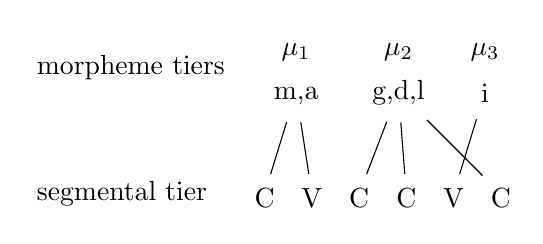
\begin{tikzpicture}[shorten >=2pt,shorten <=3pt, draw=black!100]
	\def \rowthreeht{4.4cm}
	\def \rowtwoht{3.8cm}
	\def \twopointfive{4.1cm}
	%\def \weightstwo{3.75cm}
	\def \rowoneht{2.5cm}
	%\def \weightsone{1.25cm}
	%\def \basement{2cm}
	\tikzstyle{c-node}=[text height=8pt,text centered,inner sep=3pt,minimum size=10pt]
	\tikzstyle{m-node}=[text height=7pt,text centered,inner sep=3pt,minimum size=12pt]
	\tikzstyle{r-node}=[text height=10pt,inner sep=0pt,minimum size=10pt]
	%\tikzstyle{d-node}=[text height=6pt,text centered,inner sep=0pt,minimum size=12pt]
	\tikzstyle{annot}=[text width=25ex,align=left]
	% labels
	\node[annot] (mtierstop) at (0cm,\twopointfive) {morpheme tiers};
	\node[annot] (segtier) at (0cm,\rowoneht) {segmental tier};
	%\node[annot] (mtiersbot) at (0cm,\basement) {};
	
	% surface layer
	\node[r-node] 	(r0)	at (1.0cm,\rowoneht)		{C};
	\node[r-node] 	(r1)	at (1.6cm,\rowoneht)		{V};
	\node[r-node] 	(r2)	at (2.2cm,\rowoneht)		{C};
	\node[r-node] 	(r3)	at (2.8cm,\rowoneht)	 	{C};
	\node[r-node] 	(r4)	at (3.4cm,\rowoneht)	 	{V};
	\node[r-node] 	(r5)	at (4.0cm,\rowoneht)	 	{C};
	
	% hidden-layer elements
	\node[r-node] 	(m0)	at (1.4cm,\rowthreeht)		{$\mu_{1}$};
	\node[r-node] 	(m1)	at (2.7cm,\rowthreeht)		{$\mu_{2}$};
	\node[r-node] 	(m2)	at (3.8cm,\rowthreeht)		{$\mu_{3}$};

	% hidden layer
	\node[c-node] 	(m3)	at (1.4cm,\rowtwoht)		{\/m,a\/};
	\node[c-node] 	(m4)	at (2.7cm,\rowtwoht)		{\/g,d,l\/};
	\node[c-node] 	(m5)	at (3.8cm,\rowtwoht)		{\/i\/};
		
	\path
		(m3)	edge	node	{}	(r0)
		(m3)	edge	node	{}	(r1)
		%
		(m4)	edge	node	{}	(r2)
		(m4)	edge	node	{}	(r3)
		(m4)	edge	node	{}	(r5)
		%
		(m5)	edge	node	{}	(r4);
		
	\end{tikzpicture}
	\label{subfig:nonlinear}
	}
%\caption{Autosegmental morphology} 
%Here we have a segmental tier, or CV skeleton, and three
%autosegmental morpheme tiers. Each morpheme tier is in fact a sequence of phonological feature bundles. We represent these these feature bundles as phonemes, i.e., characters m, a, g, d, i, and l.
%\textit{g.d.l} is in boldface.} % and the causative vocalization \textit{-i-}.}
%  interrupted by  The linear (single-tier) approach is unable to connect the \textit{r} to the \textit{zk}, while the multilinear approach is able to unite discontiguous elements through external morpheme ($\mu$) nodes.}
%\label{subfig:nonlinear}
%\vspace{-20pt}
%\vspace{1pt}
%\end{figure}

%\begin{wrapfigure}{R}{0.5\textwidth}
%\begin{figure}[htb]
%\centering
	\subfigure[Linear approach]{
	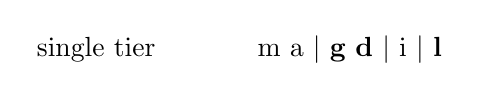
\begin{tikzpicture}[shorten >=1pt,draw=black!100]
	\vspace{50pt}
	\def \floor{0cm}
	\tikzstyle{f-node}=[text centered,inner sep=0pt] %text centered]
	\tikzstyle{annot}=[text width=34ex,align=left]
	% labels
	\node[annot] (floorlabel) at (0cm,\floor) {single tier};
	
	% surface layer
	\node[f-node] 	(f0)	at (1.4cm,\floor)			{m\,\,a\,\,$|$\,\,\textbf{g}\,\,\textbf{d}\,\,$|$\,\,i\,\,$|$\,\,\textbf{l}};
%	\node[f-node] 	(f1)	at (1.7cm,\floor)		{a};
%	\node[f-node] 	(f2)	at (2cm,\floor)		{$|$};
%	\node[f-node] 	(f3)	at (2.35cm,\floor)		{\textbf{g}};
%	\node[f-node] 	(f4)	at (2.65 cm,\floor)	 	{\textbf{d}};
%	\node[f-node] 	(f5)	at (3 cm,\floor)	 	{$|$};
%	\node[f-node] 	(f6)	at (3.3 cm,\floor)	 	{i};
%	\node[f-node] 	(f7)	at (3.6 cm,\floor)	 	{$|$};
%	\node[f-node] 	(f8)	at (3.9 cm,\floor)	 	{\textbf{l}};
	\end{tikzpicture}
\label{subfig:linear}
}
%\caption{Two approaches to analyzing \textit{hizkir} (`he reminded'), which has three morphemes. 
%The root \textit{z.k.r} (boldface) is discontinuous. The linear (single-tier) approach is unable to connect the \textit{r} to the \textit{zk}, while the multilinear approach is able to unite discontiguous elements through external morpheme ($\mu$) nodes.}
%%: an input layer ($\mathbf{d}$), a hidden layer ($\mathbf{m}$), and an output layer
\caption{Multiple tiers vs. a single tier}
\label{fig:linear}
%\vspace{-20pt}
%\vspace{1pt}
\end{figure}

Notice that $\mu_2$, the consonantal root, is discontinuous; it is
interrupted by $\mu_3$. If a model has only one tier, as in
fig.~\ref{subfig:linear}, there would be no way of representing the
unity of $\mu_2$, i.e., that \textit{g}, \textit{d}, and \textit{l}
all belong to the same morpheme. With this multi-tier aspect of
autosegmental morphology in mind, we can now state two criteria for a
model of non-concatenative morphology:
\begin{exe}
  \ex\begin{xlist} 
    \ex Morphemes are represented as being separate from the
    segmental tier.\label{ex:criterion1}
    \ex Each morpheme tier (or node) is orthogonal to all other
    morpheme tiers. \label{ex:criterion2}
\end{xlist}
\label{ex:criteria}
\end{exe}
%\begin{enumerate}
%\item We need more than one tier.
%\item Each tier must be orthogonal to every other tier. 
%\end{enumerate}
Criterion~(\ref{ex:criterion2}) implies that the morpheme tiers are
unordered.  Without sequential dependencies between
morpheme tiers, crossing edges such as those in
fig.~\ref{subfig:nonlinear} are made possible.
%The elements within a given tier must be independent; connections (or edges) are only valid if they are between elements of different tiers. 
%
%\marginpar{Think about the placement of this sentence}
%
We should note that autosegmental morphology has other properties to
constrain morphological structure, e.g., the well-formedness
principle; at present, we are not concerned with capturing all aspects
of autosegmental morphology, but instead in building a generic system
to which one can later add linguistically motivated constraints.

%Each tier is orthogonal to every other tier, which is to say that each tier is independent. This independence is crucial for capturing non-concatenative morphology. First, the collection of morpheme tiers needs to be separate, i.e., disjoint, from the segmental tier. Second, each morpheme tier needs to be orthogonal to (or independent of) every other morpheme tier. This is to say that morpheme tiers cannot be ordered with respect to other morpheme tiers. The \emph{components} of a morpheme tier can be ordered, but this internal ordering has no bearing on the components of other morpheme tiers. In \ref{fig:autosegmental}, for example, morphemes $\mu_2$ and $\mu_3$ each have arrays of components: /g,d,l/ and /i/, respectively. The components of $\mu_2$ are ordered relative to each other, but not relative to the /i/ of $\mu_3$
%a morpheme  is independent of the segmental tier comprising the phonological segments, it can associate with nonadjacent segments. 
%  The multi-linear architecture of autosegmental theory thus provides a means of
%dealing with nonconcatenative morphology \cite{mccarthy:1981}.


%and comprises one or more (not necessarily contiguous) feature bundles. Each feature bundle can associate with any phonological segment in the \emph{segmental tier} as long as the association lines of  
%Our objective here is to demonstrate how this
%multi-linear architecture can be implemented in a machine learning system so that it might learn
%% Explored in linguistic theory and computationally with hand-written grammars ...
%learn non-concatenative morphology (and do so without supervision).
%in a machine learning system capable of learning nonconcatenative morphology without supervision.
%During the course of development, I will explore different options for system components, e,g., the set of features,
%in order to arrive at the configuration that gives the best result for learning autosegmental morphology.  
\subsection{A graph-theoretic interpretation}

In graph-theoretic terms, the multi-linear formalism of
\cite{mccarthy:1981} is a type of \emph{multipartite}
%, or $K$-partite, 
graph. This is a graph whose nodes can be partitioned into $N$ sets of
\emph{mutually nonadjacent} nodes, i.e., $N$ sets such that no two
nodes within the \emph{same} set are connected by an edge. %---%
%In graph theory, an \emph{independent} set of nodes is one in which no two nodes are connected by an edge; i.e., it is a set of \emph{mutually nonadjacent} nodes.
% that is, $K$ sets which is to that a set of nodes, or partition, is defined by the \emph{lack} of connections between them. 
%while two nodes may be connected if each belongs to a different set.
%, but within the same set there are no
%connections. 
Fig.~\ref{fig:bipartite}, for example, shows a \emph{bipartite}
graph, i.e., a graph with two partitions, in this case the sets $M$
and $R$.
% i.e., a $K$-partite graph in which $K=2$. 
Within each set, all nodes are independent; the only connections are between nodes of different sets.

 \begin{figure}[htb]
 %\begin{minipage}{.3\textwidth}
 \begin{center}
 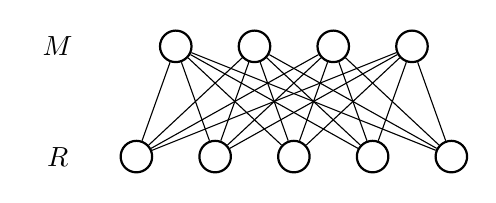
\begin{tikzpicture}[draw=black!100,scale=1.0]
 	\def \rowtwoht{1.4cm}
 	\def \rowoneht{0.0cm}
 	\tikzstyle{m-node}=[circle,draw=black!100,thick,inner sep=0pt,minimum size=4mm]
 	\tikzstyle{r-node}=[circle,draw=black!100,thick,inner sep=0pt,minimum size=4mm]
 	\tikzstyle{annot} = [text width=1.5em, text centered]
 	% labels
 	\node[annot] (hidden-label) at (-0.5cm,\rowtwoht) {$M$};
 	\node[annot] (surface-label) at (-0.5cm,\rowoneht) {$R$};
 %	\node[annot] (d-label) (0, 0) {observed data vector};
 	% hidden layer
 	\node[m-node] 	(m0)	at (1cm,\rowtwoht)		{};
 	\node[m-node] 	(m1)	at (2cm,\rowtwoht)		{};
 	\node[m-node] 	(m2)	at (3cm,\rowtwoht)	 	{};
 	\node[m-node] 	(m3)	at (4cm,\rowtwoht) 		{};
 	% surface layer
 	\node[r-node] 	(r0)	at (0.5cm,\rowoneht)		{};
 	\node[r-node] 	(r1)	at (1.5cm,\rowoneht)		{};
 	\node[r-node] 	(r2)	at (2.5cm,\rowoneht)	 	{};
 	\node[r-node] 	(r3)	at (3.5cm,\rowoneht) 		{};
 	\node[r-node] 	(r4) 	at (4.5cm,\rowoneht)   		{};
 	%\node[r-node] 	(r5) 	at (6.5cm,\rowoneht)   		{};
 	\path (r0)	edge	node	{}	(m0)
		(r0)	edge	node	{}	(m1)
		(r0)	edge	node	{}	(m2)
		(r0)	edge	node	{}	(m3)

		(r1)	edge	node	{}	(m0)
		(r1)	edge	node	{}	(m1)
		(r1)	edge	node	{}	(m2)
		(r1)	edge	node	{}	(m3)

		(r2)	edge	node	{}	(m0)
		(r2)	edge	node	{}	(m1)
		(r2)	edge	node	{}	(m2)
		(r2)	edge	node	{}	(m3)
						
		(r3)	edge	node	{}	(m0)
		(r3)	edge	node	{}	(m1)
		(r3)	edge	node	{}	(m2)
		(r3)	edge	node	{}	(m3)

		(r4)	edge	node	{}	(m0)
		(r4)	edge	node	{}	(m1)
		(r4)	edge	node	{}	(m2)
		(r4)	edge	node	{}	(m3);
 		%(m3)	edge	node	{}	(r5);		
 \end{tikzpicture}
 \end{center}
 \caption{Bipartite graph}
 %. Neither layer contains sequential dependencies; every unit is independent within its own layer. Each hidden unit is thus free to cause any combination of observed units.}
 \label{fig:bipartite}
 \end{figure}

% 
As it turns out, a bipartite graph suffices
%we do not need many partitions 
to capture the essential properties of McCarthy's autosegmental
framework,
% (fig.~\ref{subfig:nonlinear}). 
for a bipartite graph meets the two criteria stated in
(\ref{ex:criteria}).  We can reformulate the morpheme tiers and the
segmental tier in fig.~\ref{subfig:nonlinear} as the sets $M$ and
$R$, respectively, in fig.~\ref{fig:bipartite}---disjoint
by the definition of \emph{bipartite}. This satisfies the first
criterion. For the second, each node in $M$ represents a morpheme (or
morpheme tier), and, by the definition of \emph{bipartite}, the nodes
within $M$ are independent and thus orthogonal.

An MCMM (section~\ref{sec:mcmm}) is well-suited for the learning of
non-concatenative morphology because it is bipartite graph. It has two
\emph{layers} (equivalently, sets) of nodes, a hidden layer and a
surface layer---corresponding, respectively, to $M$ and $R$ in
fig.~\ref{fig:bipartite}. There are no intra-layer connections in an
MCMM, only connections between layers.
%, as in any bipartite graph.

We will henceforth refer to an MCMM's two partitions of nodes as
\emph{vectors} of nodes and will use matrix and vector notation to
describe the components of an MCMM:
%. That is, we will use
uppercase boldface letters refer to matrices, %(e.g., $\mathbf{M}$),
lowercase boldface letters refer to vectors,
% and matrix rows or columns, 
%(e.g., $\mathbf{m}_i$),
and italicized lowercase letters refer to the individual elements
of vectors/matrices. % (e.g., $m_{ik}$).
For example, $m_{i,k}$ is the $k^{\mathrm{th}}$ element in the vector
$\mathbf{m}_i$, which is the $i^{\mathrm{th}}$ row in the $I \times K$ matrix
$\mathbf{M}$. Thus, we will henceforth write the $M$ and $R$ in
fig.~\ref{fig:bipartite} as $\mathbf{m}$ and $\mathbf{r}$,
respectively (or $\mathbf{m}_i$ and $\mathbf{r}_i$, where $i$ is the
index of the $i^{\mathrm{th}}$ word).

%use matrix and vector notation to refer to an MCMM's components.
%That is, we will use lower-case bold-faced letters to refer an MCMM's two node partitions, since
%
%for each input datapoint $\mathbf{x}_i$, there is a vector of $K$ hidden nodes
%$\mathbf{m}_i$, and a vector of \emph{reconstruction} nodes $\mathbf{r}_i$.
%in which are independent and thus orthogonal by definition of \emph{bipartite}. and $R$ in fig.~\ref{subig:bipartite}, respectively. The morpheme  and the segmental tier as set $R$. If we think of $M$ as a multidimensional vector wherein each node (or element) constitutes a distinct dimension, then each node in $M$ is orthogonal to every other node. Each node in $M$, that is, acts as an autosegmental \emph{tier}. The segmental tier in fig.~\ref{subig:nonlinear} can be represented as the set $R$ in fig.~\ref{subig:nonlinear}.


% ***

% \marginpar{MD will start here: how can we quickly show that we're aware of the previous literature, without such a thorough exploration?}

% As \cite{mccarthy:1981} notes, strictly concatenative approaches to
% morphology acknowledge only the string as a level of representation.
% %segmental string.
% % (roughly, the string of phonemes). 
% Consequently, they must represent both the order of characters (or
% phonemes) and their morphological grouping within the same linear
% string.
% % The problem is that morphemes are not always contiguous, and
% % %as we saw above in the case of Hebrew, and 
% % %Many languages exhibit non-concatenative processes, and in such cases. 
% % a linear analysis has no straightforward means of treating a discontinuous subsequence as a unified morpheme.
% %, i.e., as a single unit with a single, unified set of properties.
% %, i.e., a truly unified morpheme. 
% McCarthy offers a nonlinear formalism with morphemes represented as
% nodes on autosegmental tiers, allowing
% %, i.e., tiers that are separate from the segmental string. 
% %Separating tiers from the segmental string allows 
% %morpheme-phoneme 
% associations between morphemes and segments to be independent of the
% order \citep[cf., e.g.,][]{kiraz:96}.
% %segments' linear arrangement.
% %
% % This formulation turns out to be highly general, for it treats
% % concatenative and non-concatenative processes with the same formal
% % machinery.
% %
% %as fundamentally different; it uses the same formal machinery whether morphemes are continuous or discontinuous.
% % Carry over framework to unsupervised morpheme segmentation?
% %
% Following McCarthy, we 
% % distinguish ``linear vs. nonlinear" conceptual framework to categorize existing approaches in the field of unsupervised morpheme segmentation.
% % In the following discussion, 
% use \textbf{nonlinear} to refer to algorithms employing one or more
% \textit{hidden layers} to encode the structure of the \textit{surface
%   layer}.
% %, the layer of the graphemes/phonemes.
% % Here, \textit{hidden layer} is conceptually related to McCarthy's
% % \textit{autosegmental tier}, but the two terms are not necessarily
% % equivalent formally.  
% We use \textbf{linear} (cf. `one-dimensional') to refer to algorithms
% referencing only the surface layer 
% %of graphemes 
% in the representation of morphology.
% %ical structure.
% % , e.g., by annotating the
% % surface string itself with morpheme boundary symbols.
% % This definition is not unlike ``one dimensional," a fairly common
% % sense of \textit{linear}.  We do not, however, use \textit{linear} to
% % mean ``in/like a straight line."
% %but one to be distinguished from ``in/like a straight line." As it is used in this paper, the term \textit{linear} s not related in any direct way to the notions of line and straightness.
% %We do not, however, use \textit{linear} to mean ``in a straight line" or even ``like a straight line."
% %
% We divide 
% %each of 
% these into
% %\textit{linear} and \textit{nonlinear} each into a 
% \textbf{sequential} and \textbf{non-sequential} subcategories.

%, obtaining four categories in all. We describe each below.
%
% Note that a \textit{morphological classification decision} can simply
% be a binary split decision, i.e., a decision between the classes
% ``part of the current morpheme" and ``part of the next morpheme."
%\begin{itemize}
%\item Given a sequence of morpheme classification decisions, each decision depends on the preceding chain of decisions.
%\item Given a sequence of candidate morpheme split points, each split decision depends on the preceding chain of split decisions. either the preceding representational units or succeither immediately left or immediately right), where \textit{representational unit} is a grapheme if the algorithm is linear and a hidden variable if the algorithm is nonlinear. 
% A \textit{morpheme segmentation decision} is, broadly speaking, an answer to the question, ``What is the morphological category/status of the current representational unit? (e.g., Does the current unit begin a new segment?)"
%\item The dependencies in the sequence all go in the same direction.
%\end{itemize}
% This gives us a total of four categories: sequential linear (SL),
% non-sequential linear (NSL), sequential non-linear (SNL), and finally
% non-sequential nonlinear (NSNL). 

%We will now discuss and exemplify each of these categories in turn.

% \paragraph{Sequential linear algorithms}
% \label{subsec:seq-lin}

% \marginpar{SK: ``decision'' = sequential information or sequential
%   processing? (MD: information, I think?  not entirely sure) ... how
%   about ``each segmentation decision is dependent upon a previous
%   one''}

%``I have the suspicion that you are switching between sequential processing and sequential information, on which the decisions are based. They do not necessarily coincide. You can have an algorithm that performs non-sequential processing while using sequential information, or the other way round. Your definition on p. 4 is based on "decisions", which I read as processing.''}

% In a \textbf{sequential linear (SL)} algorithm, 
% %represented in fig.~\ref{fig:seq-lin}, 
% each segmentation decision depends on an immediately preceding
% context, and there are no non-surface-layer representational units.
% % The first unsupervised morpheme segmentation algorithms were sequential linear algorithms.
% The earliest example is the Letter Successor Variety (LSV) method
% \citep{harris:1955, harris:1967}; different techniques are covered in
% \citet{hammarstrom:2011}.
% % Given a corpus
% % %  $W$
% % and a string $x$, $\mathrm{LSV}(x)$ is the number of letter
% % \textit{types}
% % %(as opposed to \textit{tokens}) 
% % that occur in the next position following $x$ whenever $x$ is an
% % initial substring of a word.
% % $w$ in $W$.
% % Letter Predecessor Variety (LPV) is the same measure, except the substring $x$ is word-final rather than word-initial, and the direction of the algorithm is reversed. 
% % $\mathrm{LSV}(x)$ is used to find prefix-stem boundaries, while $\mathrm{LPV}(x)$ is used to find stem-suffix boundaries.
% %
% % Stress sequential nature of algorithm
% % The different techniques for using LSV to discover morpheme boundaries
% % %, such as the ``peak and plateau'' technique
% % \citep[see][]{hammarstrom:2011} rely on the intuition that at any
% % given point within a morpheme, the next letter is fairly predictable,
% % i.e., has a smaller number of succeeding letter types.
% % But at the border between two morphemes, the
% % next letter is much less predictable.
% More recent linear sequential methods
% %have thus abandoned LSV/LPV, often in favor of
% use frequency-based heuristics, such as pointwise mutual information
% \citep{goldsmith:2001} or trie-based affix-finding
% \citep{moon-et-al:2009} to predict morpheme boundaries.
% % , for example, uses a score based on pointwise mutual information
% % (PMI) to approximate the likelihood that a given character $n$-gram
% % %$c_{1}c_{2}...c_{n}$ 
% % is a morphemic unit.
% % In particular, the PMI of the characters $c_{1},
% % c_{2}, ..., c_{n}$ is multiplied by the relative frequency of the
% % $n$-gram $c_{1}c_{2}...c_{n}$. \cite{goldsmith:2001} obtains candidate
% % suffixes by taking the $n$-grams that are ranked highest according to
% % this score.
% %(i.e., the count of $c_{1}c_{2}...c_{n}$ divided by the total count of all $n$-grams).  
% %
% %Moon
% % \cite{moon-et-al:2009} apply tries to the task of finding stems and
% % affixes, to store recurring character sequences.
% %, as have a number of other researchers. 
% % Tries are useful for learning concatenative morphology because they
% % compactly store recurring character sequences.
% %that are repeated a group of words. by sets of words beginning with the same character. 
% % Each node in a trie represents a certain prefix string (with the root node representing the empty string), 
% % and every path proceeding out from a node represents a possible succeeding character. 
% % Thus, even though tries are tree data structures, 
% In all cases, the methods process data in a sequential manner and
% lack hidden nodes for morphological relationships.
% % linearly, lacking hidden nodes.

% ; one of them is the ``peak and plateau" technique, which works as follows:
% \begin{itemize}
% \item Given an $n$-length word $w$ whose graphemes are indexed from 0 to $n$, compute $\mathrm{LSV}(w[0:i])$ for each $i$ in the range $[0, n)$. \item Insert a morpheme boundary after the substring $w[0:i]$ if and only if $\mathrm{LSV}(w[0:i-1]) \le \mathrm{LSV}(w[0:i]) \ge \mathrm{LSV}(w[0:i+1])$, i.e., there is a local peak in the LSV sequence at index $i$.
% \end{itemize}
% Notice the sequential nature of this technique: each LSV calculation is determined solely by the immediately preceding string of graphemes. Note also its linearity: there is only a single layer of representation for both the grapheme sequence and the morphological analysis.

% \begin{figure}[tb]
% %\begin{minipage}{.3\textwidth}
% \begin{center}
% \begin{tikzpicture}[shorten >=1pt,->,draw=black!100,node distance = 1.3cm, auto]]
% 	\def \startnode{1.5cm}
% %	\def\secondrow{1.0cm}
% 	\tikzstyle{r-node}=[circle,draw=black!100,thick,inner sep=0pt,minimum size=4mm]
% 	\tikzstyle{annot} = [text width=2.5cm, text centered]
% %	\tikzstyle{annot} = [text width=2.0cm, text centered]
% 	% labels
% %	\node[annot] (m-label) at (0,\thirdrow) {hidden-unit vector};
% %	\node[annot] (r-label) at (0, \secondrow) {prediction vector};
% %	\node[annot] (d-label) (0, 0) {observed data vector};
% 	% hidden layer
% 	\node[annot] (surface-label) at (0cm,0cm) {surface layer};
% %	\node[annot] (r-label) at (0, \secondrow) {prediction vector};
% %	\node[annot] (d-label) (0, 0) {observed data vector};
	
% 	% surface layer
% 	\node[r-node] 	(r0)	at (\startnode,0cm)		{};
% 	\node[r-node] 	(r1)	at (2.5cm, 0cm)		{};
% 	\node[r-node] 	(r2)	at (3.5cm,0cm)	 	{};
% 	\node[r-node] 	(r3)	at (4.5cm,0cm) 		{};
% 	\node[r-node] 	(r4) 	at (5.5cm,0cm)   		{};
	
% 	\path (r0)	edge	node	{}	(r1)
% 		(r1)	edge	node	{}	(r2)
% 		(r2)	edge	node	{}	(r3)
% 		(r3)	edge	node	{}	(r4);
% \end{tikzpicture}
% \end{center}
% \caption{Sequential linear architecture}
% %. Each representational unit depends on the preceding unit, and no unit exists outside of the surface layer.}
% \label{fig:seq-lin}
% \end{figure}

% The intuition behind the LSV/LPV method is related to that behind the entropy-based methods in natural language processing:
% %In fact, LSV generally increases/decreases as entropy increases/deceases: 
% At any given point \emph{within} a morpheme, the next letter is fairly predictable, which generally coincides with a smaller number of succeeding letter types. But at the border between two morphemes, the next letter is much less predictable. This low predictability generally translates to a much larger set of options for the succeeding letter (i.e., a higher LSV). However, it out that LSV is not always a reliable indicator of morpheme boundaries. \cite{hammarstrom:2011}, for example, provide LPV counts for the word \textit{disturbance}. 
% The highest count (25) 
% %(i.e., 25 of the 26 possible letters in the English alphabet) 
% occurs between \textit{disturbanc} and \textit{e}, An LPV-based analysis would thus yield an incorrect result in this case, a consequence of the fact that \textit{e} is such a ubiquitous word-final letter in English spelling. 

%Goldsmith
% More recent linear sequential methods
% %have thus abandoned LSV/LPV, often in favor of
% use frequency-based heuristics.  \cite{goldsmith:2001}, for example,
% uses a score based on pointwise mutual information (PMI) to
% approximate the likelihood that a given character $n$-gram
% %$c_{1}c_{2}...c_{n}$ 
% is a morphemic unit.
% % In particular, the PMI of the characters $c_{1},
% % c_{2}, ..., c_{n}$ is multiplied by the relative frequency of the
% % $n$-gram $c_{1}c_{2}...c_{n}$. \cite{goldsmith:2001} obtains candidate
% % suffixes by taking the $n$-grams that are ranked highest according to
% % this score.
% %(i.e., the count of $c_{1}c_{2}...c_{n}$ divided by the total count of all $n$-grams).  
% %
% %Moon
% \cite{moon-et-al:2009} apply tries to the task of finding stems and
% affixes, to store recurring character sequences.
% %, as have a number of other researchers. 
% % Tries are useful for learning concatenative morphology because they
% % compactly store recurring character sequences.
% %that are repeated a group of words. by sets of words beginning with the same character. 
% % Each node in a trie represents a certain prefix string (with the root node representing the empty string), 
% % and every path proceeding out from a node represents a possible succeeding character. 
% % Thus, even though tries are tree data structures, 
% In all cases, the methods process data in a sequential manner and
% represent morphological relationships linearly, lacking hidden nodes.

% , and every path through a trie is deterministic.
% \cite{moon-et-al:2009} depart from other trie-based methods in using
% document boundaries to approximate semantic context.  This helps them
% weed out spurious analyses like the \textit{disturbanc}+\textit{e}
% example above, but it does not change the fundamentally sequential and
% linear nature of their approach.

% \paragraph{Non-sequential linear algorithms}
% \label{subsec:nonseq-lin}

% In a \textbf{non-sequential linear (NSL)} algorithm, 
% %illustrated in fig.~\ref{fig:nonseq-lin}, 
% there are no dependencies between representational units, but also no
% hidden units.
% %; i.e., all representational units reside in the surface layer.  
% As one example, \cite{poon-et-al:2009} use log-linear models to induce
% morphological segmentations for Arabic and Hebrew. 
% % Their algorithm
% % searches for the set of parameters $\theta$ that maximizes the joint
% % probability of a corpus $W$ and a segmentation $S$ (i.e., $P(W,S|
% % \theta)$).
% % = P(W|S; \theta) \cdot P(S| \theta)$.
% %They generate candidate segmentations via Gibbs sampling. For each candidate, they extract a feature set
% % Log-linear models are well-suited for large numbers of arbitrarily
% % defined features.
% % \cite{poon-et-al:2009} use morpheme features and morpheme context
% % features.  The former category specifies a morpheme type and its
% % frequency, e.g., \texttt{vlav:1} and \texttt{w:2}.  The latter
% % category indicates the character bigrams to the left and right of a
% % given morpheme, e.g., \texttt{\#w\_wn:1} (a word boundary followed by
% % the character \textit{w} on the left and the characters \textit{w} and
% % \textit{n} on the right).  Note, however, that one could use any type
% % of feature or combination of feature types with a log-linear
% % model. One could, for example, have features representing both
% % continuous and discontinues bigrams in the same feature set.
% %
% %However, one in principle could use any sort of feature in a log linear model, such as a feature type representing discontinuous bigrams, for example.
% %Each feature represents the both corpus and the segmentation jointly, and a fully specified set of features thus represents an entire segmented corpus;
% %but there is no limit on the variety or quantity of features one can incorporate into a log-linear model.
% % Why is a log linear model non-sequential?
% Log-linear models are non-sequential because they treat all features
% as independent, estimating a global joint probability.
% %for the entire bag of features.
% % Sequential models, in contrast, estimate conditional probabilities
% % based on sequential dependencies between features.
% % Why is Poon et al's algorithm linear?
% % \cite{poon-et-al:2009} incorporate no latent variables,
% % %, however, 
% % %Their representation of morphological structure makes 
% % referencing only the the surface layer of graphemes.
% % Their morpheme
% % features are limited to continuous grapheme sequences, and their
% % morpheme context features encode only extreme left and right contexts,
% % thus assuming no internal boundaries (i.e., no morpheme
% % interruptions).  
% Even though such a model allows for any type of feature, including
% both continuous and discontinuous $n$-grams,
% %They generate candidate segmentations via Gibbs sampling, but, for an $n$-length word, they consider  
% the algorithm ultimately can only isolate stems and affixes, because
% it only acknowledges the surface layer of text.
% %, and not discontinuous roots and patterns.
% % of Arabic and Hebrew.

% \begin{figure}[tb]
% %\begin{minipage}{.3\textwidth}
% \begin{center}
% \begin{tikzpicture}[shorten >=1pt,->,draw=black!100]
% 	\def \startnode{1.5cm}
% %	\def\secondrow{1.0cm}
% 	\tikzstyle{r-node}=[circle,draw=black!100,thick,inner sep=0pt,minimum size=4mm]
% 	\tikzstyle{annot} = [text width=2.5cm, text centered]
% 	% labels
% 	\node[annot] (surface-label) at (0cm,0cm) {surface layer};
% %	\node[annot] (r-label) at (0, \secondrow) {prediction vector};
% %	\node[annot] (d-label) (0, 0) {observed data vector};
	
% 	% surface layer
% 	\node[r-node] 	(r0)	at (\startnode,0cm)		{};
% 	\node[r-node] 	(r1)	at (2.5cm, 0cm)		{};
% 	\node[r-node] 	(r2)	at (3.5cm,0cm)	 	{};
% 	\node[r-node] 	(r3)	at (4.5cm,0cm) 		{};
% 	\node[r-node] 	(r4) 	at (5.5cm,0cm)   		{};
	
% %	\path (r0)	edge	node	{}	(r1)
% %		(r1)	edge	node	{}	(r2)
% %		(r2)	edge	node	{}	(r3)
% %		(r3)	edge	node	{}	(r4);
% \end{tikzpicture}
% \end{center}
% \caption{Non-sequential linear architecture}
% %. No dependencies exist between representational units, and no unit exists outside of the surface layer.}
% \label{fig:nonseq-lin}
% \end{figure}

% \cite{poon-et-al:2009} use morpheme features and morpheme context
% features.  The former category specifies a morpheme type and its
% frequency, e.g., \texttt{vlav:1} and \texttt{w:2}.  The latter
% category indicates the character bigrams to the left and right of a
% given morpheme, e.g., \texttt{\#w\_wn:1} (a word boundary followed by
% the character \textit{w} on the left and the characters \textit{w} and
% \textit{n} on the right).  Note, however, that one could use any type
% of feature or combination of feature types with a log-linear
% model. One could, for example, have features representing both
% continuous and discontinues bigrams in the same feature set.


% \paragraph{Sequential nonlinear algorithms}
% \label{subsec:seq-nonlin}
% I need to say what the nonlinear aspect brings to the table. If being nonlinear is beneficial, sequential nonlinear algorithms should be better than sequential linear ones. So what do sequential nonlinear algorithms have that sequential linear algorithms don't? How does being nonlinear help them?
% First, what sort of algorithms are sequential nonlinear?

% \textbf{Sequential nonlinear (SNL)} algorithms
% %, illustrated in fig.~\ref{fig:seq-nonlin}, 
% differ from sequential
% linear ones by adding a layer of hidden units for encoding the
% structure of the surface layer.
% %This makes them nonlinear. 
% % They are still sequential, however, in that there are sequential
% % dependencies within the hidden layer.
% %; i.e., each hidden unit depends on its predecessor hidden unit(s).
% The prototypical example of a sequential nonlinear model is the Hidden
% Markov Model (HMM).  \cite{creutz-and-lagus:2005,
%   creutz-and-lagus:2007} employ an HMM to induce a morphological
% lexicon.
% %, i.e., a list of morpheme-like segments.
% %that they call \textit{morphs}.
% %sorted in order of increasing morph length. 
% %They take a maximum a posteriori (MAP) approach.
% The hidden layer in this case serves to facilitate the search for the optimal lexicon 
% (i.e., segmentation) by providing a means of abstracting away from the literal segments themselves.

% % Their algorithm seeks to find the lexicon such that $P(lexicon|corpus)$ is maximized, which, due to Bayes' theorem, equates to finding the lexicon that maximizes $P(corpus|lexicon) \cdot P(lexicon)$. The probability $P(corpus|lexicon)$ is computed by a first-order HMM with five hidden states representing the positional morpheme types \textsc{prefix}, \textsc{stem}, \textsc{suffix}, \textsc{non} (for non-morpheme), and a special word-boundary category. The observation sequence is a segmentation hypothesis, i.e., a candidate segmentation of the corpus into morphs. Candidate segmentations are generated independently of the HMM, as are the transition and emission probabilities. The HMM's only unknown is thus the most likely hidden state sequence, which is computed by the Viterbi algorithm, along with the probability $P(corpus|lexicon)$.
% % The hidden layer in this case serves only to facilitate the search for the optimal lexicon 
% % (i.e., segmentation) by providing a means of abstracting away from the literal segments themselves.
% %leaving the sequence of hidden states as the HMM's only unknown.
% %The HMM's role is to evaluate each candidate morph sequence. 

% took out the "h"
% \begin{figure}[tb]
% %\begin{minipage}{.3\textwidth}
% \begin{center}
% \begin{tikzpicture}[shorten >=1pt,->,draw=black!100]
% 	\def \rowtwoht{1.0cm}
% 	\def \rowoneht{0.0cm}
% 	\tikzstyle{m-node}=[circle,draw=black!100,thick,inner sep=0pt,minimum size=4mm]
% 	\tikzstyle{r-node}=[circle,draw=black!100,thick,inner sep=0pt,minimum size=4mm]
% 	\tikzstyle{annot} = [text width=2.5cm, text centered]
% 	% labels
% 	\node[annot] (hidden-label) at (0cm,\rowtwoht) {hidden layer};
% 	\node[annot] (surface-label) at (0cm,\rowoneht) {surface layer};

% %	\node[annot] (d-label) (0, 0) {observed data vector};
	
% 	% hidden layer
% 	\node[m-node] 	(m0)	at (1.5cm,\rowtwoht)		{};
% 	\node[m-node] 	(m1)	at (2.5cm,\rowtwoht)		{};
% 	\node[m-node] 	(m2)	at (3.5cm,\rowtwoht)	 	{};
% 	\node[m-node] 	(m3)	at (4.5cm,\rowtwoht) 		{};
% 	\node[m-node] 	(m4) 	at (5.5cm,\rowtwoht)   		{};
	
% 	% surface layer
% 	\node[r-node] 	(r0)	at (1.5cm,\rowoneht)		{};
% 	\node[r-node] 	(r1)	at (2.5cm,\rowoneht)		{};
% 	\node[r-node] 	(r2)	at (3.5cm,\rowoneht)	 	{};
% 	\node[r-node] 	(r3)	at (4.5cm,\rowoneht) 		{};
% 	\node[r-node] 	(r4) 	at (5.5cm,\rowoneht)   		{};
	
% 	\path (m0)	edge	node	{}	(m1)
% 		(m1)	edge	node	{}	(m2)
% 		(m2)	edge	node	{}	(m3)
% 		(m3)	edge	node	{}	(m4);
		
% 	\path (m0)	edge	node	{}	(r0)
% 		(m1)	edge	node	{}	(r1)
% 		(m2)	edge	node	{}	(r2)
% 		(m3)	edge	node	{}	(r3)
% 		(m4)	edge	node	{}	(r4);
			
% \end{tikzpicture}
% \end{center}
% \caption{Sequential nonlinear architecture}
% % . Sequential dependencies only exist between hidden units, 
% % not between the observed units of the surface layer. The hidden units ``cause" the surface units.}
% \label{fig:seq-nonlin}
% \end{figure}

% \paragraph{Non-sequential nonlinear algorithms}
% \label{subsec:nonseq-nonlin}
% % Intro

% % Both sequential nonlinear (SNL) algorithms and \textit{non}-sequential
% % nonlinear (NSNL) algorithms posit hidden units that cause the observed
% % units of the surface layer.  
% In \textbf{non-sequential nonlinear (NSNL)} algorithms, neither the
% surface layer nor any hidden layers contain sequential dependencies.
% %, as shown in fig.~\ref{fig:nonseq-nonlin}.
% % Thus, every node---whether hidden or surface---is entirely independent
% % within its own layer.
% This intra-layer independence allows a hidden unit to associate with
% any combination of surface units.
% %, whether continuous or discontinuous
% %(see Figure \ref{fig:nonseq-nonlin}).
% %
% % \begin{figure}[tb]
% % %\begin{minipage}{.3\textwidth}
% % \begin{center}
% % \begin{tikzpicture}[shorten >=1pt,->,draw=black!100,scale=.95]
% % 	\def \rowtwoht{1.25cm}
% % 	\def \rowoneht{0.0cm}
% % 	\tikzstyle{m-node}=[circle,draw=black!100,thick,inner sep=0pt,minimum size=4mm]
% % 	\tikzstyle{r-node}=[circle,draw=black!100,thick,inner sep=0pt,minimum size=4mm]
% % 	\tikzstyle{annot} = [text width=2.5cm, text centered]
% % 	% labels
% % 	\node[annot] (hidden-label) at (0cm,\rowtwoht) {hidden layer};
% % 	\node[annot] (surface-label) at (0cm,\rowoneht) {surface layer};
% % %	\node[annot] (d-label) (0, 0) {observed data vector};
% % 	% hidden layer
% % 	\node[m-node] 	(m0)	at (2.5cm,\rowtwoht)		{};
% % 	\node[m-node] 	(m1)	at (3.5cm,\rowtwoht)		{};
% % 	\node[m-node] 	(m2)	at (4.5cm,\rowtwoht)	 	{};
% % 	\node[m-node] 	(m3)	at (5.5cm,\rowtwoht) 		{};
% % 	% surface layer
% % 	\node[r-node] 	(r0)	at (1.5cm,\rowoneht)		{};
% % 	\node[r-node] 	(r1)	at (2.5cm,\rowoneht)		{};
% % 	\node[r-node] 	(r2)	at (3.5cm,\rowoneht)	 	{};
% % 	\node[r-node] 	(r3)	at (4.5cm,\rowoneht) 		{};
% % 	\node[r-node] 	(r4) 	at (5.5cm,\rowoneht)   		{};
% % 	\node[r-node] 	(r5) 	at (6.5cm,\rowoneht)   		{};
% % 	\path (m0)	edge	node	{}	(r0)
% % 		(m1)	edge	node	{}	(r1)
% % 		(m2)	edge	node	{}	(r3)
% % 		(m1)	edge	node	{}	(r2)
% % 		(m1)	edge	node	{}	(r4)
% % 		(m3)	edge	node	{}	(r5);		
% % \end{tikzpicture}
% % \end{center}
% % \caption{Non-sequential nonlinear architecture}
% % %. Neither layer contains sequential dependencies; every unit is independent within its own layer. Each hidden unit is thus free to cause any combination of observed units.}
% % \label{fig:nonseq-nonlin}
% % \end{figure}
% %
% The NSNL category can take many forms.  \cite{baroni-et-al:2002}, for
% example, implicitly detect hidden units by computing edit distance for
% pairs of words.
% % The
% % Levenshtein algorithm finds the minimum number of edit operations
% % (typically allowing substitutions, deletions, and insertions) required
% % to change a \textit{source} word into a \textit{target} word.  In
% % addition to edit distance and edit operations, the algorithm can align
% % the characters of the source with those of the target word.  
% % From an alignment, one can extract the two words' 
% % %(potentially discontinuous) 
% % common subsequence.  
% % Thus, one may view the alignment as showing
% % %indicative of
% % a single hidden unit behind the surface occurrences of the
% % subsequence.
% % For example, for the Hebrew words \textit{dibr} `he spoke' and
% % \textit{mdbr} `he is speaking', the discontinuous root \textit{d.b.r }
% % is found.
% % Of course, a common subsequence does not necessarily indicate a
% % morphological relationship; consider, for instance, the English pair
% % To avoid finding spurious relationships
% % (cf. \textit{pork}/\textit{park}), \cite{baroni-et-al:2002} compute a
% % semantic similarity score, based on mutual information, to combine
% % with this orthographic similarity.
% % based on minimum edit distance.
% %orthographic similarity score.
% %
% \citet{rodrigues-and-cavar:2005} and
% \citet{goldsmith-and-xanthos:2009}, among others, simulate a
% multi-tier representation by separating learning into phases.
% %\citep[e.g.,][]{rodrigues-and-cavar:2005, goldsmith-and-xanthos:2009}.
% The first phase classifies individual characters into abstract,
% potentially discontinuous categories that subsequent concatenative
% phases use for finer-grained analysis.
% %
% \citet{botha:blunsom:13} explicitly define hidden layers via a grammar
% formalism which can capture discontiguous units.  As the grammars are
% mildly context-sensitive, the algorithm has a large complexity for
% morphological parsing, but in practice is effective.
% %
% % Other authors simulate a multi-tier representation by separating the
% % learning process into phases \citep[e.g.,][]{rodrigues-and-cavar:2005,
% %   goldsmith-and-xanthos:2009}: the first phase classifies individual
% % characters into abstract, potentially discontiguous categories that
% % subsequent concatenative phases can use for finer-grained analysis.
% %
% %\citet{botha:blunsom:13} explicitly define hidden layers via a grammar
% %formalism which can capture discontiguous units.  As the grammars are
% %mildly context-sensitive, the algorithm has a large complexity for
% %morphological parsing, but in practice is effective.
% %
% Both \citet{rodrigues-and-cavar:2005} and
% \citet{botha:blunsom:13} constrain the search for discontinuous roots
% by requiring triliteral roots (though quadrilateral roots exist) and
% encoding grammatical knowledge.  We explore a more general algorithm.


% While these approaches can detect discontinuous morphemes, they are
% limited, for example,
% % using an arbitrary threshold of 0.5 for two words to be similar enough
% % to share a root.
% % Baroni
% %% Mucho filtering
% % The algorithm of \cite{baroni-et-al:2002} must filter out a large
% % proportion of its input corpus, accepting only the words with relative
% % frequencies of less than 0.01 percent, presumed to be content words.
% % %% Arbitrary thresholds
% % It also relies on arbitrary thresholds; e.g., the threshold for
% % orthographic similarity measure (i.e., $1 - $ normalized minimum edit
% % distance) is set at 0.5, although their is no obvious reason why this
% % should be so.  Note also that behind this threshold is the assumption
% % that morphologically related words share at least half of their
% % characters, which is not necessarily true. It would be especially
% % problematic for agglutinative languages, in which relatively short
% % stems are frequently combined with long strings of affixes.  
% the edit distance approach only
% %\citep{baroni-et-al:2002} only 
% %being capable of 
% expressing pairwise relationships.
% % comparing words pairwise, and thus morphological
% % relationships can only be expressed on a pairwise basis. 
% % This limitation can be regarded as a consequence of the lack of an
% % explicitly-encoded hidden causal layer; 
% By contrast, an explicit hidden layer could mediate multi-way
% relationships in the surface layer.
% Rodrigues and Cavar
%% Only tri-literal roots
% \cite{rodrigues-and-cavar:2005} 
% %(following \cite{elghamry:2005})
% reduce the complexity of the search for discontinuous roots by
% requiring triliteral roots.  However, quadriliteral roots are not
% uncommon in Hebrew or Arabic, and
% %% Reasonable constraints, but constraints nonetheless. A truly general algorithm wouldn't need constraints. 
% % The two constraints on candidate-root generation are otherwise quite reasonable, but they are particular to the case of Semitic morphology. 
% a truly general algorithm would not require such constraints.  
% % In general, none of these works represent both the hidden layer and
% % surface layer simultaneously in a single model. In contrast, 
% % The NSNL model we use explicitly represents both surface and hidden
% % nodes in a single graphical model.

% \begin{figure}[htb!]
% %\begin{minipage}{.3\textwidth}
% \begin{center}
% \begin{tikzpicture}[draw=black!100]
% 	%[shorten >=1pt,->,draw=black!100]
% 	\def \rowtwoht{1.5cm}
% 	\def \rowoneht{0.0cm}
% 	\tikzstyle{m-node}=[circle,draw=black!100,thick,inner sep=0pt,minimum size=6mm]
% 	\tikzstyle{r-node}=[circle,draw=black!100,thick,inner sep=0pt,minimum size=6mm]
% 	\tikzstyle{annot} = [text width=2.5cm, text centered]
% 	% labels
% 	\node[annot] (hidden-label) at (0cm,\rowtwoht) {target};
% 	\node[annot] (surface-label) at (0cm,\rowoneht) {source};

% %	\node[annot] (d-label) (0, 0) {observed data vector};
	
% 	% hidden layer
% 	\node[m-node] 	(m0)	at (2.5cm,\rowtwoht)		{m};
% 	\node[m-node] 	(m1)	at (3.5cm,\rowtwoht)		{d};
% 	\node[m-node] 	(m2)	at (4.5cm,\rowtwoht)	 	{b};
% 	\node[m-node] 	(m3)	at (5.5cm,\rowtwoht) 		{r};
	
% 	% surface layer
% 	\node[r-node] 	(r0)	at (2.5cm,\rowoneht)		{d};
% 	\node[r-node] 	(r1)	at (3.5cm,\rowoneht)		{i};
% 	\node[r-node] 	(r2)	at (4.5cm,\rowoneht)	 	{b};
% 	\node[r-node] 	(r3)	at (5.5cm,\rowoneht) 		{r};
% 	%\node[r-node] 	(r4) 	at (6.5cm,\rowoneht)   		{};
% 	%\node[r-node] 	(r5) 	at (7.5cm,\rowoneht)   		{};
	
% 	\path (m1)	edge	node	{}	(r0)
% 		(m2)	edge	node	{}	(r2)
% 		(m3)	edge	node	{}	(r3);
% %		(m3)	edge	node	{}	(r3)
% %		(m1)	edge	node	{}	(r4)
% %		(m3)	edge	node	{}	(r5);
		
% \end{tikzpicture}
% \end{center}
% \caption{The minimum-edit-distance alignment for the Hebrew words \textit{dibr} `he spoke' and \textit{mdbr} `he is speaking'. The discontinuous root \textit{d.b.r } is discovered by aligning \textit{dibr} with \textit{mdbr} and extracting the common subsequence.}
% \label{fig:lev-align}
% \end{figure}
%The alignment implies a single cause behind both occurrences of the subsequence \textit{dbr}.
% Rest
 
% Other authors simulate a multi-tier representation by separating the
% learning process into phases.  The first phase classifies individual
% characters into abstract categories that subsequent phases use for
% finer-grained analysis.
% % Multiple phases
% % % that are temporally separate can
% % thus replicate what is achieved by multiple simultaneous levels of
% % representation.
% This is the approach that \cite{rodrigues-and-cavar:2005} take to
% induce the non-concatenative morphology of Arabic.
% %Following the statistical constraint-based method of \cite{elghamry:2005}, 
% Their first phase identifies root radicals \citep{elghamry:2005} and
% selects a root.
% % following the statistical constraint-based method of
% % \cite{elghamry:2005}.
% % For each word in their corpus, they generate a set of candidate
% % triliteral roots according to constraints derived from the tendencies
% % of Arabic roots as observed in corpora.  In particular, any 3-length
% % subsequence is admitted into the candidate set if and only if it
% % satisfies both of the following:
% % %, which in Arabic comprise both a consonantal root and a vocalic pattern. A string is allowed into a word's candidate stem set if and only if it satisfies the following constraints, which are based on the tendencies of Arabic roots as observed in corpora. 
% % (1) No two consecutive radicals may be separated by more than two characters, and (2) ``the distance between the first and third radicals cannot be greater than five" \citep[][p. 3]{elghamry:2005}. 
% % Then, a statistical score is computed for each candidate, and the one
% % with the highest score is selected as the root.  Once the roots 
% % %(and thus the stems) 
% % have been determined,
% %by the first phase, the second phase 
% Then, concatenative affixes are isolated through a separate
% methodology.
% %
% % Goldsmith and Xanthos
% An alternative first-phase strategy can be found in
% \cite{goldsmith-and-xanthos:2009}, who induce
% % present methods for partitioning a phonemic inventory into a class of
% % consonants and a class of vowels, thereby creating a CV template
% a CV template similar to the segmental tier of autosegmental
% phonology.

% An algorithm could use these classes to label each
% phoneme/grapheme in a string as either a consonant or vowel, thus
% creating a sort of CV skeleton or template similar to the segmental
% tier of autosegmental phonology.  Such a template would be helpful to
% subsequent phases as they go about isolating the root, pattern, and
% other morphemes.
%To delimit distinct morphemes, the linear approach must 

% Multiple Cause Mixture Model (MCMM) \citep{saund:93, saund:94} is an
% NSNL algorithm that explicitly represents both surface and hidden
% nodes in a single graphical model.

\section{The Multiple Cause Mixture Model} % (MCMM)}
\label{sec:mcmm}

% \begin{itemize}
% \item Moved from intro: The Multiple Cause Mixture Model (MCMM)
%   \citep{saund:93, saund:94} provides a framework for the unsupervised
%   discovery of nonlinear (auto-segmental) morphemes. The MCMM is a
%   kind of an autoencoder network.  The standard autoencoder network
%   has three layers of nodes: an input layer and an output layer, along
%   with a ``hidden" central layer between the input and output layers.
% %\marginpar{The MCMM is a bit different, though: it collapses the input and output layers into a single layer.} 
% The input and output layers each have the same number of nodes, while the hidden layer has a smaller number. The network learns a data compression scheme at the hidden layer by trying to reconstruct its input at the output layer, but only after first passing it through the constricted hidden layer. That is, the network attempts to reconstruct the original input vector from the hidden layer's encoding. The weights on the network's edges (or arcs) are then adjusted in proportion to the discrepancy between the reconstructed data point and the original.
% %\marginpar{Straighten out terms \textit{cluster} = \textit{hidden unit/node}.}
% %First, an input feature vector is mapped onto the hidden nodes, giving rise to an encoding at the hidden layer. Then, at the output layer, the network attempts to reconstruct the original input vector from the hidden layer's encoding. Finally, the weights on the network's edges (or arcs) are adjusted in proportion to the discrepancy between the reconstructed data point and the original.
% \end{itemize}

%[Introductory statement about what the MCMM can do that the others cannot.]
A Multiple Cause Mixture Model (MCMM) \citep{saund:93, saund:94}
% provides a framework for the unsupervised discovery of nonlinear
% %(auto-segmental) 
% morphemes.
%
%An MCMM 
is a graphical model consisting of a layer of surface nodes and a hidden layer of causal nodes. The hidden nodes (or units) are connected to surface nodes by weights. Each surface node is either \textsc{on} (active) or \textsc{off} (inactive) depending on the hidden-node activities and
%(i.e., whether the hidden units are \textsc{on} or \textsc{off}) 
the weights connecting hidden nodes to surface nodes.

\subsection{Architecture}
\label{subsec:architecture}

An MCMM can be viewed as a variation of the classical autoencoder
network \citep{dayan-and-zemel:95}, a type of neural network used for
unsupervised learning.  In autoencoders, a hidden layer is forced to
learn a compression scheme, i.e., a lower-dimensional encoding, for
a dataset.
 
%[Why is the word \emph{multiple} in \emph{Multiple Cause Mixture Model}?] 
MCMMs are called \emph{Multiple Cause} Mixture Models because more
than one hidden unit can take part in the activation of a surface
unit.  This is illustrated in figure \ref{fig:mcmm}, where the nodes
$\mathbf{m}$ are the hidden units, and $\mathbf{r}$ is the (reconstructed) surface
vector.
%$r_j$ is a single surface unit within a surface vector $\mathbf{r}$.
Each arc $c_{j,k}$ represents the weight on the connection between
$m_k$ and $r_j$.
%, quantifying the strength of $m_k$'s influence on $r_j$.  
The activity of $r_j$ is determined by a mixing function 
%$\mu$
(section~\ref{sec:mixing-function}).
%
% Conditional independence
%The surface units in $\mathbf{r}$ are conditionally independent, i.e.,
%independent given a common cause $m_k$
%(cf. Fig.~\ref{subfig:nonlinear}).  Figure \ref{fig:mcmm} shows
%arcs connecting $m_k$ to each surface unit in $\mathbf{r}$, but
%%no arcs connecting the surface units to each other.  
%within the $\mathbf{m}$ and $\mathbf{r}$ vectors, nodes are
%independent.
% of each other.
%every node is independent of all other nodes within the same vector;
% that is, each hidden cause is independent of all other hidden causes, 
% and each surface unit is independent of all other surface units.
%This intra-vector independence makes MCMMs non-sequential and
%nonlinear.
% \marginpar{MD: Rewrite or cut last sentence, based on new bi-partite
%   text? TM: OK. Commented it out.}
%, allowing for the unsupervised learning of nonlinear morphology.
%discovery of nonlinear morphemes.
%

% , which takes as input the vector of hidden-unit activities
% $\mathbf{m}$ and the vector of weights $\mathbf{c}_j$ linking the
% hidden units to $r_j$, so that $r_j = \mu(\mathbf{m}, \mathbf{c}_j)$.

\begin{figure*}[htb]
%\begin{minipage}{.3\textwidth}
\begin{center}
\small
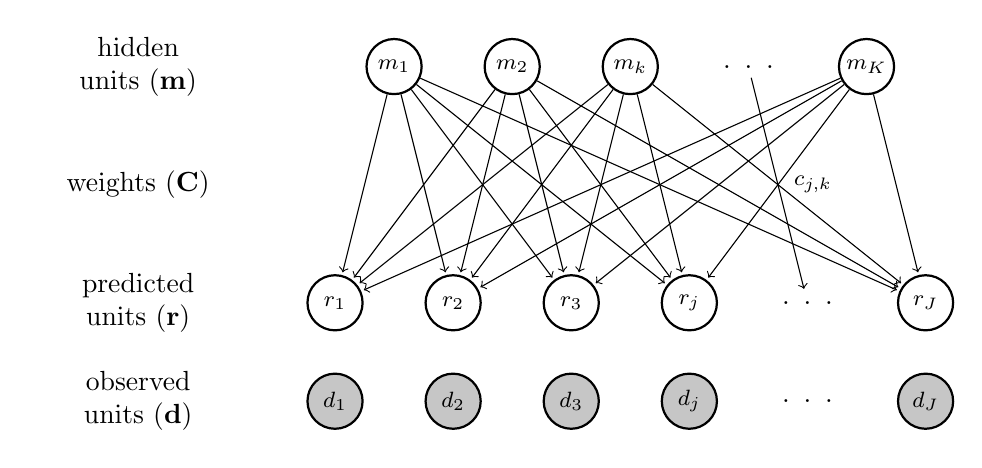
\begin{tikzpicture}[shorten >=1pt,->,draw=black!100]
	\def \rowtwoht{4.25cm}
	\def \weightlevel{2.75cm}
	\def \rowoneht{1.25cm}
	\def \basement{0cm}
	\tikzstyle{m-node}=[circle,draw=black!100,thick,inner sep=0pt,minimum size=7mm]
	\tikzstyle{r-node}=[circle,draw=black!100,thick,inner sep=0pt,minimum size=7mm]
	\tikzstyle{d-node}=[circle,draw=black!100,fill=gray!45,thick,inner sep=0pt,minimum size=7mm]
	\tikzstyle{dots}=[text width=5ex, text centered]
	\tikzstyle{annot}=[text width=17ex, text centered]
	% labels
	\node[annot] (hidden-layer) at (0cm,\rowtwoht) {hidden units ($\mathbf{m}$)};
	\node[annot] (weights) at (0cm,\weightlevel) {weights ($\mathbf{C}$)};
	\node[annot] (r-layer) at (0cm,\rowoneht) {predicted units ($\mathbf{r}$)};
	\node[annot] (d-layer) at (0cm,\basement) {observed units ($\mathbf{d}$)};
	
	\node[dots] 	(m3)	at (7.75cm,\rowtwoht)	 	{. . .};
	\node[dots] 	(r4) 	at (8.5cm,\rowoneht)   		{. . .};
	\node[dots] 	(d4) 	at (8.5cm,\basement)   		{. . .};
%	\node[annot] (d-label) (0, 0) {observed data vector};
	
	\footnotesize
	% hidden layer
	\node[m-node] 	(m0)	at (3.25cm,\rowtwoht)		{$m_1$};
	\node[m-node] 	(m1)	at (4.75cm,\rowtwoht)		{$m_2$};
	\node[m-node] 	(m2)	at (6.25cm,\rowtwoht)	 	{$m_k$};
	\node[m-node] 	(m4)	at (9.25cm,\rowtwoht)	 	{$m_K$};
	
	% reconstructed vector
	\node[r-node] 	(r0)	at (2.5cm,\rowoneht)		{$r_1$};
	\node[r-node] 	(r1)	at (4cm,\rowoneht)		{$r_2$};
	\node[r-node] 	(r2)	at (5.5cm,\rowoneht)	 	{$r_3$};
	\node[r-node] 	(r3)	at (7cm,\rowoneht) 		{$r_j$};
	\node[r-node] 	(r5) 	at (10cm,\rowoneht)   		{$r_J$};
	%\node[r-node] 	(r6) 	at (9.75cm,\rowoneht)   	{$r_J$};
	
	% data vector
	\node[d-node] 	(d0)	at (2.5cm,\basement)		{$d_1$};
	\node[d-node] 	(d1)	at (4cm,\basement)		{$d_2$};
	\node[d-node] 	(d2)	at (5.5cm,\basement)	 	{$d_3$};
	\node[d-node] 	(d3)	at (7cm,\basement) 		{$d_j$};
	\node[d-node] 	(d5) 	at (10cm,\basement)   		{$d_J$};
	%\node[d-node] 	(d6) 	at (9.75cm,\basement)   	{$d_J$};
	
	\path 
		(m0)	edge	node	{}	(r0)
		(m0)	edge	node	{}	(r1)
		(m0)	edge	node	{}	(r2)
		(m0)	edge	node	{}	(r3)
		%(m0)	edge	node	{}	(r4)
		(m0)	edge	node	{}	(r5)
		%(m0)	edge	node	{}	(r6)
		%
		(m1)	edge	node	{}	(r0)
		(m1)	edge	node	{}	(r1)
		(m1)	edge	node	{}	(r2)
		(m1)	edge	node	{}	(r3)
		%(m1)	edge	node	{}	(r4)
		(m1)	edge	node	{}	(r5)
		%(m1)	edge	node	{}	(r6)
		%
		(m2)	edge	node	{}	(r0)
		(m2)	edge	node	{}	(r1)
		(m2)	edge	node	{}	(r2)
		(m2)	edge	node	{}	(r3)
		(m2)	edge	node	{}	(r5)
		(m3)	edge	node[right=1mm]	{$c_{j,k}$}	(r4)
		%	
		(m4)	edge	node	{}	(r0)
		(m4)	edge	node	{}	(r1)
		(m4)	edge	node	{}	(r2)
		(m4)	edge	node	{}	(r3)
		(m4)	edge	node	{}	(r5);
		
\end{tikzpicture}
\end{center}
\caption{Architecture of a Multiple Cause Mixture Model (MCMM).} 
\label{fig:mcmm}
\end{figure*}

% \begin{figure}[htb]
% %\begin{minipage}{.3\textwidth}
% \begin{center}
% \small
% \begin{tikzpicture}[shorten >=1pt,->,draw=black!100]
% 	\def \rowtwoht{5cm}
% 	\def \weightstwo{3.75cm}
% 	\def \rowoneht{2.5cm}
% 	\def \weightsone{1.25cm}
% 	\def \basement{0cm}
% 	\tikzstyle{m-node}=[circle,draw=black!100,thick,inner sep=0pt,minimum size=7mm]
% 	\tikzstyle{r-node}=[circle,draw=black!100,thick,inner sep=0pt,minimum size=7mm]
% 	\tikzstyle{d-node}=[circle,draw=black!100,thick,inner sep=0pt,minimum size=7mm]
% 	\tikzstyle{dots}=[text width=5ex, text centered]
% 	\tikzstyle{annot}=[text width=20ex]
% 	% labels
% 	\node[annot] (hidden-layer) at (0cm,\rowoneht) {hidden layer $\mathbf{m}_{(k)}$};
% 	\node[annot] (weights) at (0cm,\weightsone) {weights $\mathbf{C}_{(k,j)}$};
% 	\node[annot] (r-layer) at (0cm,\basement) {surface layer $\mathbf{r}_{(j)}$};
	
% 	%\node[dots] 	(d4) 	at (8.5cm,\basement)   		{. . .};
% %	\node[annot] (d-label) (0, 0) {observed data vector};
	
% 	\footnotesize
% 	% hidden layer
% 	\node[m-node] 	(m0)	at (1.5cm,\rowoneht)		{$m_1$};
% 	\node[m-node] 	(m1)	at (2.5cm,\rowoneht)		{$m_2$};
% 	\node[dots] 	(m2)	at (3.5cm,\rowoneht)	 	{. . .};
% 	\node[m-node] 	(m3)	at (4.5cm,\rowoneht)	 	{$m_k$};
% 	\node[m-node] 	(m4)	at (5.5cm,\rowoneht)	 	{$m_K$};
	
% 	% data vector
% 	\node[dots] 	(r1) 	at (2.5cm,\basement)   		{. . .};
% 	\node[r-node] 	(r2)	at (3.5cm,\basement)		{$r_j$};
% 	\node[dots] 	(r3) 	at (4.5cm,\basement)   		{. . .};
	
% 	\path
% 		(m0)	edge	node	{}	(r2)
% 		(m1)	edge	node	{}	(r2)
% 		(m2)	edge	node	{}	(r2)
% 		(m3)	edge	node	{}	(r2)
% 		(m4)	edge	node	{}	(r2);
				
% \end{tikzpicture}
% \end{center}
% % \textit{Multiple Causes}
% \caption{A surface unit can have up to $K$ hidden causes. One cause is
%   sufficient to activate a unit.}
% %: an input layer ($\mathbf{d}$), a hidden layer ($\mathbf{m}$), and an output layer
% \label{fig:collider}
% \end{figure}
 
% \begin{figure}[htb]
% %\begin{minipage}{.3\textwidth}
% \begin{center}
% \small
% \begin{tikzpicture}[shorten >=1pt,->,draw=black!100]
% 	\def \rowtwoht{5cm}
% 	\def \weightstwo{3.75cm}
% 	\def \rowoneht{2.5cm}
% 	\def \weightsone{1.25cm}
% 	\def \basement{0cm}
% 	\tikzstyle{m-node}=[circle,draw=black!100,thick,inner sep=0pt,minimum size=7mm]
% 	\tikzstyle{r-node}=[circle,draw=black!100,thick,inner sep=0pt,minimum size=7mm]
% 	\tikzstyle{d-node}=[circle,draw=black!100,thick,inner sep=0pt,minimum size=7mm]
% 	\tikzstyle{dots}=[text width=5ex, text centered]
% 	\tikzstyle{annot}=[text width=20ex]
% 	% labels
% 	\node[annot] (hidden-layer) at (0cm,\rowoneht) {hidden layer $\mathbf{m}_{(k)}$};
% 	\node[annot] (weights) at (0cm,\weightsone) {weights $\mathbf{C}_{(k,j)}$};
% 	\node[annot] (r-layer) at (0cm,\basement) {surface layer $\mathbf{r}_{(j)}$};
	
% 	%\node[dots] 	(m2)	at (4.75cm,\rowoneht)	 	{. . .};
% 	%\node[dots] 	(d4) 	at (8.5cm,\basement)   		{. . .};
% %	\node[annot] (d-label) (0, 0) {observed data vector};
	
% 	\footnotesize
% 	% hidden layer
% 	%\node[m-node] 	(m0)	at (1.75cm,\rowoneht)		{$m_1$};
% 	%\node[m-node] 	(m1)	at (3.25cm,\rowoneht)		{$m_2$};
% 	\node[dots] 	(m0)	at (2.5cm,\rowoneht)		{. . .};
% 	\node[m-node] 	(m1)	at (3.5cm,\rowoneht)	 	{$m_k$};
% 	\node[dots] 	(m2)	at (4.5cm,\rowoneht)		{. . .};
% 	%\node[m-node] 	(m4)	at (7.75cm,\rowoneht)	 	{$m_K$};
	
% 	% data vector
% 	\node[r-node]	(r1) 	at (1.5cm,\basement)   		{$r_1$};
% 	\node[r-node] 	(r2)	at (2.5cm,\basement)		{$r_2$};
% 	\node[dots] 	(r3) 	at (3.5cm,\basement)   		{. . .};
% 	\node[r-node] 	(r4) 	at (4.5cm,\basement)   		{$r_j$};
% 	\node[r-node] 	(r5) 	at (5.5cm,\basement)   		{$r_J$};
	
% 	\path
% 		(m1)	edge	node	{}	(r1)
% 		(m1)	edge	node	{}	(r2)
% 		(m1)	edge	node	{}	(r3)
% 		(m1)	edge	node	{}	(r4)
% 		(m1)	edge	node	{}	(r5);
				
% \end{tikzpicture}
% \end{center}
% \caption{Conditionally-independent surface units}
% %: an input layer ($\mathbf{d}$), a hidden layer ($\mathbf{m}$), and an output layer
% \label{fig:cond-indep}
% \end{figure}

% \subsection{Autoencoder networks}
% \label{subsec:autoenc}

% The classical autoencoder is more widely known than the MCMM, so we
% will be using the former to frame our discussion of the latter.
% %as a reference point as we proceed to take a closer look at the MCMM. 
% Thus, in subsection
% \ref{subsec:autoenc} below, we summarize the major features of the classical autoencoder. 
% We then describe the MCMM in terms of these same features in \ref{subsec:mcmm-variant}, 
% noting similarities and crucial differences. We present a simple example MCMM in \ref{subsec:example}. 
% Finally, in \ref{subsec:mcmm-morph}, we show how MCMMs can be applied to the task of unsupervised morphological learning.

%
% Classical autoencoders
% %, shown in figure \ref{fig:autoencoder}, 
% consist of three layers of nodes: an input layer ($\mathbf{d}$), a
% hidden layer ($\mathbf{m}$), and a reconstruction (or output) layer
% ($\mathbf{r}$). It also has two weight matrices
% %$\mathbf{A}$ and $\mathbf{B}$, 
% linking the input units to the hidden units
% %($\mathbf{A}$) 
% and the hidden units to the reconstruction units.
% %($\mathbf{B}$).  
% The data and reconstruction layers are of the same size ($J$), while
% the hidden layer comprises fewer nodes ($K$), i.e., $K<J$.
%
% The input to the autoencoder is supplied by an $I \times J$ data
% matrix $\mathbf{D}$.  Each row in $\mathbf{d}_i$ in $\mathbf{D}$ is a
% distinct $J$-dimensional data point, and each column corresponds to
% one of the $J$ features that describe the dataset, so that the $j$th
% component in $\mathbf{d}_i$ specifies the value of the $j$th feature
% for the $i$th data point.  The reconstruction, or surface, layer
% contains the same
%
% Since an autoencoder learns by trying to reconstruct its input at its
% output layer, its output layer must have the same number of units as
% its input layer.  Thus, for each $J$-dimensional input vector
% $\mathbf{d_i}$, the network produces a corresponding $J$-dimensional
% reconstructed vector $\mathbf{r}_i$.  Each $\mathbf{r}_i$ constitutes
% a row in the $I \times J$ reconstruction matrix $\mathbf{R}$.
%
% When a data point is transmitted from the input layer through the network to the reconstruction layer, 
% it must on the way pass through a hidden layer $\mathbf{m}$ comprising $K$ nodes. 
% Importantly, $K < J$; i.e., the hidden layer has fewer nodes than the input and reconstruction layers.
% This smaller node count means that the hidden layer must find a
% conciser way to encode the data point before sending it on to the
% reconstruction layer.
%befothrough it en route to the reconstruction layer. 
% In effect, the hidden layer is forced to learn a compression scheme,
% i.e., a lower-dimensional encoding, for the dataset.
%$\mathbf{D}$.
% Thus, for every $J$-dimensional data point $\mathbf{d}_i$, the network
% learns a $K$-dimensional representation $\mathbf{m}_i$. Each
% $\mathbf{m}_i$ is a row in the $I \times K$ hidden-unit matrix
% $\mathbf{M}$.

% \begin{figure*}[htb]
% %\begin{minipage}{.3\textwidth}
% \begin{center}
% \small
% \begin{tikzpicture}[shorten >=1pt,->,draw=black!100]
% 	\def \rowtwoht{5cm}
% 	\def \weightstwo{3.75cm}
% 	\def \rowoneht{2.5cm}
% 	\def \weightsone{1.25cm}
% 	\def \basement{0cm}
% 	\tikzstyle{m-node}=[circle,draw=black!100,thick,inner sep=0pt,minimum size=7mm]
% 	\tikzstyle{r-node}=[circle,draw=black!100,thick,inner sep=0pt,minimum size=7mm]
% 	\tikzstyle{d-node}=[circle,draw=black!100,thick,inner sep=0pt,minimum size=7mm]
% 	\tikzstyle{dots}=[text width=5ex, text centered]
% 	\tikzstyle{annot}=[text width=17ex, text centered]
% 	% labels
% 	\node[annot] (r-layer) at (0cm,\rowtwoht) {reconstruction layer ($\mathbf{r}$)};
% 	\node[annot] (weights) at (0cm,\weightstwo) {weights ($\mathbf{B}$)};
% 	\node[annot] (hidden-layer) at (0cm,\rowoneht) {hidden layer ($\mathbf{m}$)};
% 	\node[annot] (weights) at (0cm,\weightsone) {weights ($\mathbf{A}$)};
% 	\node[annot] (d-layer) at (0cm,\basement) {input layer ($\mathbf{d}$)};
	
% 	\node[dots] 	(m3)	at (7.75cm,\rowoneht)	 	{. . .};
% 	\node[dots] 	(r4) 	at (8.5cm,\rowtwoht)   		{. . .};
% 	\node[dots] 	(d4) 	at (8.5cm,\basement)   		{. . .};
	
% 	\footnotesize
% 	% hidden layer
% 	\node[m-node] 	(m0)	at (3.25cm,\rowoneht)		{$m_1$};
% 	\node[m-node] 	(m1)	at (4.75cm,\rowoneht)		{$m_2$};
% 	\node[m-node] 	(m2)	at (6.25cm,\rowoneht)	 	{$m_k$};
% 	\node[m-node] 	(m4)	at (9.25cm,\rowoneht)	 	{$m_K$};
	
% 	% reconstructed vector
% 	\node[r-node] 	(r0)	at (2.5cm,\rowtwoht)		{$r_1$};
% 	\node[r-node] 	(r1)	at (4cm,\rowtwoht)		{$r_2$};
% 	\node[r-node] 	(r2)	at (5.5cm,\rowtwoht)	 	{$r_3$};
% 	\node[r-node] 	(r3)	at (7cm,\rowtwoht) 		{$r_j$};
% 	\node[r-node] 	(r5) 	at (10cm,\rowtwoht)   		{$r_J$};
% 	%\node[r-node] 	(r6) 	at (9.75cm,\rowoneht)   	{$r_J$};
	
% 	% data vector
% 	\node[d-node] 	(d0)	at (2.5cm,\basement)		{$d_1$};
% 	\node[d-node] 	(d1)	at (4cm,\basement)		{$d_2$};
% 	\node[d-node] 	(d2)	at (5.5cm,\basement)	 	{$d_3$};
% 	\node[d-node] 	(d3)	at (7cm,\basement) 		{$d_j$};
% 	\node[d-node] 	(d5) 	at (10cm,\basement)   		{$d_J$};
% 	%\node[d-node] 	(d6) 	at (9.75cm,\basement)   	{$d_J$};
	
% 	\path
% 		(d0)	edge	node	{}	(m0)
% 		(d0)	edge	node	{}	(m1)
% 		(d0)	edge	node	{}	(m2)
% 		%(d0)	edge	node	{}	(m3)
% 		(d0)	edge	node	{}	(m4)
% 		%	
% 		(d1)	edge	node	{}	(m0)
% 		(d1)	edge	node	{}	(m1)
% 		(d1)	edge	node	{}	(m2)
% 		%(d1)	edge	node	{}	(m3)
% 		(d1)	edge	node	{}	(m4)
% 		%
% 		(d2)	edge	node	{}	(m0)
% 		(d2)	edge	node	{}	(m1)
% 		(d2)	edge	node	{}	(m2)
% 		(d2)	edge	node	{}	(m4)
% 		%
% 		(d3)	edge	node	{}	(m0)
% 		(d3)	edge	node	{}	(m1)
% 		(d3)	edge	node	{}	(m2)
% 		(d3)	edge	node	{}	(m4)
% 		%
% 		(d4)	edge	node[right=2mm]	{$a_{j,k}$}	(m3)
% 		%
% 		(d5)	edge	node	{}	(m0)
% 		(d5)	edge	node	{}	(m1)
% 		(d5)	edge	node	{}	(m2)
% 		(d5)	edge	node	{}	(m4)
	 
% 		(m0)	edge	node	{}	(r0)
% 		(m0)	edge	node	{}	(r1)
% 		(m0)	edge	node	{}	(r2)
% 		(m0)	edge	node	{}	(r3)
% 		(m0)	edge	node	{}	(r5)

% 		(m1)	edge	node	{}	(r0)
% 		(m1)	edge	node	{}	(r1)
% 		(m1)	edge	node	{}	(r2)
% 		(m1)	edge	node	{}	(r3)
% 		(m1)	edge	node	{}	(r5)

% 		(m2)	edge	node	{}	(r0)
% 		(m2)	edge	node	{}	(r1)
% 		(m2)	edge	node	{}	(r2)
% 		(m2)	edge	node	{}	(r3)
% 		(m2)	edge	node	{}	(r5)

% 		(m3)	edge	node[right=3mm]	{$b_{k,j}$}	(r4)	
		
% 		(m4)	edge	node	{}	(r0)
% 		(m4)	edge	node	{}	(r1)
% 		(m4)	edge	node	{}	(r2)
% 		(m4)	edge	node	{}	(r3)
% 		(m4)	edge	node	{}	(r5);

		
% \end{tikzpicture}
% \end{center}
% \caption{In its classical form, an autoencoder network consists of three separate layers of nodes ($\mathbf{d}$, $\mathbf{m}$, and $\mathbf{r}$) and two layers of arcs. The matrices $\mathbf{A}$ and $\mathbf{B}$ define the weights on the arcs.}
% %: an input layer ($\mathbf{d}$), a hidden layer ($\mathbf{m}$), and an output layer
% \label{fig:autoencoder}
% \end{figure*}

% \marginpar{R1: how d and m are coupled? MD: I added a clause on
%   ``mediating ...'' }

%  (maybe more is needed in section~\ref{subsec:objfunc}?)}

% Like the classical autoencoder, the MCMM has a hidden layer
% $\mathbf{m}$ and a reconstruction layer $\mathbf{r}$.
% %, as in figure \ref{fig:mcmm}.  
% However,
%Unlike the classical autoencoder, the MCMM does not have an explicit
%data (or input) layer
%corresponding to the classical autoencoder's

The MCMM learns by comparing the reconstructed vector $\mathbf{r}_i$ 
to its corresponding original datapoint $\mathbf{d}_i$. The discrepancy between
the two is quantified by an \emph{objective function}. 
%(see section~\ref{mcmm-learning}) 
If there is a discrepancy, the values of the nodes in
$\mathbf{m}_i$ as well as the weights $\mathbf{C}$ are adjusted 
in order to reduce the discrepancy as much as possible.
%$\mathbf{d}$.  For MCMMs, $\mathbf{d}$ is an external standard to
%which $\mathbf{r}$ is compared via an error function
See section~\ref{mcmm-learning} for more on the learning process.
%(see section~\ref{subsec:objfunc}).
%
%Clusters]

Suppose data points $\mathbf{d}_u$ and $\mathbf{d}_v$ have some features in common.
Then, as the MCMM tries to reconstruct them in $\mathbf{r}_u$ and $\mathbf{r}_v$, respectively,
similarities will emerge between their respective hidden-layer vectors $\mathbf{m}_u$ and $\mathbf{m}_v$.
In particular, the vectors $\mathbf{m}_u$ and
$\mathbf{m}_v$ should come to share at least one active node, i.e., at least
one $k \in K$ such that $m_{u,k} = 1$ and $m_{v,k} = 1$.
% Hidden units represent the underlying properties responsible for
% regularities in the surface data. Such properties 
This can serve as a basis for clustering;
% When two data points share
% some underlying property, they will will also share at least one active hidden unit, namely whatever hidden  unit corresponds to the property in question.
% An autoencoder in this way functions as a clustering algorithm, and its hidden units act as indicators of cluster
% membership;
i.e., $m_{i,k}$ indicates whether $\mathbf{d}_i$ is a member of cluster $k$.
%$\mathbf{m}$ each indicating whether or not a data point is a member of a particular cluster.
%interpret $m_k$ as a cluster activity. 
%
% Because the MCMM has only two layers
% of nodes,
% %instead of three, 
% it needs only a single layer of connecting weights, the weight matrix
% $\mathbf{C}$.

% Suppose, for instance, that the second hidden unit is active for both $\mathbf{d}_u$ and $\mathbf{d}_v$ (i.e., $m_{u,2} = m_{v,2} = 1$). Then we can say that both data points belong to the second cluster.
% Now suppose that $\mathbf{m}_u$ and $\mathbf{m}_v$ are $[0,1,0,1,0]$ and $[0,1,0,0,0]$, respectively.
% In this case, $\mathbf{d}_u$ is a member of both the second and the fourth clusters, while $\mathbf{d}_v$ belongs solely to the second cluster. 
% Thus, for any row $i$ and column $k$ in the matrix $\mathbf{M}$, 
% $\mathbf{M}[i,k]$ is $1$ if and only if the $i$th data point belongs to the $k$th cluster, 
% and $0$ if and only if it does not.

%\paragraph{MCMM}

% This is a $J \times K$ matrix, since there are $K$ nodes in
% $\mathbf{m}$ and $J$ nodes in $\mathbf{r}$, and every $m_k$ must be
% linked to every $r_j$.

% \begin{figure*}[htb]
% %\begin{minipage}{.3\textwidth}
% \begin{center}
% \small
% \begin{tikzpicture}[shorten >=1pt,->,draw=black!100]
% 	\def \rowtwoht{4.25cm}
% 	\def \weightlevel{2.75cm}
% 	\def \rowoneht{1.25cm}
% 	\def \basement{0cm}
% 	\tikzstyle{m-node}=[circle,draw=black!100,thick,inner sep=0pt,minimum size=7mm]
% 	\tikzstyle{r-node}=[circle,draw=black!100,thick,inner sep=0pt,minimum size=7mm]
% 	\tikzstyle{d-node}=[circle,draw=black!100,fill=gray!45,thick,inner sep=0pt,minimum size=7mm]
% 	\tikzstyle{dots}=[text width=5ex, text centered]
% 	\tikzstyle{annot}=[text width=17ex, text centered]
% 	% labels
% 	\node[annot] (hidden-layer) at (0cm,\rowtwoht) {hidden units ($\mathbf{m}$)};
% 	\node[annot] (weights) at (0cm,\weightlevel) {weights ($\mathbf{C}$)};
% 	\node[annot] (r-layer) at (0cm,\rowoneht) {predicted units ($\mathbf{r}$)};
% 	\node[annot] (d-layer) at (0cm,\basement) {observed units ($\mathbf{d}$)};
	
% 	\node[dots] 	(m3)	at (7.75cm,\rowtwoht)	 	{. . .};
% 	\node[dots] 	(r4) 	at (8.5cm,\rowoneht)   		{. . .};
% 	\node[dots] 	(d4) 	at (8.5cm,\basement)   		{. . .};
% %	\node[annot] (d-label) (0, 0) {observed data vector};
	
% 	\footnotesize
% 	% hidden layer
% 	\node[m-node] 	(m0)	at (3.25cm,\rowtwoht)		{$m_1$};
% 	\node[m-node] 	(m1)	at (4.75cm,\rowtwoht)		{$m_2$};
% 	\node[m-node] 	(m2)	at (6.25cm,\rowtwoht)	 	{$m_k$};
% 	\node[m-node] 	(m4)	at (9.25cm,\rowtwoht)	 	{$m_K$};
	
% 	% reconstructed vector
% 	\node[r-node] 	(r0)	at (2.5cm,\rowoneht)		{$r_1$};
% 	\node[r-node] 	(r1)	at (4cm,\rowoneht)		{$r_2$};
% 	\node[r-node] 	(r2)	at (5.5cm,\rowoneht)	 	{$r_3$};
% 	\node[r-node] 	(r3)	at (7cm,\rowoneht) 		{$r_j$};
% 	\node[r-node] 	(r5) 	at (10cm,\rowoneht)   		{$r_J$};
% 	%\node[r-node] 	(r6) 	at (9.75cm,\rowoneht)   	{$r_J$};
	
% 	% data vector
% 	\node[d-node] 	(d0)	at (2.5cm,\basement)		{$d_1$};
% 	\node[d-node] 	(d1)	at (4cm,\basement)		{$d_2$};
% 	\node[d-node] 	(d2)	at (5.5cm,\basement)	 	{$d_3$};
% 	\node[d-node] 	(d3)	at (7cm,\basement) 		{$d_j$};
% 	\node[d-node] 	(d5) 	at (10cm,\basement)   		{$d_J$};
% 	%\node[d-node] 	(d6) 	at (9.75cm,\basement)   	{$d_J$};
	
% 	\path 
% 		(m0)	edge	node	{}	(r0)
% 		(m0)	edge	node	{}	(r1)
% 		(m0)	edge	node	{}	(r2)
% 		(m0)	edge	node	{}	(r3)
% 		%(m0)	edge	node	{}	(r4)
% 		(m0)	edge	node	{}	(r5)
% 		%(m0)	edge	node	{}	(r6)
% 		%
% 		(m1)	edge	node	{}	(r0)
% 		(m1)	edge	node	{}	(r1)
% 		(m1)	edge	node	{}	(r2)
% 		(m1)	edge	node	{}	(r3)
% 		%(m1)	edge	node	{}	(r4)
% 		(m1)	edge	node	{}	(r5)
% 		%(m1)	edge	node	{}	(r6)
% 		%
% 		(m2)	edge	node	{}	(r0)
% 		(m2)	edge	node	{}	(r1)
% 		(m2)	edge	node	{}	(r2)
% 		(m2)	edge	node	{}	(r3)
% 		(m2)	edge	node	{}	(r5)
% 		(m3)	edge	node[right=1mm]	{$c_{j,k}$}	(r4)
% 		%	
% 		(m4)	edge	node	{}	(r0)
% 		(m4)	edge	node	{}	(r1)
% 		(m4)	edge	node	{}	(r2)
% 		(m4)	edge	node	{}	(r3)
% 		(m4)	edge	node	{}	(r5);
		
% \end{tikzpicture}
% \end{center}
% \caption{Architecture of a Multiple Cause Mixture Model (MCMM).} 
% \label{fig:mcmm}
% \end{figure*}
\subsection{Mixing Function}
\label{sec:mixing-function}

% The degree of activity of a node 
% %(or unit)
% $y$ is determined by a \textit{mixing function}. A mixing function
% $\mu$ is essentially a voting rule \citep{saund:94}, i.e., a mapping
% from a set of input ``votes'' to a single output decision. Mixing
% functions differ in the specifics of this mapping
% ; i.e., different mixing functions have different ways of integrating
% the input votes.
% In a classical autoencoder, the mixing function is usually a composite function; given a node $y$, $\mu_y$ is the function ${net}_y$, i.e., $y$'s net ``raw" input, composed with the logistic sigmoid function $\sigma$. That is,
% %the logistic sigmoid function and ${net}$, the net ``raw" input to the node in question.
% %&, i.e., a weighted sum of $y$'s input signals. That is, 
% \begin{equation}\label{sigmoid}
% %\mu_y = \sigma_y \circ {net}_y = \sigma_y({net}_y)
% \mu_y = \sigma_y({net}_y) = \frac{1}{1 + e^{-{net}_y}}
% \end{equation}
% The function ${net}$ computes the inner product of two $N$-length vectors, namely a vector of input signals $\mathbf{x}$ and a vector of weights $\mathbf{w}$ such that $w_n$ is the weight associated with $x_n$, for $n = 1,2,\dots, N$. 
% \begin{equation}\label{weighted-sum}
% 	net(\mathbf{x}, \mathbf{w}) = \sum_{n=1}^N x_{n}w_{n}
% \end{equation}
% Note that ${net}$ is a mixing function in its own right; in particular, it is a linear mixing function, as it linearly combines the vectors $\mathbf{x}$ and $\mathbf{w}$. However, in the classical autoencoder's composite mixing function, the linear ${net}$ is followed by the nonlinear logistic sigmoid function $\sigma$, which  
% maps every output of $net$ to a value in $[0,1]$. Thus, the classical autoencoder's mixing function is ultimately nonlinear.

% Now, the classical autoencoder network has two layers of input-taking nodes:
% the hidden layer $\mathbf{m}$ and the reconstruction layer $\mathbf{r}$.
% %(see figure \ref{fig:autoencoder}). 
% Node activities propagate from the input layer to the hidden layer, and from the hidden layer to the reconstruction layer. 
% Each $m_k$ in the hidden layer $\mathbf{m}$ takes $J$ input signals, 
% one from each $d_j$ in $\mathbf{d}$.
% Each of these signals has a particular weight $a \in \mathbf{A}$, 
% so that $a_{j,k}$ is the weight on the signal from $d_j$ to $m_k$. 
% Plugging into equation $\eqref{weighted-sum}$ the input vector $\mathbf{d}$ and the weight vector 
% $\mathbf{a}_k$ gives us $net_k$, $m_k$'s net raw input.
% %which is the dot product of the vectors $\mathbf{d}$ and $\mathbf{a}_k$.
% \begin{equation}\label{weighted-sum-m}
% 	net_{k}(\mathbf{d}, \mathbf{a}_k) = \sum_{j=1}^J d_{j}a_{j,k}
% \end{equation}
% The value ${net}_k$ is then fed to the logistic sigmoid function $\eqref{sigmoid}$, which returns the activity (or excitation) of node $m_k$.
% %We write simply $m_k$ to signify the \emph{activity} of node $m_k$:
% \begin{equation}\label{sigmoid-m}
% 	m_{k} = \mu_k = \sigma({net}_{k}) = \frac{1}{1 + e^{-net_{k}}}
% \end{equation}
% The activities $\mathbf{m}$, i.e., the hidden layer's outputs, 
% become the inputs to the reconstruction layer $\mathbf{r}$. 
% Each $r_j$ in $\mathbf{r}$ takes $K$ input signals, each of the form $m_k b_{k,j}$ (for $k \in K$), where $b_{k,j}$ is a particular weight in the $J \times K$ weight matrix $\mathbf{B}$. 
% %Every link between $\mathbf{m}$ and $\mathbf{r}$ thus has a corresponding $b \in B$. 
% Let ${net}_j$ be the net raw input to the reconstruction node $r_j$. 
% This value is computed in the same way as ${net}_k$ in \eqref{weighted-sum-m} above, 
% only with different input and weight vectors;
% this time, the input vector is $\mathbf{m}$, and the weight vector is $\mathbf{b}_j$:
% \begin{equation}\label{weighted-sum-r}
% 	net_{j}(\mathbf{m}, \mathbf{b}_j) = \sum_{k=1}^K m_{k}b_{k,j}
% \end{equation}
% The activity of $r_j$ is then $\mu_j = \sigma(net_j)$:
% \begin{equation}\label{sigmoid-r}
% 	r_{j} = \mu_j = \sigma_j({net}_{j}) = \frac{1}{1 + e^{-net_{j}}}
% \end{equation}

% \paragraph{MCMM}

The mapping between the layer of hidden nodes $\mathbf{m}$ and the layer of surface nodes $\mathbf{r}$ is governed by a \emph{mixing function}, which is essentially
%The degree of activity of a node $y$
%(or unit)
%is determined by a \textit{mixing function},
%. A mixing function
%$\mu$ 
%is
a voting rule \citep{saund:94}; it maps from a set of
input ``votes'' to a single output decision.  The output decision is the activity (or inactivity) of a node $r_{ij}$ in the surface layer. Following \cite{saund:94}, we use the Noisy-Or function:
 \begin{equation}\label{eq:noisy-or}
 %r_{i,j} = 1 - \prod\limits_{k=0}^K (1 - m_{i,k} c_{j,k})
  r_{i,j} = 1 - \prod\limits_{k} (1 - m_{i,k} c_{j,k})
 \end{equation}
Note that the input to this function includes not only the hidden nodes $\mathbf{m}$, but also the \emph{weights} 
$\mathbf{c}_{j}$ on the hidden nodes. That is, the activity of the hidden node $m_k$ 
is weighted by the value $c_{jk}$.
A classical autoencoder also has a mixing function, though it is more commonly called an \textit{activation function} in autoencoders.
The most common activation function involves a simple weighted sum of the hidden layer $\mathbf{m}$'s activations. The entirely linear weighted sum is then passed to the logistic sigmoid function $\sigma$, which squashes the sum to a number between 0 and 1:
\begin{equation}\label{eq:sigmoid}
r_{i,j} = \sigma\Big(\sum_{k} m_{i,k} c_{j,k}\Big)
\end{equation}
Notice that both (\ref{eq:noisy-or}) and (\ref{eq:sigmoid}), have the same three primary components: the output (or surface node) $r_{i,j}$, the hidden layer of nodes $\mathbf{m}$, and a matrix of weights $\mathbf{C}$. Both are possible mixing functions.
%$r_{i,j}$ is a surface (or output) node, 
%$\sigma$ is the logistic sigmoid function, $m_{i,k}$ is a node in the hidden layer, and $c_{j,k}$ is its weight. 
%The sum $\sum_{k} m_k c_{j,k}$, then, is a weighted sum of the activities of the nodes in $\mathbf{m}$.
%of the input signals to surface (or output) node $r_{j}$'.
%Each input signal consists of a hidden-node activity $m_k$ multiplied by a weight 
%$c_{j,k}$. Thus, the classical autoencoder's mix

%of $y$'s individual input signals.

%Since $net_y$ is entirely
%linear, the weights have continuous values, i.e., values
%\emph{between} 0 and 1.  For linguistic processing, the
%interpretations of such values is unclear.
%
%In contrast, MCMM mixing functions encourage all parameters to
%converge to discrete values (0 or 1), which offer straightforward
%interpretations. \marginpar{Cite Bound Constrained Optimization for rational.}
%%, especially in the case of linguistic analysis.  This geare such that they encourage parameters to converge toward values that are clearly interpretable. 
%This property of MCMM mixing functions arises from their lack of any
%linear component.
%%``total'' nonlinearity (i.e., they have no linear component).
%Consider, for instance, the \textsc{noisy-or} function at the bottom
%of fig.~\ref{fig:example}, the mixing function used in this study,
%where multiplication encourages values to converge to 0 or 1.
%Following \cite{saund:94}, we instead use the Noisy-Or function:
% \begin{equation}\label{eq:noisy-or}
% %r_{i,j} = 1 - \prod\limits_{k=0}^K (1 - m_{i,k} c_{j,k})
%  r_{i,j} = 1 - \prod\limits_{k} (1 - m_{i,k} c_{j,k})
% \end{equation}
% Using multiplication, the \textsc{noisy-or} function encourages values
% to converge to 0 or 1.


% combines the products $m_{0}c_{0,j}, m_{1}c_{1,j}, ..., m_{K}c_{j,k}$ via multiplication rather than addition. 

% As long as at least one $m_kc_{j,k} = 1$, $r_{j}$ will be active, and
% $r_{j} = 0$ only if all products $m_kc_{j,k}$ are zero.

%Mixing functions differ in the mapping specifics.  
%MCMMs are distinguished by their propensity for learning
%configurations
%hidden-unit activations and weight configurations 
%with clear interpretations.

% In the classical autoencoder, the activity $\phi(net)$ of any node $y$
% is a function of its net raw input $net_y$, which is the weighted sum
% of $y$'s individual input signals.
% % (see \eqref{weighted-sum}). 
% The logistic sigmoid function $\phi$ then scales ${net}_y$ so that it
% falls within $[0,1]$.
% % \begin{align*}
% % r_{j} &= \sigma({net}_j) \\
% % &= \sigma\big(\sum_k b_{k,j} \cdot m_k \big) \\
% % &= \sigma \bigg(\sum_k b_{k,j} \cdot \sigma \big({net}_k \big) \bigg) \\
% % &= \sigma \bigg(\sum_k b_{k,j} \cdot \sigma \big(\sum_j a_{j,k} \cdot d_j \big) \bigg) \\
% % \end{align*}
% The activity of any given reconstruction node $r_j$ depends on two
% weight vectors, so that they may counteract each other,
% % not only on the weights $\mathbf{B}$, but also on the weights
% % $\mathbf{A}$.
% % %Moreover, $\mathbf{A}$ and $\mathbf{B}$ may differ.  
% % When $\mathbf{A} \ne \mathbf{B}$, the $\mathbf{B}$ weights can
% % counteract the effects of the $\mathbf{A}$ weights, 
% giving rise to unexpected activities among the $\mathbf{m}$ units and
% obscuring the relationships between the $\mathbf{m}$ and $\mathbf{r}$
% units.

%In a classical autoencoder, the activities of the reconstructed units $r_j$
%depend on the net effect of first weight layer, the hidden units $\mathbf{m}$,
%and the second layer of weights (which connect the hidden units to the reconstructed units).
%Since the two weight layers are likely going to differ, and they may conteract each other,
%giving rise to unexpected activities among the
%$\mathbf{m}$ units and obscuring the relationships between the
%$\mathbf{m}$ and $\mathbf{r}$ units.
%\marginpar{But is this a property of the mixing function?}
%of both the reconstructed units $r_j$ and the hidden units $m_k$
%depend on weights and can thus be manipulated only indirectly, by adjusting the weights.
%The hidden units depend on one layer of weights, while the reconstructed units depend on the net of effect of both weight layers, along with the activities of the hidden nodes. 
%depends on two layers of weights, which may counteract
%each other, resulting in unexpected activities among the
%$\mathbf{m}$ units and obscuring the relationships between the
%$\mathbf{m}$ and $\mathbf{r}$ units.
% The MCMM, in contrast, is designed with the purpose of providing a
% coherent causal explanation for regularities in surface data.  
%
%In contrast, because an MCMM has only one layer of weights, the activities of its
%hidden units must be manipulated directly. This direct approach is more conducive to arriving at parameters that have clear interpretations. 
%%Above all, an MCMM mixing function must be such that 
%%, providing for clear interpretations.  
%In the classical autoencoder, the terms $m_kc_{j,k}$
%%, k \in K$ 
%are combined linearly and then scaled by the logistic sigmoid function
%to fall within $[0,1]$. 
%But MCMMs employ mixing functions such that
%the combination of these terms is nonlinear from the start.
%%\textit{Why does this matter?} 
%This total nonlinearity encourages weights to converge toward discrete
%values. The ultimate decision is then based on multiple binary votes.
%%\textit{Why, then, is clipping necessary?}
%%
%%This is possible due to two factors: 1) 
%%\textit{Binary activities and weights.} 
%Both the weights and the hidden unit activities are constrained to
%stay in $[0,1]$, and at convergence all values---weights and hidden
%activities---should be either $0$ or $1$. 
%These binary values have clear interpretations.  2)
%\textit{Single layer of weights.} 
% Further, an MCMM has only one layer of weights: the activities of the
% hidden units are manipulated directly in response to the
% reconstruction error, providing for clearer interpretations.

% \textit{How so?} 

%\marginpar{Talk about ambiguity with the noisy-or function?}

%Moreover, MCMMs can use other mixing functions.
% The classical autoencoder's activation function $\sigma({net}_y)$ is
% one possible mixing function, for it indeed takes the $K$ distinct
% input signals to node $y$ and yields a single activity value.
% However, 
%For example, 
%As for the specific mixing functions, ones like
%%Saund points out that
%% $\sigma({net}_y)$ is not well-suited to the purpose of coherently
%% distinguishing causes from non-causes because $net_y$ is additive
%% rather than multiplicative \citep{saund:94}.  By contrast, the
%the \textsc{noisy-or} mixing function are preferred, as these are
%multiplicative, as in (\ref{eq:noisy-or}).  As long as at least one
%$m_kc_{j,k} = 1$,
%%(where $k = 0,1,\dots,K$),
%$r_{j}$ will be active, and $r_{j} = 0$ only if all products
%$m_kc_{j,k}$ are zero.  
%%Although there are possibilities, 
%We use the \textsc{noisy-or} mixing function in our experiments.

%\marginpar{MD: Check indices (starting at 0 or 1) throughout}
%\begin{equation}
%\label{eq:noisy-or}
%r_{j} = 1 - \prod_{k=0}^K (1 - m_kc_{j,k})
%% r_{j} &= 1 - (1 - m_0c_{0,j}) \times (1 - m_1c_{1,j}) \times (1 - m_2c_{2,j}) \\
%% &= 1 - (1 - 0) \times (1 - 0) \times (1 - 1) \\ 
%% &= 1 - 1 \times 1 \times 0 \\
%% &= 1
%\end{equation}
%Notice that $m_kc_{j,k} = 1$ only if both $m_k = 1$ and $c_{j,k} = 1$.
% On the other hand, with sigmoid squashing, $\sigma({net}_j)$ is never
% truly zero; it just gets infinitely close to zero.  And
% $\sigma({net}_j)$ will be close to $1$ as long as ${net}_j = \sum_K
% m_k c_{j,k}$ is sufficiently large.  There are an infinite number of
% valuations for $\mathbf{m}$ and $\mathbf{c}_{j}$ that could give rise
% to a sufficiently large ${net}_j$.
%
% The function ${net}$ is an example of a linear mixing
% function. However, the autoencoder's mixing function is made nonlinear
% by $\phi({net}_y)$, which ``squashes" $net_y$ to fall within $[0,1]$.

\subsection{Learning}
\label{mcmm-learning}
%\label{autoencoder-learning}

% A data compression scheme is useful only to the extent that it allows
% for the recovery of the source data from the compressed
% representations. In autoencoder terms, this means that 

%The reconstruction layer attempts to
%decode the hidden layer's representations and
In both the classical autoencoder and the MCMM, learning occurs as a
result of the algorithm's search for an optimal valuation of key variables (e.g., weights), 
i.e., a valuation that minimizes %or maximizes an the
%\emph{reconstruction error} $E$, 
the discrepancy between
reconstructed and original data points.  The search is conducted
via %some method of 
numerical optimization; we use the nonlinear conjugate gradient method.
%gradient-based technique, e.g., gradient descent or
%the conjugate gradient method.
%
Our objective function is a simple error function, namely the
normalized sum of squares error:
\begin{equation}
E = \frac{1}{I \times J} \sum_{i} \sum_{j} {(r_{i,j} - d_{i,j})}^2
\end{equation}
 where $I \times J$ is the total number of features in the dataset.
The MCMM's task is to minimize this function by adjusting the
 values in $\mathbf{M}$ and $\mathbf{C}$, where
 %$I \times $ matrix $\mathbf{M}$ and the $J \times K$ matrix $\mathbf{C}$.
$\mathbf{M}$ is the $I \times K$ matrix that
% of dimensions $I \times K$,
encodes each data point's cluster-activity vector, 
and $\mathbf{C}$ is the $J \times K$ matrix that
%, of dimensions $J \times K$, 
encodes the weights between $\mathbf{m}_i$ and $\mathbf{r}_i$ for every $i \in I$ (see fig.~\ref{fig:example}). 
%$\mathbf{C}$ can also be interpreted as encoding the cluster centroids 
%(the clusters' ``average'' data points).
%Each column in $\mathbf{C}$ is in effect a feature vector; the $k^{\mathrm{th}}$ column is 
%the $k^{\mathrm{th}}$ cluster's average feature vector.
% \begin{align*}
% 	% E &= \frac{1}{I} \sum_{i} e_{i} \\
% 	% e_{i} &= \frac{1}{J} \sum_{j} {(r_{i,j} - d_{i,j})}^2
% 	E &= \frac{1}{I \times J} \sum_{i} \sum_{j} {(r_{i,j} - d_{i,j})}^2
% \end{align*}
% %\marginpar{Rationale for normalized SSE?} 
% which is minimized.
% rather than maximized.  
%Thus, instead of gradient ascent, we use gradient descent to find the
%optimal parameters.

%; our techniques are described in section~\ref{subsec:objfunc}.
% There are a number of possibilities regarding the particular error
% function and gradient-based technique. We describe our choices in
% section~\ref{subsec:objfunc}.
% Any information loss in the compression will result in reconstructed
% vectors that differ from the original data points.  This is called
%the \emph{reconstruction error} is measured by some error function
%$err$, such as the
%%.  A typical error function is 
%the sum of squared error ($err_i = \sum_{j}{(d_{i,j} -
%  r_{i,j})}^2$). The global reconstruction error $E$, for the whole
%dataset, is the sum of all $err_i$.
%% over $i \in I$.
%%
%To discover a compression scheme with a minimal $E$, autoencoders
%use gradient-based search techniques, e.g., gradient descent or the
%conjugate gradient method.  We describe our error function in
%section~\ref{subsec:objfunc}.

% The autoencoder's goal is to discover a compression scheme that causes a minimal $E$, 
% and since $E$ is ultimately a function of $\mathbf{A}$ and $\mathbf{B}$, 
% this task reduces to finding the valuations for $\mathbf{A}$ and $\mathbf{B}$ that minimize $E(\mathbf{A},\mathbf{B}$). To this end, autoencoders use gradient-based search techniques, e.g., gradient descent or the conjugate gradient method. In the remainder of this section, we provide a very general description of an autoencoder's weight updating process. The details, especially the specific form of the weight-update function, depend on the particular gradient-based technique used. 

% Taking as input the data points $\mathbf{d}_i \in \mathbf{D}$, the network yields a reconstructed vector $\mathbf{r}_i$ for each individual $\mathbf{d}_i$. Because $\mathbf{D}$ contains $I$ data points, one epoch (i.e., one cycle through the dataset) is complete after $I$ iterations, whereupon ${E}(\mathbf{A}, \mathbf{B})$ is calculated, and each weight in $\mathbf{A}$ and $\mathbf{B}$ is adjusted in a way that furthers the descent of $E$ toward a minimum. 
% In particular, the algorithm adds to each 
% $b_{k,j} \in \mathbf{B}$ a quantity proportional to the negative gradient of 
% $E$ at $b_{k,j}$, or $-\frac{\partial E}{\partial b_{k,j}}$. 
% It similarly adds to each $a_{j,k} \in \mathbf{A}$
% a quantity proportional to the negative gradient of $E$ at $a_{j,k}$,
% or $-\frac{\partial E}{\partial a_{j,k}}$.
% These weight updates serve to improve the network's compression model, so that each successive epoch yields a smaller reconstruction error than the preceding epoch.
% The succession of epochs continues until $E$ falls below some small predesignated value.


% \subsection{The MCMM as an autoencoder variant}
% \label{subsec:mcmm-variant}

%\subsubsection{Architecture}
% Like the classical autoencoder, the MCMM has a hidden layer $\mathbf{m}$ and a reconstruction layer $\mathbf{r}$, as illustrated in figure \ref{fig:mcmm}. 
% However, the MCMM does not have an explicit
% data (or input) layer corresponding to the classical autoencoder's $\mathbf{d}$.
% Because the MCMM has only a two layers of nodes instead of three, it needs only a single layer of connecting weights, namely the weight matrix $\mathbf{C}$. This is a $J \times K$ matrix,
% since there are $K$ nodes in $\mathbf{m}$ and $J$ nodes in $\mathbf{r}$,
% and every $m_k$ must be linked to every $r_j$.

%\subsubsection{Mixing Function}
% MCMMs are distinguished by their propensity for learning hidden-unit activations and weight configurations that have clear interpretations.

% In the classical autoencoder, the activity $\phi(net)$ of any node $y$ is a
% function of its net raw input $net_y$, which is the weighted sum of $y$'s
% individual input signals (see \eqref{weighted-sum}). 
% The logistic sigmoid function $\phi$ then scales ${net}_y$ so that it falls within $[0,1]$.

% \begin{align*}
% r_{j} &= \sigma({net}_j) \\
% &= \sigma\big(\sum_k b_{k,j} \cdot m_k \big) \\
% &= \sigma \bigg(\sum_k b_{k,j} \cdot \sigma \big({net}_k \big) \bigg) \\
% &= \sigma \bigg(\sum_k b_{k,j} \cdot \sigma \big(\sum_j a_{j,k} \cdot d_j \big) \bigg) \\
% \end{align*}
% The activity of any given reconstruction node $r_j$ depends not only on the weights $\mathbf{B}$, but also on the weights $\mathbf{A}$.
% Moreover, $\mathbf{A}$ and $\mathbf{B}$ may differ.
% When $\mathbf{A} \ne \mathbf{B}$, the $\mathbf{B}$ weights can counteract the effects of the $\mathbf{A}$ weights, giving rise to unexpected activities among the $\mathbf{m}$ units and obscuring the  
% relationships between the $\mathbf{m}$ units and the $\mathbf{r}$ units.

% The MCMM, in contrast, is designed with the express purpose of providing a coherent causal explanation for regularities in surface data.
% What makes this possible?
% \begin{itemize} 
% \item \textit{Binary activities and weights.} Both the weights and the hidden unit activities are constrained to stay in $[0,1]$. At convergence, moreover, all values---both weights and hidden activities---should be either $0$ or $1$. \textit{Why is this important?} Binary values, i.e., \textsc{true} and \textsc{false}, have clear interpretations.
% \item \textit{Single layer of weights.} An MCMM has only one layer of weights. \textit{Why is this important?} The activities of the hidden units are manipulated directly in response to the reconstruction error.
% \item 
% \textit{How so?} In the classical autoencoder, the terms $m_kc_{j,k}, k \in K$ are combined linearly prior to sigmoid squashing. But MCMMs employ mixing functions such that the combination of these terms is nonlinear from the start. \textit{Why does this matter?} This ``total" nonlinearity encourages (?) weights to converge toward discrete values. The ultimate decision is then based on multiple discrete, either-or votes.
% \textit{Why, then, is clipping necessary?}
% \end{itemize}
% Moreover, they use mixing functions that 
% The classical autoencoder's activation function $\sigma({net}_y)$ is one possible mixing function,
% for it indeed takes the $K$ distinct input signals to node $y$ and yields a single activity value.
% However, as Saund points out, $\sigma({net}_y)$ is not well suited to the purpose of coherently distinguishing causes from non-causes. This is because $net_y$ is additive rather than multiplicative. Noisy-or is multiplicative:
% \begin{align*}
% r_{j} &= 1 - (1 - m_0c_{0,j}) \times (1 - m_1c_{1,j}) \times (1 - m_2c_{2,j}) \\
% &= 1 - (1 - 0) \times (1 - 0) \times (1 - 1) \\ 
% &= 1 - 1 \times 1 \times 0 \\
% &= 1
% \end{align*}
% As long as at least one $m_kc_{j,k} = 1$ (where $k = 0,1,\dots,K$), $r_{j}$ will be active,
% and $r_{j} = 0$ only if all products $m_kc_{j,k}$ are zero.
% Notice that $m_kc_{j,k} = 1$ only if both $m_k = 1$ and $c_{j,k} = 1$.
% On the other hand, with sigmoid squashing, $\sigma({net}_j)$ is never truly zero; it just gets infinitely close to zero.
% And $\sigma({net}_j)$ will be close to $1$ as long as ${net}_j = \sum_K m_k c_{j,k}$ is sufficiently large. 
% There are an infinite number of valuations for $\mathbf{m}$ and $\mathbf{c}_{j}$ that could give rise to a sufficiently large ${net}_j$.

% The function ${net}$ is an example of a linear mixing function. However, the autoencoder's mixing function
% is made nonlinear by $\phi({net}_y)$, which ``squashes" $net_y$ to fall within $[0,1]$.

%\subsubsection{Learning}
%\label{mcmm-learning}

%\paragraph{MCMM}

%\marginpar{MD: In fig.~\ref{fig:example}, we use $\mathbf{M}$, but
%  in previous figures we use $\mathbf{m}$.  Also, why is it sometimes
%  $\mathbf{m_k}$ and sometimes $\mathbf{m_{i,k}}$?  ($i$ refers to the
%  $i^{\mathrm{th}}$ word?)}

The MCMM's learning process is similar to Expectation Maximization
(EM) in that at any given time it is holding one set of variables 
fixed while optimizing the other set. We thus have two functions, \textsc{Optimize-M}
and \textsc{Optimize-C}, which take turns optimizing their respective matrices.
% However, if the algorithm is to optimize $\mathbf{M}$, it must first
% know $\mathbf{C}$, and vice versa.  Therefore, the algorithm can only
% focus on matrix at time, optimizing the one while holding the other
% fixed.
% The learning process consists of two distinct optimization
% functions:
%, \textsc{Optimize-M} and \textsc{Optimize-C}.
%\begin{description}
%\item[
% \textsc{Optimize-M} holds $\mathbf{C}$ fixed in order to optimize the
% cluster activity vectors in $\mathbf{M}$, while \textsc{Optimize-C}
% holds $\mathbf{M}$ fixed in order to optimize the cluster centroids in
% $\mathbf{C}$.
%\end{description}

The function \textsc{Optimize-M} visits each of the $I$ cluster-activity vectors $\mathbf{m}_i$ in
$\mathbf{M}$, optimizing each one separately.
%, one at a time.
%in $\mathbf{M}$, 
For each $\mathbf{m}_i$, \textsc{Optimize-M} enters an optimization 
loop over its $K$ components, adjusting each 
$m_{i,k}$ by a
quantity proportional to the negative gradient of $E$ at $m_{i,k}$.
%(details omitted for space reasons). 
This loop repeats until $E$
ceases to decrease significantly,
%with respect to $m_{i,k}$,
%(i.e., $E$ stops decreasing significantly),
whereupon \textsc{Optimize-M} proceeds to the next $\mathbf{m}_i$.  
% \textsc{Optimize-M} is thus a succession of $I$ optimization loops, one
% loop for each cluster activity vector $\mathbf{m}_i$. 
%(i.e., for each of the $i$ data points).

The function \textsc{Optimize-C} consists of a single optimization loop over the 
entire matrix
$\mathbf{C}$. Each %component 
$c_{j,k}$ is adjusted by a quantity
proportional to the negative gradient of $E$ at $c_{j,k}$.
%, or $-\frac{\partial E}{\partial c_{j,k}}$.
%(in the case of gradient descent).  
%Since $E$ is simply
%$\sum_i e_i$, i.e., the sum of the errors of the individual data-point
%reconstructions, $-\frac{\partial E}{\partial c_{j,k}} = -\sum_i
%\frac{\partial e_i}{\partial c_{j,k}}$.  Thus, the adjustment to each
%$c_{j,k}$ takes into account the error of each reconstructed vector
%$\mathbf{r}_i$ in $\mathbf{R}$. However,
Unlike \textsc{Optimize-M}, which comprises $I$ separate optimization
loops, \textsc{Optimize-C} consists of just one, 
%optimizing the $\mathbf{C}$ matrix as a whole.  
When each of its $J \times K$
components has been adjusted, one round of updates to $\mathbf{C}$ is
complete.  $E$ is reassessed only between completed rounds of
updates. If the change in $E$ remains significant, another round begins.  

% \marginpar{MD: I wasn't sure whether I should include
%   somehting about Armijo conditions. TM: We probably don't have to go into that.}
%  (We use a non-linear conjugate
%gradient method for the update rules, but, again, details are omitted
%for space reasons. 

Both \textsc{Optimize-M} and \textsc{Optimize-C} are enclosed within 
an ``alternation loop" 
that alternates between the two functions, holding $\mathbf{C}$ fixed
during \textsc{Optimize-M}, and vice versa.
%$\mathbf{M}$ fixed during \textsc{Optimize-C}. 
This alternation continues until $E$ cannot be decreased further. At
this point, an ``outer loop''
%(containing the alternating loop) 
splits the cluster which contributes the most to the error, adds one
to the cluster count $K$, and restarts the alternation loop. The outer loop
repeats until it reaches an overall stopping criterion, e.g., $E = 0$.
%; otherwise, the function terminates.
 
The optimization task is subject to the constraint %$0 le m_{i,k} ge 1$
that no value in $\mathbf{M}$ or $\mathbf{C}$ may exceed 1 or fall below 0. In other words,
it is a task of bound constrained optimization. Thus, whenever a value in either $\mathbf{M}$ or $\mathbf{C}$ is about
to fall below 0, it is set to 0. Likewise, whenever a value is about to exceed 1, it is set to 1
\citep{ni:yuan:1997}.
 %It repeatedly iterates over the $J \times K$ components of $\mathbf{C}$, stopping only when it finds a local minimum of $E$ is
  
%What is the inner loop and what is the outer loop?
%There are actually two inner loops: Opt-M is immediately followed by Opt-C. These two are encapsulated within a larger outer loop.
%What is the stopping criterion for the inner loop? What happens when this criterion is met?
%What is the stopping criterion for the outer loop?
%Cluster Splitting. Where does this enter the narrative?
%At this point, the algorithm then finds the worst cluster among the currently existing clusters and splits it, thereby increasing the cluster count $K$ by one.

\subsection{A Simple MCMM Example}
\label{subsec:example}

Fig.~\ref{fig:example} shows an example of an MCMM for two data points (i.e., $I = 2$).
% is given in fig.~\ref{fig:example}, for $I=2$,
%i.e., 2 data points. , each with 3 features.
%
%Together, 
The hidden cluster activities $\mathbf{M}$, the weights $\mathbf{C}$,
and the mixing function $r$ constitute a model that reproduces the
observed data points $\mathbf{D}$.
%
%\marginpar{MD: I don't quite understand the ``center vector''
  %statement}
%
The nodes $m_{i,k}$ represent cluster activities; if $m_{1,2} = 1$,
for instance, the second cluster is active for $\mathbf{d}_1$ (i.e.,
$\mathbf{d}_1$ is a member of cluster 2).
%
Note that the $J \times K$ weight matrix $\mathbf{C}$ is the same for
all data points, and
%
% For each data point, the arcs emanating from cluster
% 1 and cluster 2 represent the components of $\mathbf{C}$'s first and
% second rows, respectively. The $k$th row in $\mathbf{C}$ is thus
% uniquely associated with the $k$th cluster. Moreover, 
%
the $k^{\mathrm{th}}$ row in $\mathbf{C}$ can be seen as the $k^{\mathrm{th}}$
cluster's ``average" vector: the $j^{\mathrm{th}}$ component in
$\mathbf{c}_k$ is 1 only if all data points in cluster $k$ have
1 at feature $j$.
%the $k^{\mathrm{th}}$ row of $\mathbf{C}$ is in effect
%the center vector of the $k^{\mathrm{th}}$ hidden cluster.
%
%In the figure, 

%\begin{figure}[htb!]
%\usetikzlibrary{positioning}
%%\begin{minipage}{.3\textwidth}
%\begin{center}
%%\subfigure[Learning in Progress]{
%\begin{tikzpicture}[shorten >=1pt,->,draw=black!100, scale=0.85]
%	\footnotesize
%%	\def \attic{5.95cm}
%%	\def \rowtwoht{5.4cm}
%%	\def \weightlevel{3.9cm}
%%	\def \rowoneht{2.4cm}
%%	\def \basement{1.8cm}
%%	\def \data{1cm}
%%	\def \china{0cm}
%
%	\def \attic{5.4cm}
%	\def \rowtwoht{4.8cm}
%	\def \weightlevel{3.6cm}
%	\def \rowoneht{2.4cm}
%	\def \basement{1.8cm}
%	\def \data{1cm}
%	\def \china{0cm}
%		
%	\tikzstyle{m-node}=[circle,draw=black!100,thick,inner sep=0pt,minimum size=6mm]
%	\tikzstyle{r-node}=[circle,draw=black!100,thick,inner sep=0pt,minimum size=6mm]
%	\tikzstyle{d-node}=[circle,draw=black!100,fill=gray!45,thick,inner sep=0pt,minimum size=6mm]
%	%\tikzstyle{dots}=[text width=5ex, text centered]
%	\tikzstyle{annot}=[text width=2.5em]
%	% labels
%	\tikzstyle{label}=[text width=2.5em, text centered]
%	\tikzstyle{formula}=[text width=30em, text centered]
%	
%	\scriptsize
%	\node[annot] (hidden-layer) at (0cm,\rowtwoht) {$\mathbf{M}_{(i,k)}$};
%	\node[annot] (weights) at (0cm,\weightlevel) {$\mathbf{C}_{(j,k)}$};
%	\node[annot] (r-layer) at (0cm,\rowoneht) {$\mathbf{R}_{(i,j)}$};
%	
%	% hidden layer
%	\scriptsize
%	\node[m-node] 	(ma00)	at (1.45cm,\rowtwoht)		{$.2$};
%	\node[m-node] 	(ma01)	at (3.35cm,\rowtwoht)		{$.9$};
%	\node[m-node] 	(ma10)	at (5.55cm,\rowtwoht) 	{$.8$};
%	\node[m-node] 	(ma11)	at (7.45cm,\rowtwoht)	 	{$.1$};
%	% \node[m-node] 	(m20)	at (9.65cm,\rowtwoht) 	{$.8$};
%	% \node[m-node] 	(m21)	at (11.55cm,\rowtwoht)	 	{$.9$};
%	
%	%\footnotesize
%	\node[label]	(ml00) 	at (1.45cm,\attic)		{$m_{1,1}$}; %1.75 -> 1.45
%	\node[label]	(ml01) 	at (3.35cm,\attic)		{$m_{1,2}$}; %3.05 -> 3.35
%	\node[label] 	(ml10)	at (5.55cm,\attic) 	{$m_{2,1}$};     %5.85 -> 5.55
%	\node[label] 	(ml11)	at (7.45cm,\attic)	 	{$m_{2,2}$}; %7.15 -> 7.45
%	% \node[label] 	(ml20)	at (9.65cm,\attic) 	{$m_{3,1}$};     %9.95 -> 9.65
%	% \node[label] 	(ml21)	at (11.55cm,\attic)	 	{$m_{3,2}$}; %11.25 -> 11.55
%	
%	\scriptsize
%	\node[r-node] 	(ra00)	at (1.1cm,\rowoneht)		{$.24$};
%	\node[r-node] 	(ra01)	at (2.4cm,\rowoneht)		{$.81$};
%	\node[r-node] 	(ra02)	at (3.7cm,\rowoneht)	 	{$.23$};
%	
%	\node[r-node] 	(ra10)	at (5.2cm,\rowoneht) 		{$.68$};
%	\node[r-node] 	(ra11) 	at (6.5cm,\rowoneht)   	{$.16$};
%	\node[r-node] 	(ra12)	at (7.8cm,\rowoneht)		{$.76$};
%	
%	% \node[r-node] 	(r20) 	at (9.3cm,\rowoneht)  		{$.71$};
%	% \node[r-node] 	(r21)	at (10.6cm,\rowoneht) 		{$.83$};
%	% \node[r-node] 	(r22) 	at (11.9cm,\rowoneht)   	{$.77$};
%	
%	\node[label] 	(rl00)	at (1.1cm,\basement)		{$r_{1,1}$};
%	\node[label] 	(rl01)	at (2.4cm,\basement)		{$r_{1,2}$};
%	\node[label] 	(rl02)	at (3.7cm,\basement)	 	{$r_{1,3}$};
%	
%	\node[label] 	(rl10)	at (5.2cm,\basement) 		{$r_{2,1}$};
%	\node[label] 	(rl11) 	at (6.5cm,\basement)   	{$r_{2,2}$};
%	\node[label] 	(rl12)	at (7.8cm,\basement)		{$r_{2,3}$};
%	
%%	\node[label] 	(rl20) 	at (9.3cm,\basement)  		{$r_{3,1}$};
%%	\node[label] 	(rl21)	at (10.6cm,\basement) 		{$r_{3,2}$};
%%	\node[label] 	(rl22) 	at (11.9cm,\basement)   	{$r_{3,3}$};
%
%	\draw[-] (4.45cm, \attic+1.5mm) -- (4.45cm, \basement-1.5mm);
%%	\draw[-] (8.55cm, \attic+1.5mm) -- (8.55cm, \basement-1.5mm);
%
%	\scriptsize
%	\path
%		(ma00)	edge	node [left]	{$.85$} (ra00)
%		(ma00)	edge	node [left,xshift=-1mm,yshift=3mm]	{$.1$}	(ra01)
%		(ma00)	edge	node [left,xshift=-1mm,yshift=8mm]	{$.95$}	(ra02)
%
%		(ma01)	edge	node [right,xshift=3mm,yshift=8mm]	{$.1$}	(ra00)
%		(ma01)	edge	node [right,xshift=1mm,yshift=3mm]	{$.9$}	(ra01)
%		(ma01)	edge	node [right]	{$.05$} (ra02)
%		%
%		(ma10)	edge	node [left] {$.85$} (ra10)
%		(ma10)	edge	node [left,xshift=-1mm,yshift=3mm]	{$.1$}	(ra11)
%		(ma10)	edge	node [left,xshift=-1mm,yshift=8mm] {$.95$}	(ra12)
%		
%		(ma11)	edge	node [right,xshift=3mm,yshift=8mm]	{$.1$}	(ra10)
%		(ma11)	edge	node [right,xshift=1mm,yshift=3mm]	{$.9$}	(ra11)
%		(ma11)	edge	node [right]	{$.05$} (ra12);
%		%
		% (m20)	edge	node [left]	{$.85$}	(r20)
		% (m20)	edge	node [left,xshift=-1mm,yshift=4mm]	{$.1$}	(r21)
		% (m20)	edge	node [left,xshift=-1mm,yshift=10mm]	{$.95$} (r22)
		
		% (m21)	edge	node [right,xshift=3mm,yshift=10mm]		{$.1$}	(r20)
		% (m21)	edge	node [right,xshift=1mm,yshift=4mm]{$.9$}	(r21)
		% (m21)	edge	node [right]	{$.05$}	(r22);		
		
%\end{tikzpicture}
%\label{fig:example:fig1}
%\caption{A simple MCMM example} % showing learning in progress}
%\label{fig:example:fig1}
%\end{center}
%\end{figure}

\begin{figure}[htb!]
\usetikzlibrary{positioning}
\begin{center}
\subfigure[Observed Data]{
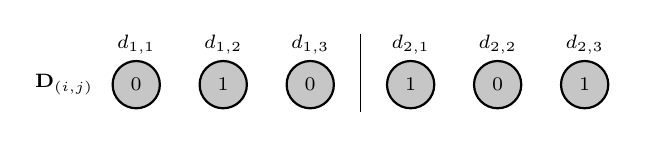
\begin{tikzpicture}[shorten >=1pt,->,draw=black!100, scale=0.85]
	\scriptsize
	\tikzstyle{label}=[text width=3em, text centered]
	\tikzstyle{annot}=[text width=2.5em]
	\tikzstyle{d-node}=[circle,draw=black!100,fill=gray!45,thick,inner sep=0pt,minimum size=6mm]
	
	\def \china{0.6cm}
	\def \data{0cm}
	
	\node[annot] (d-layer) at (0cm,\data) {$\mathbf{D}_{(i,j)}$};
	\draw[-] (4.45cm, \china+1.5mm) -- (4.45cm, \data-4.5mm);
%	\draw[-] (8.55cm, \china+1.5mm) -- (8.55cm, \data-4.5mm);
	%\draw[-] (-1cm, \china+.5cm) -- (13cm, \china+.5cm);
	%\draw[-] (-1cm, \data-.5cm) -- (13cm, \data-.5cm);
	
	\node[label] 	(dl00)	at (1.1cm,\china)		{$d_{1,1}$};
	\node[label] 	(dl01)	at (2.4cm,\china)		{$d_{1,2}$};
	\node[label] 	(dl02)	at (3.7cm,\china)	 	{$d_{1,3}$};
	
	\node[label] 	(dl10)	at (5.2cm,\china) 		{$d_{2,1}$};
	\node[label] 	(dl11) 	at (6.5cm,\china)   	{$d_{2,2}$};
	\node[label] 	(dl12)	at (7.8cm,\china)		{$d_{2,3}$};
	
	% \node[label] 	(dl20) 	at (9.3cm,\china)  		{$d_{3,1}$};
	% \node[label] 	(dl21)	at (10.6cm,\china) 		{$d_{3,2}$};
	% \node[label] 	(dl22) 	at (11.9cm,\china)   	{$d_{3,3}$};
	
	\node[d-node] 	(d00)	at (1.1cm,\data)		{$0$};
	\node[d-node] 	(d01)	at (2.4cm,\data)		{$1$};
	\node[d-node] 	(d02)	at (3.7cm,\data)		{$0$};

	\node[d-node] 	(d10)	at (5.2cm,\data)		{$1$};
	\node[d-node] 	(d11)	at (6.5cm,\data)		{$0$};
	\node[d-node] 	(d12)	at (7.8cm,\data)		{$1$};
	
	% \node[d-node] 	(d20)	at (9.3cm,\data)		{$1$};
	% \node[d-node] 	(d21)	at (10.6cm,\data)		{$1$};
	% \node[d-node] 	(d22)	at (11.9cm,\data)		{$1$};
\end{tikzpicture}
\label{fig:example:subfig0}
}
\end{center}

\usetikzlibrary{positioning}
%\begin{minipage}{.3\textwidth}
\begin{center}
\subfigure[Learning in Progress]{
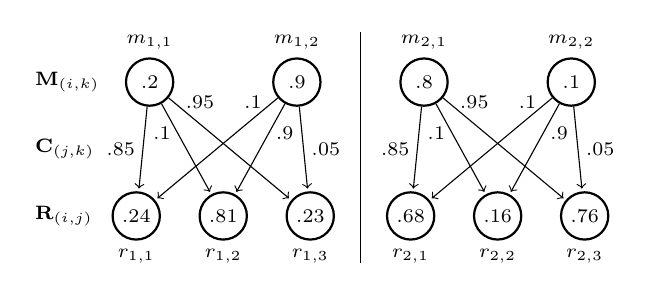
\begin{tikzpicture}[shorten >=1pt,->,draw=black!100, scale=0.85]
	\footnotesize
%	\def \attic{5.95cm}
%	\def \rowtwoht{5.4cm}
%	\def \weightlevel{3.9cm}
%	\def \rowoneht{2.4cm}
%	\def \basement{1.8cm}
%	\def \data{1cm}
%	\def \china{0cm}

	\def \attic{5cm}
	\def \rowtwoht{4.4cm}
	\def \weightlevel{3.4cm}
	\def \rowoneht{2.4cm}
	\def \basement{1.8cm}
	\def \data{1cm}
	\def \china{0cm}
		
	\tikzstyle{m-node}=[circle,draw=black!100,thick,inner sep=0pt,minimum size=6mm]
	\tikzstyle{r-node}=[circle,draw=black!100,thick,inner sep=0pt,minimum size=6mm]
	\tikzstyle{d-node}=[circle,draw=black!100,fill=gray!45,thick,inner sep=0pt,minimum size=6mm]
	%\tikzstyle{dots}=[text width=5ex, text centered]
	\tikzstyle{annot}=[text width=2.5em]
	% labels
	\tikzstyle{label}=[text width=2.5em, text centered]
	\tikzstyle{formula}=[text width=30em, text centered]
	
	\scriptsize
	\node[annot] (hidden-layer) at (0cm,\rowtwoht) {$\mathbf{M}_{(i,k)}$};
	\node[annot] (weights) at (0cm,\weightlevel) {$\mathbf{C}_{(j,k)}$};
	\node[annot] (r-layer) at (0cm,\rowoneht) {$\mathbf{R}_{(i,j)}$};
	
	% hidden layer
	\scriptsize
	\node[m-node] 	(ma00)	at (1.3cm,\rowtwoht)		{$.2$};
	\node[m-node] 	(ma01)	at (3.5cm,\rowtwoht)		{$.9$};
	\node[m-node] 	(ma10)	at (5.4cm,\rowtwoht) 	{$.8$};
	\node[m-node] 	(ma11)	at (7.6cm,\rowtwoht)	 	{$.1$};
	% \node[m-node] 	(m20)	at (9.65cm,\rowtwoht) 	{$.8$};
	% \node[m-node] 	(m21)	at (11.55cm,\rowtwoht)	 	{$.9$};
	
	%\footnotesize
	\node[label]	(ml00) 	at (1.3cm,\attic)		{$m_{1,1}$}; %1.75 -> 1.45
	\node[label]	(ml01) 	at (3.5cm,\attic)		{$m_{1,2}$}; %3.05 -> 3.35
	\node[label] 	(ml10)	at (5.4cm,\attic) 	{$m_{2,1}$};     %5.85 -> 5.55
	\node[label] 	(ml11)	at (7.6cm,\attic)	 	{$m_{2,2}$}; %7.15 -> 7.45
	% \node[label] 	(ml20)	at (9.65cm,\attic) 	{$m_{3,1}$};     %9.95 -> 9.65
	% \node[label] 	(ml21)	at (11.55cm,\attic)	 	{$m_{3,2}$}; %11.25 -> 11.55
	
	\scriptsize
	\node[r-node] 	(ra00)	at (1.1cm,\rowoneht)		{$.24$};
	\node[r-node] 	(ra01)	at (2.4cm,\rowoneht)		{$.81$};
	\node[r-node] 	(ra02)	at (3.7cm,\rowoneht)	 	{$.23$};
	
	\node[r-node] 	(ra10)	at (5.2cm,\rowoneht) 		{$.68$};
	\node[r-node] 	(ra11) 	at (6.5cm,\rowoneht)   	{$.16$};
	\node[r-node] 	(ra12)	at (7.8cm,\rowoneht)		{$.76$};
	
	% \node[r-node] 	(r20) 	at (9.3cm,\rowoneht)  		{$.71$};
	% \node[r-node] 	(r21)	at (10.6cm,\rowoneht) 		{$.83$};
	% \node[r-node] 	(r22) 	at (11.9cm,\rowoneht)   	{$.77$};
	
	\node[label] 	(rl00)	at (1.1cm,\basement)		{$r_{1,1}$};
	\node[label] 	(rl01)	at (2.4cm,\basement)		{$r_{1,2}$};
	\node[label] 	(rl02)	at (3.7cm,\basement)	 	{$r_{1,3}$};
	
	\node[label] 	(rl10)	at (5.2cm,\basement) 		{$r_{2,1}$};
	\node[label] 	(rl11) 	at (6.5cm,\basement)   	{$r_{2,2}$};
	\node[label] 	(rl12)	at (7.8cm,\basement)		{$r_{2,3}$};
	
%	\node[label] 	(rl20) 	at (9.3cm,\basement)  		{$r_{3,1}$};
%	\node[label] 	(rl21)	at (10.6cm,\basement) 		{$r_{3,2}$};
%	\node[label] 	(rl22) 	at (11.9cm,\basement)   	{$r_{3,3}$};

	\draw[-] (4.45cm, \attic+1.5mm) -- (4.45cm, \basement-1.5mm);
%	\draw[-] (8.55cm, \attic+1.5mm) -- (8.55cm, \basement-1.5mm);

	\scriptsize
	\path
		(ma00)	edge	node [left]	{$.85$} (ra00)
		(ma00)	edge	node [left,xshift=-1mm,yshift=2mm]	{$.1$}	(ra01)
		(ma00)	edge	node [left,xshift=-1mm,yshift=6mm]	{$.95$}	(ra02)

		(ma01)	edge	node [right,xshift=2.5mm,yshift=6mm]	{$.1$}	(ra00)
		(ma01)	edge	node [right,xshift=1mm,yshift=2mm]	{$.9$}	(ra01)
		(ma01)	edge	node [right]	{$.05$} (ra02)
		%
		(ma10)	edge	node [left] {$.85$} (ra10)
		(ma10)	edge	node [left,xshift=-1mm,yshift=2mm]	{$.1$}	(ra11)
		(ma10)	edge	node [left,xshift=-1mm,yshift=6mm] {$.95$}	(ra12)
		
		(ma11)	edge	node [right,xshift=2.5mm,yshift=6mm]	{$.1$}	(ra10)
		(ma11)	edge	node [right,xshift=1mm,yshift=2mm]	{$.9$}	(ra11)
		(ma11)	edge	node [right]	{$.05$} (ra12);
		%
		% (m20)	edge	node [left]	{$.85$}	(r20)
		% (m20)	edge	node [left,xshift=-1mm,yshift=4mm]	{$.1$}	(r21)
		% (m20)	edge	node [left,xshift=-1mm,yshift=10mm]	{$.95$} (r22)
		
		% (m21)	edge	node [right,xshift=3mm,yshift=10mm]		{$.1$}	(r20)
		% (m21)	edge	node [right,xshift=1mm,yshift=4mm]{$.9$}	(r21)
		% (m21)	edge	node [right]	{$.05$}	(r22);		
		
\end{tikzpicture}
\label{fig:example:subfig1}
}
\subfigure[Convergence]{

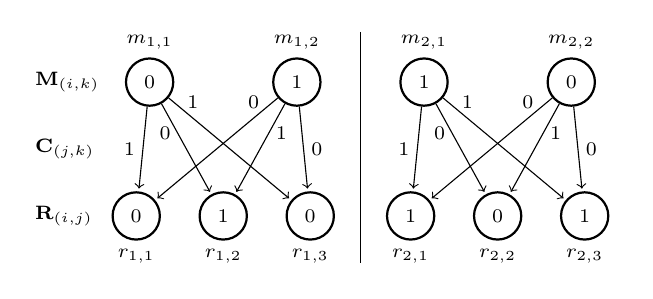
\begin{tikzpicture}[shorten >=1pt,->,draw=black!100, scale=0.85]
	\footnotesize
%	\def \attic{5.95cm}
%	\def \rowtwoht{5.4cm}
%	\def \weightlevel{3.9cm}
%	\def \rowoneht{2.4cm}
%	\def \basement{1.8cm}
%	\def \data{1cm}
%	\def \china{0cm}

%	\def \attic{5.2cm}
%	\def \rowtwoht{4.6cm}
%	\def \weightlevel{3.5cm}
%	\def \rowoneht{2.4cm}
%	\def \basement{1.8cm}
%	\def \data{1cm}
%	\def \china{0cm}

	\def \attic{5cm}
	\def \rowtwoht{4.4cm}
	\def \weightlevel{3.4cm}
	\def \rowoneht{2.4cm}
	\def \basement{1.8cm}
	\def \data{1cm}
	\def \china{0cm}
		
%	\def \attic{5.4cm}
%	\def \rowtwoht{5cm}
%	\def \weightlevel{3.9cm}
%	\def \rowoneht{2.4cm}
%	\def \basement{1.8cm}
%	\def \data{1cm}
%	\def \china{0cm}
	
	\scriptsize
	\tikzstyle{m-node}=[circle,draw=black!100,thick,inner sep=0pt,minimum size=6mm]
	\tikzstyle{r-node}=[circle,draw=black!100,thick,inner sep=0pt,minimum size=6mm]
	\tikzstyle{d-node}=[circle,draw=black!100,fill=gray!45,thick,inner sep=0pt,minimum size=6mm]
	\tikzstyle{annot}=[text width=2.5em]
	% labels
	\tikzstyle{label}=[text width=3em, text centered]
	\tikzstyle{formula}=[text width=30em, text centered]
	\node[annot] (hidden-layer) at (0cm,\rowtwoht) {$\mathbf{M}_{(i,k)}$};
	\node[annot] (weights) at (0cm,\weightlevel) {$\mathbf{C}_{(j,k)}$};
	\node[annot] (r-layer) at (0cm,\rowoneht) {$\mathbf{R}_{(i,j)}$};
	
	\node[m-node] 	(m00)	at (1.3cm,\rowtwoht)		{$0$};
	\node[m-node] 	(m01)	at (3.5cm,\rowtwoht)		{$1$};
	\node[m-node] 	(m10)	at (5.4cm,\rowtwoht) 	{$1$};
	\node[m-node] 	(m11)	at (7.6cm,\rowtwoht)	 	{$0$};
	% \node[m-node] 	(m20)	at (9.65cm,\rowtwoht) 	{$1$};
	% \node[m-node] 	(m21)	at (11.55cm,\rowtwoht)	 	{$1$};
	
	\node[label]	(ml00) 	at (1.3cm,\attic)		{$m_{1,1}$};
	\node[label]	(ml01) 	at (3.5cm,\attic)		{$m_{1,2}$};
	\node[label] 	(ml10)	at (5.4cm,\attic) 	{$m_{2,1}$};
	\node[label] 	(ml11)	at (7.6cm,\attic)	 	{$m_{2,2}$};
	% \node[label] 	(ml20)	at (9.65cm,\attic) 	{$m_{3,1}$};
	% \node[label] 	(ml21)	at (11.55cm,\attic)	 	{$m_{3,2}$};
	
	%\node[m-node] 	(m20)	[right of=m11,xshift=2cm]	 	{$1.0$};
	%\node[m-node] 	(m21)	[right of=m20,xshift=0.5cm]	 	{$1.0$};	
	% reconstructed vector
	\node[r-node] 	(r00)	at (1.1cm,\rowoneht)		{$0$};
	\node[label] 	(rl00)	at (1.1cm,\basement)		{$r_{1,1}$};
	\node[r-node] 	(r01)	at (2.4cm,\rowoneht)		{$1$};
	\node[label] 	(rl01)	at (2.4cm,\basement)		{$r_{1,2}$};
	\node[r-node] 	(r02)	at (3.7cm,\rowoneht)	 	{$0$};
	\node[label] 	(rl02)	at (3.7cm,\basement)	 	{$r_{1,3}$};
	
	\node[r-node] 	(r10)	at (5.2cm,\rowoneht) 		{$1$};
	\node[label] 	(rl10)	at (5.2cm,\basement) 		{$r_{2,1}$};
	\node[r-node] 	(r11) 	at (6.5cm,\rowoneht)   		{$0$};
	\node[label] 	(rl11) 	at (6.5cm,\basement)   		{$r_{2,2}$};
	\node[r-node] 	(r12)	at (7.8cm,\rowoneht)		{$1$};
	\node[label] 	(rl12)	at (7.8cm,\basement)		{$r_{2,3}$};
	
	% \node[r-node] 	(r20) 	at (9.3cm,\rowoneht)  		{$1$};
	% \node[label] 	(rl20) 	at (9.3cm,\basement)  		{$r_{3,1}$};
	% \node[r-node] 	(r21)	at (10.6cm,\rowoneht) 		{$1$};
	% \node[label] 	(rl21)	at (10.6cm,\basement) 		{$r_{3,2}$};
	% \node[r-node] 	(r22) 	at (11.9cm,\rowoneht)   		{$1$};
	% \node[label] 	(rl22) 	at (11.9cm,\basement)   		{$r_{3,3}$};
	
	\draw[-] (4.45cm, \attic+1.5mm) -- (4.45cm, \basement-1.5mm);
%	\draw[-] (8.55cm, \attic+1.5mm) -- (8.55cm, \basement-1.5mm);

	\path
		(m00)	edge	node [left] 	{$1$}	(r00)
		(m00)	edge	node [left,xshift=-1mm,yshift=2mm]	{$0$}	(r01)
		(m00)	edge	node [left,xshift=-3mm,yshift=6mm]	{$1$}	(r02)

		(m01)	edge	node [right,xshift=3mm,yshift=6mm]	{$0$}	(r00)
		(m01)	edge	node [right,xshift=1mm,yshift=2mm]	{$1$}	(r01)
		(m01)	edge	node [right]	{$0$}	(r02)
		%
		(m10)	edge	node [left] 	{$1$}	(r10)
		(m10)	edge	node [left,xshift=-1mm,yshift=2mm]	{$0$}	(r11)
		(m10)	edge	node [left,xshift=-3mm,yshift=6mm] {$1$}	(r12)
		
		(m11)	edge	node [right,xshift=3mm,yshift=6mm]	{$0$}	(r10)
		(m11)	edge	node [right,xshift=1mm,yshift=2mm]	{$1$}	(r11)
		(m11)	edge	node [right]	{$0$}	(r12);
		%
		% (m20)	edge	node [left]	{$1$}	(r20)
		% (m20)	edge	node [left,xshift=-1mm,yshift=4mm]	{$0$}	(r21)
		% (m20)	edge	node [left,xshift=-3mm,yshift=10mm]	{$1$} (r22)
		
		% (m21)	edge	node [right,xshift=3mm,yshift=10mm]		{$0$}	(r20)
		% (m21)	edge	node [right,xshift=1mm,yshift=4mm]{$1$}	(r21)
		% (m21)	edge	node [right]	{$0$}	(r22);		
\end{tikzpicture}
\label{fig:example:subfig2}
}

\begin{framed}
	\centering
	\small
	where
	$\begin{aligned}
	   r_{i,j} = 1 - \Pi_{k=1}^{K} (1 - m_{i,k}c_{j,k}) 
	\end{aligned}$
        \hspace{2em}
        [\textsc{noisy-or} function]
\end{framed}

\end{center}
\caption{A simple MCMM example} % showing learning in progress}
\label{fig:example}
\end{figure}

We can see that while learning is in progress, the cluster activities
($m_{i,k}$) and the cluster centers ($c_{j,k}$) are in flux, as the
error rate is being reduced, but that they converge to values of 0 and
1.  At convergence, a reconstruction node ($r_{i,j}$) is 1 if at least one
$m_{i,k}c_{j,k} = 1$ (and 0 otherwise).

%the activities and the centers are 1 and are 0 otherwise.

% \begin{figure*}[htb]
% \usetikzlibrary{positioning}
% \begin{center}
% \subfigure[Observed Data]{
% \begin{tikzpicture}[shorten >=1pt,->,draw=black!100]
% 	\scriptsize
% 	\tikzstyle{label}=[text width=3em, text centered]
% 	\tikzstyle{annot}=[text width=2.5em]
% 	\tikzstyle{d-node}=[circle,draw=black!100,fill=gray!45,thick,inner sep=0pt,minimum size=6mm]
	
% 	\def \china{0.6cm}
% 	\def \data{0cm}
	
% 	\node[annot] (d-layer) at (0cm,\data) {$\mathbf{D}_{(i,j)}$};
% 	\draw[-] (4.45cm, \china+1.5mm) -- (4.45cm, \data-4.5mm);
% 	\draw[-] (8.55cm, \china+1.5mm) -- (8.55cm, \data-4.5mm);
% 	%\draw[-] (-1cm, \china+.5cm) -- (13cm, \china+.5cm);
% 	%\draw[-] (-1cm, \data-.5cm) -- (13cm, \data-.5cm);
	
% 	\node[label] 	(dl00)	at (1.1cm,\china)		{$d_{1,1}$};
% 	\node[label] 	(dl01)	at (2.4cm,\china)		{$d_{1,2}$};
% 	\node[label] 	(dl02)	at (3.7cm,\china)	 	{$d_{1,3}$};
	
% 	\node[label] 	(dl10)	at (5.2cm,\china) 		{$d_{2,1}$};
% 	\node[label] 	(dl11) 	at (6.5cm,\china)   	{$d_{2,2}$};
% 	\node[label] 	(dl12)	at (7.8cm,\china)		{$d_{2,3}$};
	
% 	\node[label] 	(dl20) 	at (9.3cm,\china)  		{$d_{3,1}$};
% 	\node[label] 	(dl21)	at (10.6cm,\china) 		{$d_{3,2}$};
% 	\node[label] 	(dl22) 	at (11.9cm,\china)   	{$d_{3,3}$};
	
% 	\node[d-node] 	(d00)	at (1.1cm,\data)		{$0$};
% 	\node[d-node] 	(d01)	at (2.4cm,\data)		{$1$};
% 	\node[d-node] 	(d02)	at (3.7cm,\data)		{$0$};

% 	\node[d-node] 	(d10)	at (5.2cm,\data)		{$1$};
% 	\node[d-node] 	(d11)	at (6.5cm,\data)		{$0$};
% 	\node[d-node] 	(d12)	at (7.8cm,\data)		{$1$};
	
% 	\node[d-node] 	(d20)	at (9.3cm,\data)		{$1$};
% 	\node[d-node] 	(d21)	at (10.6cm,\data)		{$1$};
% 	\node[d-node] 	(d22)	at (11.9cm,\data)		{$1$};
% \end{tikzpicture}
% \label{fig:example:subfig0}
% }
% \end{center}

% \usetikzlibrary{positioning}
% %\begin{minipage}{.3\textwidth}
% \begin{center}
% \subfigure[Learning in Progress]{
% \begin{tikzpicture}[shorten >=1pt,->,draw=black!100]
% 	\footnotesize
% 	\def \attic{5.95cm}
% 	\def \rowtwoht{5.4cm}
% 	\def \weightlevel{3.9cm}
% 	\def \rowoneht{2.4cm}
% 	\def \basement{1.8cm}
% 	\def \data{1cm}
% 	\def \china{0cm}
	
% 	\tikzstyle{m-node}=[circle,draw=black!100,thick,inner sep=0pt,minimum size=6mm]
% 	\tikzstyle{r-node}=[circle,draw=black!100,thick,inner sep=0pt,minimum size=6mm]
% 	\tikzstyle{d-node}=[circle,draw=black!100,fill=gray!45,thick,inner sep=0pt,minimum size=6mm]
% 	%\tikzstyle{dots}=[text width=5ex, text centered]
% 	\tikzstyle{annot}=[text width=2.5em]
% 	% labels
% 	\tikzstyle{label}=[text width=3em, text centered]
% 	\tikzstyle{formula}=[text width=30em, text centered]
	
% 	\scriptsize
% 	\node[annot] (hidden-layer) at (0cm,\rowtwoht) {$\mathbf{M}_{(i,k)}$};
% 	\node[annot] (weights) at (0cm,\weightlevel) {$\mathbf{C}_{(j,k)}$};
% 	\node[annot] (r-layer) at (0cm,\rowoneht) {$\mathbf{R}_{(i,j)}$};
	
% 	% hidden layer
% 	\scriptsize
% 	\node[m-node] 	(m00)	at (1.45cm,\rowtwoht)		{$.2$};
% 	\node[m-node] 	(m01)	at (3.35cm,\rowtwoht)		{$.9$};
% 	\node[m-node] 	(m10)	at (5.55cm,\rowtwoht) 	{$.8$};
% 	\node[m-node] 	(m11)	at (7.45cm,\rowtwoht)	 	{$.1$};
% 	\node[m-node] 	(m20)	at (9.65cm,\rowtwoht) 	{$.8$};
% 	\node[m-node] 	(m21)	at (11.55cm,\rowtwoht)	 	{$.9$};
	
% 	%\footnotesize
% 	\node[label]	(ml00) 	at (1.45cm,\attic)		{$m_{1,1}$}; %1.75 -> 1.45
% 	\node[label]	(ml01) 	at (3.35cm,\attic)		{$m_{1,2}$}; %3.05 -> 3.35
% 	\node[label] 	(ml10)	at (5.55cm,\attic) 	{$m_{2,1}$};     %5.85 -> 5.55
% 	\node[label] 	(ml11)	at (7.45cm,\attic)	 	{$m_{2,2}$}; %7.15 -> 7.45
% 	\node[label] 	(ml20)	at (9.65cm,\attic) 	{$m_{3,1}$};     %9.95 -> 9.65
% 	\node[label] 	(ml21)	at (11.55cm,\attic)	 	{$m_{3,2}$}; %11.25 -> 11.55
	
% 	\scriptsize
% 	\node[r-node] 	(r00)	at (1.1cm,\rowoneht)		{$.24$};
% 	\node[r-node] 	(r01)	at (2.4cm,\rowoneht)		{$.81$};
% 	\node[r-node] 	(r02)	at (3.7cm,\rowoneht)	 	{$.23$};
	
% 	\node[r-node] 	(r10)	at (5.2cm,\rowoneht) 		{$.68$};
% 	\node[r-node] 	(r11) 	at (6.5cm,\rowoneht)   	{$.16$};
% 	\node[r-node] 	(r12)	at (7.8cm,\rowoneht)		{$.76$};
	
% 	\node[r-node] 	(r20) 	at (9.3cm,\rowoneht)  		{$.71$};
% 	\node[r-node] 	(r21)	at (10.6cm,\rowoneht) 		{$.83$};
% 	\node[r-node] 	(r22) 	at (11.9cm,\rowoneht)   	{$.77$};
	
% 	\node[label] 	(rl00)	at (1.1cm,\basement)		{$r_{1,1}$};
% 	\node[label] 	(rl01)	at (2.4cm,\basement)		{$r_{1,2}$};
% 	\node[label] 	(rl02)	at (3.7cm,\basement)	 	{$r_{1,3}$};
	
% 	\node[label] 	(rl10)	at (5.2cm,\basement) 		{$r_{2,1}$};
% 	\node[label] 	(rl11) 	at (6.5cm,\basement)   	{$r_{2,2}$};
% 	\node[label] 	(rl12)	at (7.8cm,\basement)		{$r_{2,3}$};
	
% 	\node[label] 	(rl20) 	at (9.3cm,\basement)  		{$r_{3,1}$};
% 	\node[label] 	(rl21)	at (10.6cm,\basement) 		{$r_{3,2}$};
% 	\node[label] 	(rl22) 	at (11.9cm,\basement)   	{$r_{3,3}$};

% 	\draw[-] (4.45cm, \attic+1.5mm) -- (4.45cm, \basement-1.5mm);
% 	\draw[-] (8.55cm, \attic+1.5mm) -- (8.55cm, \basement-1.5mm);

% 	\scriptsize
% 	\path
% 		(m00)	edge	node [left] 	{$.85$}	(r00)
% 		(m00)	edge	node [left,xshift=-1mm,yshift=4mm]	{$.1$}	(r01)
% 		(m00)	edge	node [left,xshift=-1mm,yshift=10mm]	{$.95$}	(r02)

% 		(m01)	edge	node [right,xshift=3mm,yshift=10mm]	{$.1$}	(r00)
% 		(m01)	edge	node [right,xshift=1mm,yshift=4mm]	{$.9$}	(r01)
% 		(m01)	edge	node [right]	{$.05$}	(r02)
% 		%
% 		(m10)	edge	node [left] 	{$.85$}	(r10)
% 		(m10)	edge	node [left,xshift=-1mm,yshift=4mm]	{$.1$}	(r11)
% 		(m10)	edge	node [left,xshift=-1mm,yshift=10mm] {$.95$}	(r12)
		
% 		(m11)	edge	node [right,xshift=3mm,yshift=10mm]	{$.1$}	(r10)
% 		(m11)	edge	node [right,xshift=1mm,yshift=4mm]	{$.9$}	(r11)
% 		(m11)	edge	node [right]	{$.05$}	(r12)
% 		%
% 		(m20)	edge	node [left]	{$.85$}	(r20)
% 		(m20)	edge	node [left,xshift=-1mm,yshift=4mm]	{$.1$}	(r21)
% 		(m20)	edge	node [left,xshift=-1mm,yshift=10mm]	{$.95$} (r22)
		
% 		(m21)	edge	node [right,xshift=3mm,yshift=10mm]		{$.1$}	(r20)
% 		(m21)	edge	node [right,xshift=1mm,yshift=4mm]{$.9$}	(r21)
% 		(m21)	edge	node [right]	{$.05$}	(r22);		
		
% \end{tikzpicture}
% \label{fig:example:subfig1}
% }
% \subfigure[Convergence]{

% \begin{tikzpicture}[shorten >=1pt,->,draw=black!100]
% 	\footnotesize
% 	\def \attic{5.95cm}
% 	\def \rowtwoht{5.4cm}
% 	\def \weightlevel{3.9cm}
% 	\def \rowoneht{2.4cm}
% 	\def \basement{1.8cm}
% 	\def \data{1cm}
% 	\def \china{0cm}
	
% 	\scriptsize
% 	\tikzstyle{m-node}=[circle,draw=black!100,thick,inner sep=0pt,minimum size=6mm]
% 	\tikzstyle{r-node}=[circle,draw=black!100,thick,inner sep=0pt,minimum size=6mm]
% 	\tikzstyle{d-node}=[circle,draw=black!100,fill=gray!45,thick,inner sep=0pt,minimum size=6mm]
% 	\tikzstyle{annot}=[text width=2.5em]
% 	% labels
% 	\tikzstyle{label}=[text width=3em, text centered]
% 	\tikzstyle{formula}=[text width=30em, text centered]
% 	\node[annot] (hidden-layer) at (0cm,\rowtwoht) {$\mathbf{M}_{(i,k)}$};
% 	\node[annot] (weights) at (0cm,\weightlevel) {$\mathbf{C}_{(j,k)}$};
% 	\node[annot] (r-layer) at (0cm,\rowoneht) {$\mathbf{R}_{(i,j)}$};
	
% 	\node[m-node] 	(m00)	at (1.45cm,\rowtwoht)		{$0$};
% 	\node[m-node] 	(m01)	at (3.35cm,\rowtwoht)		{$1$};
% 	\node[m-node] 	(m10)	at (5.55cm,\rowtwoht) 	{$1$};
% 	\node[m-node] 	(m11)	at (7.45cm,\rowtwoht)	 	{$0$};
% 	\node[m-node] 	(m20)	at (9.65cm,\rowtwoht) 	{$1$};
% 	\node[m-node] 	(m21)	at (11.55cm,\rowtwoht)	 	{$1$};
	
% 	\node[label]	(ml00) 	at (1.45cm,\attic)		{$m_{1,1}$};
% 	\node[label]	(ml01) 	at (3.35cm,\attic)		{$m_{1,2}$};
% 	\node[label] 	(ml10)	at (5.55cm,\attic) 	{$m_{2,1}$};
% 	\node[label] 	(ml11)	at (7.45cm,\attic)	 	{$m_{2,2}$};
% 	\node[label] 	(ml20)	at (9.65cm,\attic) 	{$m_{3,1}$};
% 	\node[label] 	(ml21)	at (11.55cm,\attic)	 	{$m_{3,2}$};
	
% 	%\node[m-node] 	(m20)	[right of=m11,xshift=2cm]	 	{$1.0$};
% 	%\node[m-node] 	(m21)	[right of=m20,xshift=0.5cm]	 	{$1.0$};	
% 	% reconstructed vector
% 	\node[r-node] 	(r00)	at (1.1cm,\rowoneht)		{$0$};
% 	\node[label] 	(rl00)	at (1.1cm,\basement)		{$r_{1,1}$};
% 	\node[r-node] 	(r01)	at (2.4cm,\rowoneht)		{$1$};
% 	\node[label] 	(rl01)	at (2.4cm,\basement)		{$r_{1,2}$};
% 	\node[r-node] 	(r02)	at (3.7cm,\rowoneht)	 	{$0$};
% 	\node[label] 	(rl02)	at (3.7cm,\basement)	 	{$r_{1,3}$};
	
% 	\node[r-node] 	(r10)	at (5.2cm,\rowoneht) 		{$1$};
% 	\node[label] 	(rl10)	at (5.2cm,\basement) 		{$r_{2,1}$};
% 	\node[r-node] 	(r11) 	at (6.5cm,\rowoneht)   		{$0$};
% 	\node[label] 	(rl11) 	at (6.5cm,\basement)   		{$r_{2,2}$};
% 	\node[r-node] 	(r12)	at (7.8cm,\rowoneht)		{$1$};
% 	\node[label] 	(rl12)	at (7.8cm,\basement)		{$r_{2,3}$};
	
% 	\node[r-node] 	(r20) 	at (9.3cm,\rowoneht)  		{$1$};
% 	\node[label] 	(rl20) 	at (9.3cm,\basement)  		{$r_{3,1}$};
% 	\node[r-node] 	(r21)	at (10.6cm,\rowoneht) 		{$1$};
% 	\node[label] 	(rl21)	at (10.6cm,\basement) 		{$r_{3,2}$};
% 	\node[r-node] 	(r22) 	at (11.9cm,\rowoneht)   		{$1$};
% 	\node[label] 	(rl22) 	at (11.9cm,\basement)   		{$r_{3,3}$};
	
% 	\draw[-] (4.45cm, \attic+1.5mm) -- (4.45cm, \basement-1.5mm);
% 	\draw[-] (8.55cm, \attic+1.5mm) -- (8.55cm, \basement-1.5mm);

% 	\path
% 		(m00)	edge	node [left] 	{$1$}	(r00)
% 		(m00)	edge	node [left,xshift=-1mm,yshift=4mm]	{$0$}	(r01)
% 		(m00)	edge	node [left,xshift=-3mm,yshift=10mm]	{$1$}	(r02)

% 		(m01)	edge	node [right,xshift=3mm,yshift=10mm]	{$0$}	(r00)
% 		(m01)	edge	node [right,xshift=1mm,yshift=4mm]	{$1$}	(r01)
% 		(m01)	edge	node [right]	{$0$}	(r02)
% 		%
% 		(m10)	edge	node [left] 	{$1$}	(r10)
% 		(m10)	edge	node [left,xshift=-1mm,yshift=4mm]	{$0$}	(r11)
% 		(m10)	edge	node [left,xshift=-3mm,yshift=10mm] {$1$}	(r12)
		
% 		(m11)	edge	node [right,xshift=3mm,yshift=10mm]	{$0$}	(r10)
% 		(m11)	edge	node [right,xshift=1mm,yshift=4mm]	{$1$}	(r11)
% 		(m11)	edge	node [right]	{$0$}	(r12)
% 		%
% 		(m20)	edge	node [left]	{$1$}	(r20)
% 		(m20)	edge	node [left,xshift=-1mm,yshift=4mm]	{$0$}	(r21)
% 		(m20)	edge	node [left,xshift=-3mm,yshift=10mm]	{$1$} (r22)
		
% 		(m21)	edge	node [right,xshift=3mm,yshift=10mm]		{$0$}	(r20)
% 		(m21)	edge	node [right,xshift=1mm,yshift=4mm]{$1$}	(r21)
% 		(m21)	edge	node [right]	{$0$}	(r22);		
% \end{tikzpicture}
% \label{fig:example:subfig2}
% }

% \begin{framed}
% 	\centering
% 	\small
% 	where
% 	$\begin{aligned}
% 	   r_{i,j} = 1 - \Pi_{k=1}^{K} (1 - m_{i,k}c_{j,k}) 
% 	\end{aligned}$
% \end{framed}

% \label{fig:example}
% \caption{MCMM example showing learning in progress}
% \end{center}
% \end{figure*}

\subsection{MCMMs for Morphology}
\label{subsec:mcmm-morph}

% \marginpar{MD: I reduced the size of fig.~\ref{fig:morphexample},
%   requiring some fudging with the placement of weights}

\begin{figure*}[htb]
\begin{center}
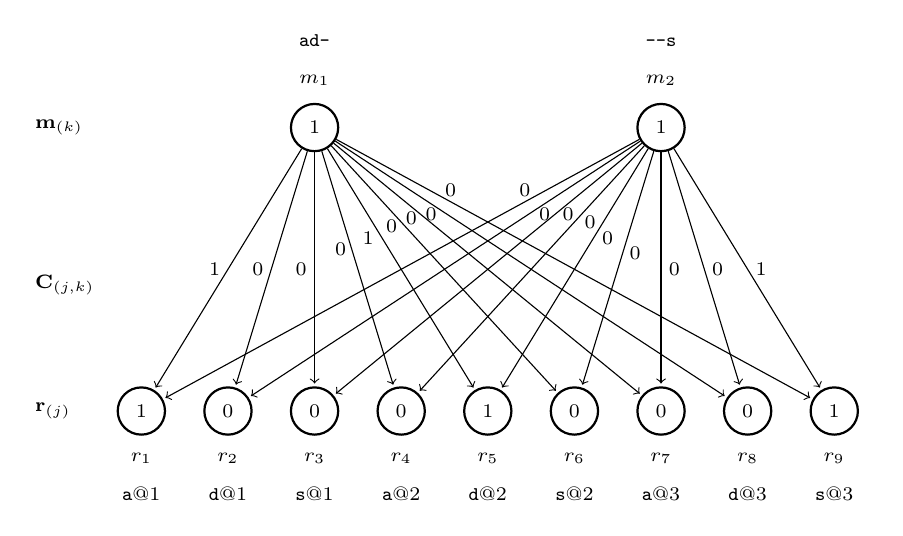
\begin{tikzpicture}[shorten >=1pt,->,draw=black!100]
	\footnotesize
	\def \roof{7.1cm}
	\def \attic{6.6cm}
	\def \rowtwoht{6cm}
	\def \weightlevel{4cm}
	\def \rowoneht{2.4cm}
	\def \basement{1.8cm}
	\def \data{1.35cm}
	\def \china{0cm}
	\def \shangrila{-0.6cm}
	
	\scriptsize
	\tikzstyle{m-node}=[circle,draw=black!100,thick,inner sep=0pt,minimum size=6mm]
	\tikzstyle{r-node}=[circle,draw=black!100,thick,inner sep=0pt,minimum size=6mm]
	\tikzstyle{d-node}=[circle,draw=black!100,fill=gray!45,thick,inner sep=0pt,minimum size=6mm]
	%\tikzstyle{dots}=[text width=5ex, text centered]
	\tikzstyle{annot}=[text width=2.5em]
	% labels
	\tikzstyle{label}=[text width=3em, text centered]
	\tikzstyle{formula}=[text width=30em, text centered]
	\node[annot] (hidden-layer) at (0cm,\rowtwoht) {$\mathbf{m}_{(k)}$};
	%\node[annot] (weights) at (0cm,\weightlevel) {weights ($\mathbf{M}$)};
	\node[annot] (weights) at (0cm,\weightlevel) {$\mathbf{C}_{(j,k)}$};
	%\node[annot] (d-layer) at (0cm,\data) {$\mathbf{D}_{(i,j)}$};
	\node[annot] (r-layer) at (0cm,\rowoneht) {$\mathbf{r}_{(j)}$}; %\mathbf{R}_{(i,j)
	
	\node[m-node] 	(m00)	at (3.2cm,\rowtwoht)		{$1$};
	\node[m-node] 	(m01)	at (7.6cm,\rowtwoht)		{$1$};
	
	\node[label]	(ml00) 	at (3.2cm,\attic)		{$m_{1}$};
	\node[label]	(ml01) 	at (7.6cm,\attic)		{$m_{2}$};
	
	\node[label]	(t1)	at (3.2cm,\roof)		{\texttt{ad-}};
	\node[label]	(t2)	at (7.6cm,\roof)		{\texttt{--s}};
		
	% reconstructed vector
	\node[r-node] 	(r00)	at (1.0cm,\rowoneht)		{$1$};
	\node[label] 	(rl00)	at (1.0cm,\basement)		{$r_{1}$};
	\node[label]	(b1)	at (1.0cm,\data)		{\texttt{a}@1};
	\node[r-node] 	(r01)	at (2.1cm,\rowoneht)		{$0$};
	\node[label] 	(rl01)	at (2.1cm,\basement)		{$r_{2}$};
	\node[label]	(b2)	at (2.1cm,\data)		{\texttt{d}@1};
	\node[r-node] 	(r02)	at (3.2cm,\rowoneht)	 	{$0$};
	\node[label] 	(rl02)	at (3.2cm,\basement)	 	{$r_{3}$};
	\node[label]	(b3)	at (3.2cm,\data)		{\texttt{s}@1};
	
	\node[r-node] 	(r03)	at (4.3cm,\rowoneht)	 	{$0$};
	\node[label] 	(rl03)	at (4.3cm,\basement)	 	{$r_{4}$};
	\node[label]	(b4)	at (4.3cm, \data)		{\texttt{a}@2};
	\node[r-node] 	(r04)	at (5.4cm,\rowoneht)	 	{$1$};
	\node[label] 	(rl04)	at (5.4cm,\basement)	 	{$r_{5}$};
	\node[label]	(b5)	at (5.4cm, \data)		{\texttt{d}@2};
	\node[r-node] 	(r05)	at (6.5cm,\rowoneht)	 	{$0$};
	\node[label] 	(rl05)	at (6.5cm,\basement)	 	{$r_{6}$};
	\node[label]	(b6)	at (6.5cm, \data)		{\texttt{s}@2};
	
	\node[r-node] 	(r06)	at (7.6cm,\rowoneht)	 	{$0$};
	\node[label] 	(rl06)	at (7.6cm,\basement)	 	{$r_{7}$};
	\node[label]	(b4)	at (7.6cm, \data)		{\texttt{a}@3};
	\node[r-node] 	(r07)	at (8.7cm,\rowoneht)	 	{$0$};
	\node[label] 	(rl07)	at (8.7cm,\basement)	 	{$r_{8}$};
	\node[label]	(b5)	at (8.7cm, \data)		{\texttt{d}@3};
	\node[r-node] 	(r08)	at (9.8cm,\rowoneht)	 	{$1$};
	\node[label] 	(rl08)	at (9.8cm,\basement)	 	{$r_{9}$};
	\node[label]	(b6)	at (9.8cm, \data)		{\texttt{s}@3};
	
%	\node[formula] (r-formula) at (6.1cm,\china)
%	   {\small where {
%	   $\begin{aligned}
%	   r_{i,j} = 1 - \big( 1 - \Pi_{k=1}^{K} (1 - m_{i,k}c_{j,k}) \big)
%	   \end{aligned}$}};
	
%	\draw[-] (4.45cm, \attic+1.5mm) -- (4.45cm, \basement-1.5mm);
%	\draw[-] (8.55cm, \attic+1.5mm) -- (8.55cm, \basement-1.5mm);

	\path
		(m00)	edge	node [left,xshift=0mm,yshift=0mm] 	{$1$}	(r00)
		(m00)	edge	node [left,xshift=-0mm,yshift=0.0mm] 	{$0$}	(r01)
		(m00)	edge	node [left,xshift=-0mm,yshift=0.0mm] 	{$0$}	(r02)
		(m00)	edge	node [left,xshift=-0.5mm,yshift=2.5mm] 	{$0$}	(r03)
		(m00)	edge	node [left,xshift=-2.5mm,yshift=4mm] 	{$1$}	(r04)
		(m00)	edge	node [left,xshift=-5mm,yshift=5.5mm] 	{$0$}	(r05)
		(m00)	edge	node [left,xshift=-8mm,yshift=6.5mm] 	{$0$}	(r06)
		(m00)	edge	node [left,xshift=-11mm,yshift=7mm] 	{$0$}	(r07)
		(m00)	edge	node [left,xshift=-14mm,yshift=10mm] 	{$0$}	(r08)

		(m01)	edge	node [right,xshift=14mm,yshift=10mm] 	{$0$}	(r00)
		(m01)	edge	node [right,xshift=11mm,yshift=7mm] 	{$0$}	(r01)
		(m01)	edge	node [right,xshift=8.5mm,yshift=7.0mm] 	{$0$}	(r02)
		(m01)	edge	node [right,xshift=5.8mm,yshift=6.0mm] 	{$0$}	(r03)
		(m01)	edge	node [right,xshift=2.5mm,yshift=4mm] 	{$0$}	(r04)
		(m01)	edge	node [right,xshift=0.5mm,yshift=2mm] 	{$0$}	(r05)
		(m01)	edge	node [right,xshift=0mm,yshift=0mm] 	{$0$}	(r06)
		(m01)	edge	node [right,xshift=0mm,yshift=0mm] 	{$0$}	(r07)
		(m01)	edge	node [right,xshift=0mm,yshift=0mm] 	{$1$}	(r08);		
\end{tikzpicture}

% \begin{tikzpicture}[shorten >=1pt,->,draw=black!100]
% 	\footnotesize
% 	\def \roof{8.5cm}
% 	\def \attic{8cm}
% 	\def \rowtwoht{7.4cm}
% 	\def \weightlevel{4.9cm}
% 	\def \rowoneht{2.4cm}
% 	\def \basement{1.8cm}
% 	\def \data{1.35cm}
% 	\def \china{0cm}
% 	\def \shangrila{-0.6cm}
	
% 	\scriptsize
% 	\tikzstyle{m-node}=[circle,draw=black!100,thick,inner sep=0pt,minimum size=6mm]
% 	\tikzstyle{r-node}=[circle,draw=black!100,thick,inner sep=0pt,minimum size=6mm]
% 	\tikzstyle{d-node}=[circle,draw=black!100,fill=gray!45,thick,inner sep=0pt,minimum size=6mm]
% 	%\tikzstyle{dots}=[text width=5ex, text centered]
% 	\tikzstyle{annot}=[text width=2.5em]
% 	% labels
% 	\tikzstyle{label}=[text width=3em, text centered]
% 	\tikzstyle{formula}=[text width=30em, text centered]
% 	\node[annot] (hidden-layer) at (0cm,\rowtwoht) {$\mathbf{m}_{(k)}$};
% 	%\node[annot] (weights) at (0cm,\weightlevel) {weights ($\mathbf{M}$)};
% 	\node[annot] (weights) at (0cm,\weightlevel) {$\mathbf{C}_{(j,k)}$};
% 	%\node[annot] (d-layer) at (0cm,\data) {$\mathbf{D}_{(i,j)}$};
% 	\node[annot] (r-layer) at (0cm,\rowoneht) {$\mathbf{r}_{(j)}$}; %\mathbf{R}_{(i,j)
	
% 	\node[m-node] 	(m00)	at (3.2cm,\rowtwoht)		{$1$};
% 	\node[m-node] 	(m01)	at (7.6cm,\rowtwoht)		{$1$};
	
% 	\node[label]	(ml00) 	at (3.2cm,\attic)		{$m_{1}$};
% 	\node[label]	(ml01) 	at (7.6cm,\attic)		{$m_{2}$};
	
% 	\node[label]	(t1)	at (3.2cm,\roof)		{\texttt{ad-}};
% 	\node[label]	(t2)	at (7.6cm,\roof)		{\texttt{--s}};
		
% 	% reconstructed vector
% 	\node[r-node] 	(r00)	at (1.0cm,\rowoneht)		{$1$};
% 	\node[label] 	(rl00)	at (1.0cm,\basement)		{$r_{1}$};
% 	\node[label]	(b1)	at (1.0cm,\data)		{\texttt{a}@1};
% 	\node[r-node] 	(r01)	at (2.1cm,\rowoneht)		{$0$};
% 	\node[label] 	(rl01)	at (2.1cm,\basement)		{$r_{2}$};
% 	\node[label]	(b2)	at (2.1cm,\data)		{\texttt{d}@1};
% 	\node[r-node] 	(r02)	at (3.2cm,\rowoneht)	 	{$0$};
% 	\node[label] 	(rl02)	at (3.2cm,\basement)	 	{$r_{3}$};
% 	\node[label]	(b3)	at (3.2cm,\data)		{\texttt{s}@1};
	
% 	\node[r-node] 	(r03)	at (4.3cm,\rowoneht)	 	{$0$};
% 	\node[label] 	(rl03)	at (4.3cm,\basement)	 	{$r_{4}$};
% 	\node[label]	(b4)	at (4.3cm, \data)		{\texttt{a}@2};
% 	\node[r-node] 	(r04)	at (5.4cm,\rowoneht)	 	{$1$};
% 	\node[label] 	(rl04)	at (5.4cm,\basement)	 	{$r_{5}$};
% 	\node[label]	(b5)	at (5.4cm, \data)		{\texttt{d}@2};
% 	\node[r-node] 	(r05)	at (6.5cm,\rowoneht)	 	{$0$};
% 	\node[label] 	(rl05)	at (6.5cm,\basement)	 	{$r_{6}$};
% 	\node[label]	(b6)	at (6.5cm, \data)		{\texttt{s}@2};
	
% 	\node[r-node] 	(r06)	at (7.6cm,\rowoneht)	 	{$0$};
% 	\node[label] 	(rl06)	at (7.6cm,\basement)	 	{$r_{7}$};
% 	\node[label]	(b4)	at (7.6cm, \data)		{\texttt{a}@3};
% 	\node[r-node] 	(r07)	at (8.7cm,\rowoneht)	 	{$0$};
% 	\node[label] 	(rl07)	at (8.7cm,\basement)	 	{$r_{8}$};
% 	\node[label]	(b5)	at (8.7cm, \data)		{\texttt{d}@3};
% 	\node[r-node] 	(r08)	at (9.8cm,\rowoneht)	 	{$1$};
% 	\node[label] 	(rl08)	at (9.8cm,\basement)	 	{$r_{9}$};
% 	\node[label]	(b6)	at (9.8cm, \data)		{\texttt{s}@3};
	
% %	\node[formula] (r-formula) at (6.1cm,\china)
% %	   {\small where {
% %	   $\begin{aligned}
% %	   r_{i,j} = 1 - \big( 1 - \Pi_{k=1}^{K} (1 - m_{i,k}c_{j,k}) \big)
% %	   \end{aligned}$}};
	
% %	\draw[-] (4.45cm, \attic+1.5mm) -- (4.45cm, \basement-1.5mm);
% %	\draw[-] (8.55cm, \attic+1.5mm) -- (8.55cm, \basement-1.5mm);

% 	\path
% 		(m00)	edge	node [left,xshift=0mm,yshift=0mm] 	{$1$}	(r00)
% 		(m00)	edge	node [left,xshift=-0mm,yshift=0.0mm] 	{$0$}	(r01)
% 		(m00)	edge	node [left,xshift=-0mm,yshift=0.0mm] 	{$0$}	(r02)
% 		(m00)	edge	node [left,xshift=-0.5mm,yshift=2.5mm] 	{$0$}	(r03)
% 		(m00)	edge	node [left,xshift=-1.7mm,yshift=4mm] 	{$1$}	(r04)
% 		(m00)	edge	node [left,xshift=-3.8mm,yshift=6.0mm] 	{$0$}	(r05)
% 		(m00)	edge	node [left,xshift=-6mm,yshift=7.0mm] 	{$0$}	(r06)
% 		(m00)	edge	node [left,xshift=-8.5mm,yshift=8.5mm] 	{$0$}	(r07)
% 		(m00)	edge	node [left,xshift=-14mm,yshift=14mm] 	{$0$}	(r08)

% 		(m01)	edge	node [right,xshift=14mm,yshift=14mm] 	{$0$}	(r00)
% 		(m01)	edge	node [right,xshift=8.5mm,yshift=8.5mm] 	{$0$}	(r01)
% 		(m01)	edge	node [right,xshift=6mm,yshift=7.0mm] 	{$0$}	(r02)
% 		(m01)	edge	node [right,xshift=3.8mm,yshift=6.0mm] 	{$0$}	(r03)
% 		(m01)	edge	node [right,xshift=1.7mm,yshift=4mm] 	{$0$}	(r04)
% 		(m01)	edge	node [right,xshift=0.5mm,yshift=2.5mm] 	{$0$}	(r05)
% 		(m01)	edge	node [right,xshift=0mm,yshift=0mm] 	{$0$}	(r06)
% 		(m01)	edge	node [right,xshift=0mm,yshift=0mm] 	{$0$}	(r07)
% 		(m01)	edge	node [right,xshift=0mm,yshift=0mm] 	{$1$}	(r08);		
% \end{tikzpicture}
\caption{An MCMM example for the word \textit{ads}, with nine features (three letters, each at three
  positions), and two clusters ``causing'' the word}
\label{fig:morphexample}
\end{center}
\end{figure*}

To apply MCMMs to morphological learning, we view the components as
follows. For each word $i$, the observed ($d_j$) and reconstructed
($r_j$) units refer to binary surface features extracted from the word
(e.g., ``the third character is \textit{s}'').  The hidden units ($m_k$)
correspond to clusters of words which, in the ideal case, contain the
same morpheme (or morphome).  The weights ($c_{j,k}$) then link
specific morphemes to specific features.
% of a word.

For an example, consider the English word \textit{ads}.  Ideally,
there would be two clusters derived from the MCMM algorithm, one for
the stem \textit{ad} and one clustering words with the plural ending
\textit{-s}.  Fig.~\ref{fig:morphexample} shows a properly learned
MCMM, based upon \textit{positional} features: one feature for each letter in
each position.  Note that \textit{ads} does not have partial
membership of the \textit{ad} and \textit{-s} hidden units, but is a
full member of both.  
%With linkages between all hidden and surface
%units, MCMMs seem well-suited to learn non-concatenative
%morphology---depending upon feature choice---in addition to catenative
%morphology.

% \marginpar{R1: for which morphological phenomena does the MCMM (not)
%   work for?}

% \section{Implementation}
% \label{sec:impl}

% \subsection{Objective Function}
% \label{subsec:objfunc}

% \marginpar{R1: What differences are there from Saund?}

% %  formulation
% In the original MCMM \citep{saund:93, saund:94}, the algorithm learns
% through maximizing a log-likelihood objective function.
% % that
% % $G$, which
% %is the sum of $I$ individual objective functions.
% % $g_{i}$.
% % , i.e. the objective functions of the individual data points.
% % \begin{align}\label{log-likelihood}
% % 	G &= \sum_{i}g_{i} \\
% % 	g_{i} &= \sum_{j} \mathrm{log} \Big(d_{i,j}d_{i,j} + (1 - d_{i,j})(1 - r_{i,j})\Big)
% % 	%(\mathbf{m}, \mathbf{b}_j)
% % \end{align}
% In contrast, our objective function is a simpler error function,
% namely the normalized sum of squares error ($E = \frac{1}{I \times
%   J} \sum_{i} \sum_{j} {(r_{i,j} - d_{i,j})}^2$), which is minimized.
% % \begin{align*}
% % 	% E &= \frac{1}{I} \sum_{i} e_{i} \\
% % 	% e_{i} &= \frac{1}{J} \sum_{j} {(r_{i,j} - d_{i,j})}^2
% % 	E &= \frac{1}{I \times J} \sum_{i} \sum_{j} {(r_{i,j} - d_{i,j})}^2
% % \end{align*}
% % %\marginpar{Rationale for normalized SSE?} 
% % which is minimized.
% % rather than maximized.  
% Thus, instead of gradient ascent, we use gradient descent: the updates
% to $\mathbf{M}$ and $\mathbf{C}$ in our implementation are
% proportional to $-\frac{\partial E}{\mathbf{M}}$ and
% $-\frac{\partial E}{\mathbf{C}}$.
% %respectively, 
% % rather than $\frac{\partial E}{\mathbf{M}}$ and $\frac{\partial
% %   E}{\mathbf{C}}$.
% %
% The size of these updates depends on the size of $E$.  To ensure
% that $E$ does not increase as $I$ increases ($I$=dataset size),
% % Since $E = \sum_{i\in I} e_i$ (where $I$ is the size of the
% % dataset), $E$ increases as $I$ increases if it is not normalized.
% % To normalize,
% we divide $E$ by $I \times J$, i.e., the size of $\mathbf{R} -
% \mathbf{D}$, ensuring
% %in the formula, ensuring
% %. Normalizing $E$ means 
% that the sizes of the updates to $\mathbf{M}$ and $\mathbf{C}$ are
% proportional to the actual discrepancy between $\mathbf{R}$ and
% $\mathbf{D}$.
% % rather than the size of $\mathbf{D}$.

% \subsection{Optimization}
% \label{subsec:Optimization}

% \marginpar{MD: I changed ``use'' to ``adapt'' because it clarifies
%   that we made decisions.}

% We adapt the conjugate gradient method to optimize the cluster
% activities $\mathbf{M}$. 
% %\textsc{Optimize-M}.  
% Let $\mathbf{X}$ be a parameter matrix to be optimized. In the
% conjugate gradient method, each update to $\mathbf{X}$ takes the form
% in \eqref{eq:update} (in fig.~\ref{fig:update-rules}), where 
% %is a vector or matrix of the same dimensions as $\mathbf{X}$. Its
% %purpose is to 
% $\theta$, a matrix of the same dimensions as $\mathbf{X}$, specifies
% the search direction for each component of $\mathbf{X}$, and the
% variable $\alpha$ is computed as in \eqref{eq:conjgrad},
% %as follows is the parameter matrix to be optimized, each update to $\mathbf{X} takes the form $\mathbf{X}_{t+1} = $\mathbf{X}_{t} + \mathbf{\alpha}\mathbf{\theta}$
% %The update to each row vector $\mathbf{m}_i$ thus takes the form 
% where $E^{\prime}_{\mathbf{X}}$ is the gradient of $E$ at
% $\mathbf{X}$, i.e., the first partial derivative,
% %of $E$ with respect to $\mathbf{X}$. 
% and $E^{\prime\prime}_{\mathbf{X}}$ is the Hessian matrix, or the
% second partial derivative.

% % \marginpar{MD: Are there equations we can remove or put in-line?
% %   That's where we're losing a lot of space.}

% % %\begin{multicols}{2}
% % \begin{align}
% % \label{eq:update}
% % \mathbf{X}^* &= \mathbf{X} + \alpha \theta\\
% % % \end{equation}
% % % \begin{equation}
% %   \label{eq:conjgrad}
% % \alpha &= {E^\prime_{\mathbf{X}}}^T \theta \cdot
% % (\theta \cdot {E}^{\prime \prime}_{\mathbf{X}} \cdot \theta)^{-1}
% % \end{align}
% % %\end{multicols}

% \begin{figure}
% \begin{multicols}{2}
% \begin{align}
% \label{eq:update}
% \mathbf{X}^* &= \mathbf{X} + \alpha \theta \hspace{2em} [\mbox{Update }\mathbf{X}]\\
% % \end{equation}
% % \begin{equation}
%   \label{eq:conjgrad}
% \alpha &= {E^\prime_{\mathbf{X}}}^T \theta \cdot
% (\theta \cdot {E}^{\prime \prime}_{\mathbf{X}} \cdot \theta)^{-1}
% \end{align}

% \begin{align}
% \label{eq:m-update}
% \mathbf{m}_i^* &= \mathbf{m}_i + \alpha \theta \hspace{2em} [\mbox{Update }\mathbf{m_i}]\\
% \label{eq:alpha-update}
% \alpha &= E^{\prime}_{\mathbf{m}_i} \theta^T \cdot 
% {\big( \theta \cdot E^{\prime\prime}_{\mathbf{m}_i} \cdot \theta^T \big)}^{-1}
% \end{align}
% \end{multicols}
% \vspace{-3ex}
% % \begin{multicols}{2}
% % \mbox{}
% \begin{equation}\label{eq:c-update}
% \mathbf{C}^* = \mathbf{C} + \eta \cdot E^{\prime}_{\mathbf{C}} \cdot (E^{\prime\prime}_{\mathbf{C}})^{-1} \hspace{2em} [\mbox{Update }\mathbf{C}]
% \end{equation}
% %\end{multicols}
% \caption{Update rules and associated equations}
% \label{fig:update-rules}
% \end{figure}

% Because the function \textsc{Optimize-M} optimizes the matrix
% $\mathbf{M}$ one $\mathbf{m}_i$ at a time, $\mathbf{m}_i$ is always a
% $1 \times K$ row vector.\footnote{The fact that $\mathbf{m}_i$ is a $1
%   \times K$ row vector makes it necessary to rearrange the elements of
%   equation (\ref{eq:conjgrad}) slightly so that the sizes of rows and
%   columns line up properly for multiplication.}
%   % In particular, the numerator ${E^{\prime}_{\mathbf{X}}}^T \theta$
%   % must become ${E}^{\prime}_{\mathbf{X}} \theta^T$, i.e.,
%   % $E^{\prime}_{\mathbf{m}_i} \theta^T$, and the denominator
%   % $\theta^T \cdot {E}^{\prime \prime}_{\mathbf{X}} \cdot \theta$
%   % must become $\theta \cdot {E}^{\prime \prime}_{\mathbf{X}} \cdot
%   % \theta^T$, i.e, $\theta \cdot {E}^{\prime
%   %   \prime}_{\mathbf{\mathbf{m}_i}} \cdot \theta^T$ }
% %
% We thus have the update rule in \eqref{eq:m-update} and
% \eqref{eq:alpha-update} for each $\mathbf{m}_i$.
% % \begin{align}\label{eq:m-update}
% % \mathbf{m}_i^* &= \mathbf{m}_i + \alpha \theta \\
% % \alpha &= E^{\prime}_{\mathbf{m}_i} \theta^T \cdot 
% % {\big( \theta \cdot E^{\prime\prime}_{\mathbf{m}_i} \cdot \theta^T \big)}^{-1}
% % \end{align}
% Both the gradient $E^{\prime}(\mathbf{m}_i)$ and the factor $\theta$
% are $1 \times K$, while
% %The Hessian matrix
% $E^{\prime\prime}_{\mathbf{m}_i}$ is $K \times K$.  Note that
% $E^{\prime}_{\mathbf{m}_i} \theta^T$ and $\theta \cdot
% E^{\prime\prime}_{\mathbf{m}_i} \cdot \theta^T$ in equation
% \eqref{eq:m-update} evaluate to scalars.  Thus, the calculation of
% $\alpha$ becomes in \textsc{Optimize-M} a matter of scalar division.

% % \begin{align}\label{eq:m-update}
% % \mathbf{m}_i^* &= \mathbf{m}_i + \alpha \theta \\
% % \label{eq:alpha-update}
% % \alpha &= E^{\prime}_{\mathbf{m}_i} \theta^T \cdot 
% % {\big( \theta \cdot E^{\prime\prime}_{\mathbf{m}_i} \cdot \theta^T \big)}^{-1}
% % \end{align}

% %Of the computations involved in calculating $\alpha$ 
% For each $\mathbf{m}_i$, the Hessian matrix calculation is the most
% computationally complex, with time complexity $O(J \times K^2)$, where
% $J$ is the number of features and $K$ the number of clusters.
% %
% % Whereas \textsc{Optimize-M} optimizes one $1 \times K$ row vector at a
% % time,
% \textsc{Optimize-C} optimizes the $J \times K$ $\mathbf{C}$ matrix as
% a whole.
% % Consequently, the conjugate gradient method becomes vastly more
% % complex when applied to the optimization of $\mathbf{C}$.  
% Consequently, the variable $\theta$ is also $J \times K$
% in this case, and the Hessian is $K \times K$, making $\theta^T \cdot
% E^{\prime\prime}_{\mathbf{C}} \cdot \theta$ in equation
% \eqref{eq:conjgrad} a $J \times J$ matrix.  The inverse of a $J \times
% J$ matrix is computed in $O(J^3)$ time.
% %(where, again, $J$ is the number of features).  
% Since $J > 600$ in many of our experiments, $O(J^3)$ is prohibitively
% complex.
% %
% For this reason, we use the Newton-Raphson method in
% \textsc{Optimize-C} instead of conjugate gradient.  The Newton-Raphson
% update rule for $\mathbf{C}$ is in (\ref{eq:c-update}).
% % \begin{equation}
% % \mathbf{C}^* = \mathbf{C} + \eta \cdot E^{\prime}_{\mathbf{C}} \cdot (E^{\prime\prime}_{\mathbf{C}})^{-1}
% % \end{equation}
% The upper bound on time complexity is $O(K^2 \times
% J)$---significantly less than $O(J^3)$, as there are generally far
% fewer clusters than features. 
% %We take the additional step of using the
% Additionally, we use the diagonal of the Hessian matrix to approximate
% the full Hessian, as
% %. The advantage of the diagonal Hessian is that its 
% the inverse of the diagonal Hessian can be computed in linear time,
% instead of the $O(K^3)$ time for the full Hessian's inverse.
% %However, the Newton-Raphson method in its unaltered form still proved prohibitively slow. The inverse Hessian computation has a complexity of $O(K^2 \times J)$, is till too larger for our purposes. We therefore also approximate the Hessian by using only its diagonal, the inverse of which can be computed in linear time. 
% %K x K times K x J = K x J
% % The complexity of this is K x K x J

% \paragraph{Clipping} 
% \label{subsec:clipping}

% During the course of optimization, the updates to $\mathbf{M}$ and
% $\mathbf{C}$ can cause the values in these matrices to exceed 1 or
% fall below 0.  To keep the $\mathbf{M}$ and $\mathbf{C}$ values in the
% interval $[0,1]$, we 
% %``clip" them.  That is, we 
% define $clip(x)$ such that $clip(x) = 1$ if $x \ge 1$, $clip(x) = 0$
% if $x \le 0$, and $clip(x) = x$ otherwise. 

% % The input $x$ is either an element of $\mathbf{M}$ or
% % $\mathbf{C}$. The function $clip(x)$ is similar to the logistic
% % sigmoidal function in that both serve to constrain node activities to
% % the interval $[0,1]$.

% \subsection{Cluster Splitting}
% \label{subsec:splitting}

% Whenever the inner loop described in section \ref{mcmm-learning}
% reaches a plateau in the minimization of $E$, it breaks and 
% %control switches to the outer loop. At this point, 
% an outer loop selects a cluster to split into two new clusters, which
% then evolve in divergent directions.
% % When a cluster is split,
% % %two new clusters are created, but 
% % the original cluster is lost, as the new clusters begin to evolve in
% % divergent directions. Thus, 
% In order to retain our better clusters, we split the worst cluster,
% which is found by iterating over each existing cluster $k \in K$,
% simulating the current MCMM without cluster $k$, and selecting the
% cluster $k$ where the $E$ is lowest without it.
% %
% % %
% % To find the worst cluster, the system iterates over each existing
% % cluster $k \in K$, and for each $k$, it simulates the current MCMM
% % without cluster $k$. 
% % % That is, 
% % The reconstruction matrix for each data point is computed in the usual
% % manner, except that cluster $k$ is disregarded, giving
% % $\mathbf{R}_{-k}$.
% % % Let $\mathbf{R}^{-k}$ denote the resulting reconstruction matrix and
% % % $E^{-k}$ the error associated with $\mathbf{R}^{-k}$.
% % %Let $E$ denote the error incurred when all clusters are included. 
% % % If cluster $k$ is a good cluster, i.e., if it is valuable to the
% % % overall clustering result, then $E^{-k}$ will be relatively high.
% % % But if cluster $k$ is poor, its exclusion will not make much
% % % difference, and thus $E^{-k}$ will be relatively low, perhaps
% % % comparable to $E$ under ordinary circumstances.  
% % The cluster selected for splitting is the one with the lowest
% % $E_{-k}$.
% %
% To split the cluster, we first duplicate it. We then randomly generate
% two noise vectors, one to be added to each copy. It is important that
% these noise vectors be different so that the two new clusters diverge
% from each as the learning process continues.
 
\section{Experiments}
\label{sec:eval}

% \subsection{Experimental Setup}
% \label{subsec:evalsetup}

% Our experiments compare different feature sets. Each feature set is a
% different combination of \emph{positional} and \emph{precedence}
% features (see section \ref{sec:impl}).

\subsection{Gold Standard}

% To measure precision and recall, one needs a gold standard. Supervised
% learners train on a body of human-labeled examples, and thus come with
% a ready made gold standard, namely some subset of the human-labeled
% examples themselves. But unsupervised learning algorithms like the
% MCMM do not train on pre-labeled data, and so they come with no
% obvious gold standard against which their output can be extrinsically
% evaluated.

% \marginpar{MD: Should we mention transliterating Hebrew into Latin?
%   It doesn't really affect the algorith, though.}

Our dataset is the Hebrew word list (6888 unique words) used by
\cite{daya-et-al:2008}
%, containing 6888 unique words, 
in their study of automatic root identification. This list specifies the root for the two-thirds of the words that have roots. Only the roots are specified, however, and not other (non-root) properties. To obtain other morphological properties, we use
%How are these words represented?
%In the experiments in section~\ref{sec:eval}, 
%
%This data is not annotated with 
%%word clusters or 
%non-root morphemic properties specified.  We thus use the output of an
%automatic finite-state morphological analyzer, 
the MILA Morphological
Analysis tool (\textsc{mila-ma}) \citep{hebrew-resources:2008}.
% \textsc{mila-ma} is in essence a finite-state transducer, a variation
% of the finite-state automaton. 
Because its morphological knowledge is manually coded and its output
deterministic, \textsc{mila-ma} provides a good approximation to human
annotation.
%, especially as we focus on word types.  
The
system is designed to analyze morphemes, not morphomes, an issue we partially
account for in our category mappings and take up further in
section~\ref{sec:results}.

% We extract morphological features from each analysis to serve as
% potential cluster labels.
As an example of the way we use \textsc{mila-ma}'s output, consider the word
\textit{bycim} (`in trees'), which  \textsc{mila-ma} analyzes as a \texttt{M\%Pl} noun bearing the prefixal
preposition \textit{b-} (`in'). 
 %a noun bearing the prefixal preposition \textit{m-}.
Given this analysis, we examine each MCMM-generated cluster that contains \textit{bycim}. In particular, we want to see if  \textit{bycim} has been grouped with other words that
 \textsc{mila-ma} has labeled as
 \texttt{M\%Pl} or as having \textit{b-}.
%We examine the words with \textit{bycim} has been clustered by the MCMM, noting the gold-standard labels of these words. Given \textsc{mila-ma}'s output, we would expect and  if the other words in these clusters have \textsc{m.pl} or \textit{b-} in their gold-standard labels.
%   odds in these clusters have has been clustered and  clusters to see if \textit{bycim} is grouped with words that \textsc{mila-ma} has labeled as \textsc{m.pl} or as having \textit{b-}. Given \textsc{mila-ma}'s output, we would expect to see \textsc{mila-ma} clustered with 
 %or\textit{mniyim} is grouped with other
%nouns   or other words with prepositional prefixes. Given \textsc{mila-ma}'s output, it should occur be clustered with both.
% With some modifications (described next), these feature-value pairs
% become our gold categories.
%and group words by their different features
% %To obtain the the gold-standard dataset for a given experiment, 
% %We run \textsc{mila-ma} on every word in the MCMM's output.
% % For each word, \textsc{mila-ma} produced at least one analysis, and
% % multiple analyses if the word in question is morphologically
% % ambiguous.
% As one example, the word \textit{mniyim} (cf. `movements') has three
% possible analyses:
% %Depending on context, 
% a participle, a noun, or a noun bearing the prefixal preposition
% \textit{m-}.
% % .  \textsc{mila-ma} outputs a separate analysis for each these three
% % possibilities;
% fig.~\ref{fig:mila-output} displays the analysis corresponding to
% the third, with brackets delimiting features and values.
% % .  As illustrated, a \textsc{mila-ma} analysis is string of categories
% % delimited by \texttt{[+}.  Each category in turn consists of a feature
% % and value delimited by \texttt{]}. 
% In a cluster, then, we can see whether \textit{mniyim} is grouped with
% other masculine/plural nouns, for example, or with other words with
% prepositional prefixes.  With some modifications (described next),
% these feature-value pairs become our gold categories.
% %mniyim	[	+participle][+id]205[+undotted]hniy
% %  [+transliterated]hniy[+root]nwy[+binyan]+Hif'il
% %  [+register]+formal[+tense]+beinoni[+person]+any
% %  [+gender]+masculine[+number]+plural
% %  [+construct]+false[+definiteness]+false
% \begin{figure}
% \footnotesize
% \begin{verbatim}
% mniyim	[+preposition]m[+noun][+id]7888[+undotted]niy[+transliterated]niy[+gender]
%   +masculine[+number]+plural[+definiteness]+false[+register]+formal[+construct]+false
% \end{verbatim}
% %	mniyim	[	+noun][+id]6406[+undotted]mniy[+transliterated]mniy[+gender]+masculine[+number]+plural[+definiteness]+false[+register]+formal[+construct]+false
% %	mniyim	[+preposition]m[+noun][+id]7888[+undotted]niy[+transliterated]niy[+gender]+masculine[+number]+plural[+definiteness]+false[+register]+formal[+construct]+false
% \caption{One of the three analyses that \textsc{mila-ma} outputs for the word \textit{mniyim}}
% \label{fig:mila-output}
% \end{figure}

\paragraph{Category mappings}

%The morphological analyzer 
\textsc{mila-ma} outputs 22 possible feature labels. Four of these
(\texttt{id}, \texttt{undotted}, \texttt{transliterated},
\texttt{register}) are irrelevant and are discarded.  Each of the 18
remaining features has at least two values,
%(\textsc{true} and \textsc{false}), 
and some have many more, resulting in a great many feature-value
pairs, i.e., categories.

% For each word, \textsc{mila-ma outputs an analysis consisting of some subset these categories.
% Since \textsc{mila-ma} is run on the MCMM's output to obtain the gold
% standard categories, the size of the gold standard varies with number
% of words that the MCMM manages to cluster in a given experiment. 
%To get a sense of the number of categories, in one experiment our
%model assigned 4244 of the 6888 words to one or more clusters, and
%%one or more clusters.
%%After the four features mentioned above were discarded,
%%\textsc{mila-ma}'s 
%the output for these 4244 words contained 778 distinct feature-value
%combinations, i.e., categories.
%
%However, many of the original \textsc{mila-ma} categories are
%ill-suited to the purpose of evaluating the MCMM.  We provide a sketch
%here of our modifications to \textsc{mila-ma}'s category set.
%%Space precludes a complete discussion, but it should be noted that
%%while some mappings make the task easier, 
%It should be noted that the linguistically-motivated mappings make the
%task more challenging: by removing very broad categories, such as
%\texttt{verb},
%%or \texttt{construct:false}, 
%we decrease the chances of receiving credit for accidental
%clusterings.

% For example, \textsc{mila-ma}'s output contains negative categories
% like \texttt{definiteness:false}, \texttt{construct:false}, and
% \texttt{person/number/gender:-}, while the mcmm can only recognize
% positive attributes, i.e., attributes that are actually present in
% forms. In other words, an MCMM can group together marked forms on the
% basis of some shared marker, but it has no basis for grouping together
% unmarked forms, since unmarked forms by definition have no formal
% element in common. Thus, while the MCMM might succeed in grouping
% \texttt{definiteness:true} forms together on the basis of the shared
% definite prefix \textit{h-}, it could by no means group together the
% \texttt{definiteness:false} words, since there is no positive
% attribute that unites them.
% %For example, Hebrew makes words
% %definite by attaching the prefix "h-". Thus, any word that has this prefix will belong to the 
% %"definiteness:true" category, and likewise all words in the "definiteness:true" will begin with an "h-". Now, it is possible for the mcmm to cluster together all words that begin with "h-", for this is a positive formal property. But what about the "definiteness:false" words? These words all lack the definite marker, so there will be nothing that is the same across all "definiteness:false", and there will thus be no grounds for grouping them together. Note also: having negative categories inflates the results.
% Other morphological categories may not seem at first glance seem to be negatively defined, but are nonetheless unmarked. For example, Hebrew \textsc{3.m.sg} verb forms are ``distinguished," as it were, by the absence of a marker (see the paradigm in figure \ref{fig:paradigms}).

% \begin{itemize}
% \itemsep0em
%\item
Most part-of-speech (POS) categories are rather abstract; they
often cannot be linked to particular elements of form.  For example, a
noun can be masculine or feminine, can be singular or plural, and can bear
one of a variety of derivational affixes.  But there is no
\emph{single} marker that unifies \emph{all} nouns. 
The situation with verbs is similar:
%Likewise with\textsc{verb}s: 
every Hebrew verb belongs to one of seven classes
(\textit{binyanim}), each of which is characterized by a distinctive
vowel pattern.
%, interleaved with a consonantal root to form the
%stem. Inflectional affixes for person, number, gender, and tense are
%attached to this stem.
%Certainly, there is no universal marker for 
%the category \textsc{verb}.
%

We thus replace ``super-categories'' like \textsc{noun} and
\textsc{verb} with finer-grained
%categories that are closer to the forms themselves, i.e.,
categories that point to actual distinctions in form. In fact, the only POS categories we keep are those for
%\texttt{adjective}, and \texttt{numeral} (ordinal and cardinal).
adverbs, adjectives, and numerals (ordinal and cardinal). The rest 
are replaced by composite (sub-)categories (see below) or discarded entirely, as are
negative categories (e.g., \texttt{construct:false}) and unmarked
forms (e.g., \texttt{M\%Sg} in nominals). % are discarded. 


Sometimes two or more morphosyntactic categories share an element of form; e.g.,
the future-tense prefix \textit{t-} can indicate the 2nd person in the \textsc{masc} gender or, in 
the \textsc{fem} gender, either the 2nd or 3rd person:
% in the \textsc{2.m.sg},
%\textsc{3.f.sg}, and \textsc{2.f.pl} inflections: 


%\begin{figure}[h]
\begin{center}
%\subfigure[\textit{mqwmi} `local']{
%\begin{tabular}{l1}
%& \textit{Masc} & \textit{Fem}  \\
%\hline 
%\textsc{sg} & mqwmi & mqwmi\textbf{t}  \\ \hline 
%\textsc{pl} & mqwmiim & mqwmiw\textbf{t} 
%\label{subfig:mqwmi}
%\end{tabular}
%}
%\subfigure[\textit{gdwl} `big']{
%\begin{tabular}{lcc}
% & \textit{Masc} & \textit{Fem}  \\
%\hline 
%\textit{Sg} & gdwl & gdwlh  \\ \hline 
%\textit{Pl} & gdwlim & gdwlw\textbf{t}
%\label{subfig:gdwl}
%\end{tabular}
%}
\begin{tabular}{ll}
\texttt{temwr} & `you (\textsc{m.sg}) will keep' \\
\texttt{temwr} & `she will keep' \\
\texttt{temwrw} & `you (\textsc{f.pl}) will keep'
\end{tabular}
\end{center}
%\caption{Composite verb forms.}
%\label{fig:composite-verb-forms}
%\end{figure}
Verb inflections are thus mapped to composite categories, e.g.,
\texttt{{future\%(2\%M)\textbar(2\textbar3\%F)}}, where the symbol \texttt{\textbar} means `or'.
%Such composite categories represent many-to-one mappings from morphosyntax to phonology.
%, which describes the form \texttt{temir}.
%and \texttt{past{\textbar}future:2{\textbar}3\%Pl})
%, akin to
%non-3rd-singular verbs in English. 
%based on overlapping prefixes and suffixes 
%(cf. English non-3rd-singular verbs).
%In addition to inflections for person, gender, number, and tense  Hebrew verbs bebinyanim (verb classes), each with a distinct
We also map \textsc{mila-ma}'s \texttt{binyan} and
\texttt{tense} feature-value pairs to
%from 21 categories into 15 
\texttt{stem\_type}, since the shape of a verb's stem follows from its binyan, and, in some binyanim, past and future tenses have different stems. %its tense determine the shape of a% categories, since, in Hebrew, both past and future
%tenses are built upon the same stem.
Both the composite-inflectional and \texttt{stem\_type} categories 
represent complex mappings between morphosyntax and phonology.

%The use of an analyzer in general allows us to unify potentially
%different forms with a single morphosyntactic meaning (e.g.,
%\textsg{f.pl}).
%The treatment of verb inflections is our initial
%%foray into the other side of morphomes: 
%a single form with multiple meanings.
%As it is not yet clear to us what a fair evaluation is, we 
%try to stay relatively close to traditional morpheme labels for everything
%else.
%
However, since it is not yet entirely clear what would constitute a fair evaluation of the MCMM's clusters (see section~\ref{sec:summary}), we
generally try to retain the traditional morphosyntatctic labels in some form, even if these traditional labels 
exist only in combination with other labels.
Most of our mappings %, for example, 
involve fusing ``atomic" morphosyntactic categories. 
%The resulting categories
%consist of the original categories in different combinations, but the original categories are nonetheless still there. 
For example, to capture Hebrew's
fusional plural suffixes for nominals, we combine the atomic categories \textsc{fem} or \textsc{masc} with \textsc{pl}; i.e.,
%to obtain even if this means 
%combining the traditional categories or subdividing them into finer-grained traditional 
%Atomic categories, for example, are combined to capture fusional
%morphology 
%(i.e., 
\textsc{masc} $+$ \textsc{pl} $\mapsto$
\texttt{M\%Pl} and \textsc{fem} $+$ \textsc{pl} $\mapsto$
\texttt{F\%Pl}.
%).

%Rounding things out, we keep the POS categories \texttt{adverb},
%\texttt{adjective}, and \texttt{numeral} (ordinal and cardinal).
%categories because they are
%super-categories (e.g., \texttt{verb} covers seven \texttt{binyan}
%classes) or lack marking (e.g., \texttt{preposition}).
%\item 
% Atomic categories are combined as appropriate, to capture fusional
% morphology (e.g., \texttt{masculine} $+$ \texttt{plural} $\mapsto$
% \texttt{M\%Pl} and \texttt{feminine} $+$ \texttt{plural} $\mapsto$
% \texttt{F\%Pl}).
%

Whenever ambiguity is systematic and thus predictable, we choose the most general analysis. %\textsc{mila-ma} analyses. 
For instance, participle analyses are always accompanied by adjective and noun analyses (cf. English \textit{-ing} forms). Since a participle is always both
a noun and an adjective, we keep the participle analysis and discard the other two.
Finally, we use \texttt{rootless:Nominal} 
to capture orthographic regularities in loan words.
%  (e.g., use of vowel letters)
%  , more frequent usage of \textit{v} (\textit{tet})).
%\item 
%Negative categories (e.g., \texttt{construct:false}) and unmarked
%forms (e.g., \texttt{M/Sg} in nominals) are discarded.  
In sum, we employ reasonably motivated and informative categories, but
the choice of mappings is nontrivial and worthy of investigation in
its own right.

% \paragraph{POS labels.}
% Of \textsc{mila-ma}'s $x$ POS-label categories, we retain only \texttt{adverb} and \texttt{adjective}, which often bear distinctive markers. Each of the other $x-2$ categories is discarded for one of the following reasons: 
% \begin{itemize}
%   \item The category is a super-category of other categories and is therefore redundant. For example, \texttt{verb} is a super-category of the seven \textit{binyan} categories (verb classes). If a word is a member of any binyan, it is necessarily also a member of the \texttt{verb} category.
%   \item The category lacks a distinctive form (i.e., it is not systematically marked). Examples include \texttt{preposition} and \texttt{properName}.
%   \item The category is associated with many marginally systematic markers, but it has no predominant marker; e.g., there are many patterns by which nouns are derived, but no predominant pattern.
%   \item The category does exhibit systematic marking, but its markers coincide with those of another category. For example, numerals bear the same markings as found on nouns and adjectives. 
% \end{itemize}

% \paragraph{Negative categories and unmarked forms.} 
% %As discussed above \dots

% The MCMM can only recognize attributes that are actually present in
% forms, but 
% % . In other words, an MCMM can group together marked forms on the basis
% % of some shared marker, but 
% it has no basis for grouping together unmarked forms, since unmarked
% forms have no formal element in common.  Thus, while the MCMM might
% succeed in grouping \texttt{definiteness:true} forms together on the
% basis of the shared prefix \textit{h-}, it has no means to group
% together \texttt{definiteness:false} words, since no positive
% attribute unites them.
% %
% In general, we discard categories that are not associated with an overt
% marker. These include \texttt{M/Sg} in nominals, the \texttt{M/Sg} and
% \texttt{F/Pl} nominal construct states,
% % (in that they are, in the absence of context, indistinguishable from
% % their absolute-state counterparts),
% and \texttt{3/M/Sg} in verbs.

% % %We thus mapped the raw categories to a modified category set better suited to the present study.
% \begin{figure}[htb]
% %\footnotesize
% \begin{tabular}{ccccc}
%    & \multicolumn{2}{c}{Past} & \multicolumn{2}{c}{Future} \\
%    & \textit{Sg} & \textit{Pl} & \textit{Sg} & \textit{Pl} \\
%   \hline
%   \textit{1.m/f} & htxil-ti & htxil-nw & a-txil & n-txil\\
%   \hline
%   \textit{2.m} & htxil-t & htxil-tm  &  t-txil & \\
%   \textit{2.f} & htxil-t & htxil-tn &  t-txil-i & \raisebox{1.5ex}[0pt]{t-txil-w}\\
%   \hline
%   \textit{3.m} & htxil &   &  itxil &\\
%   %\cline{1-2}
%   \textit{3.f} & htxil-h & \raisebox{1.5ex}[0pt]{htxil-w} &  t-txil & \raisebox{1.5ex}[0pt]{i-txil-w} \\
% \end{tabular}
% \caption{Past and future-tense paradigms for the root \textit{t.x.l} in the \textit{Hif'il} binyan.}
% \label{fig:paradigms}
% \end{figure}

% \paragraph{Atomic categories.} 
% %For verbs, \textsc{mila-ma} combines person, number, and gender into a composite \texttt{person/gender/number} feature taking values such as \texttt{3/F/Sg}. However, 
% For nouns, adjectives, and participles, \textsc{mila-ma} expresses gender and number as separate atomic categories, e.g. \texttt{gender:masculine} and \texttt{number:plural}. This is problematic because Hebrew is fusional in its gender and number
% markings. For example, most masculine singular nominal forms are unmarked in Hebrew, while most masculine 
% nominals take the ending \textit{-im}. 
% On the other hand, most feminine plurals take the ending \textit{-wt}. 
% Since masculine plural ending \textit{-im} has nothing in common with either the masculine singular or the feminine plural, it cannot be split into distinct masculine and plural components. We thus modify \textsc{mila-ma}'s atomic categories so that they reflect Hebrew's fusional suffixes. That is, we merge \texttt{masculine} and \texttt{plural} into the single category \texttt{M\%Pl}. Likewise, \texttt{feminine} and \texttt{plural} become \texttt{F\%Pl}, and \texttt{feminine} and \texttt{singular} become \texttt{F\%Sg}.


% \paragraph{Verb Inflections.}
% For every cell in \ref{fig:paradigms}, there is a 
% \textsc{mila-ma} represents verbal inflections for person, number, and gender in composite \texttt{person/gender/number} (or \texttt{PGN}) features taking values like \texttt{3p/F/Sg} and \texttt{2p/M/Sg}. However, there is not always a one-to-one correspondence between such category labels and actual distinctions in form. Consider, for example, the verb \textit{ttxil} `she/you will begin'. In the absence context, this form is entirely ambiguous; it can be either 2.m.sg or 3.f.sg. \textsc{mila-ma} produces a separate analysis for each possibility, giving rise to two distinct \texttt{PGN} categories, namely \texttt{PNG:2/M/Sg} and \texttt{PNG:3/F/Sg}, where only one form exists. The strictly word-internal feature sets that we use in our experiments provide the MCMM with no means of mapping a single form to more than one category.
% We thus maps \textsc{mila-ma}'s verb-infection categories to composite categories based on overlapping prefixes and suffixes. For example, note in figure \ref{fig:paradigms} that in the future tense, 
% the 2.m.sg and the 3.f.sg forms are identical, 
% and that that the 2.f.sg. is identical to these two except for  the $-i$ suffix. 
% We thus map these three categories to two future-tense categories, 
% namely \texttt{{future\%(2\%M)\textbar(2\textbar3\%F)}} and \texttt{future\%2\%F\%Sg)}. 
% The \texttt{\%} sign delimits tense, person, gender, and number, and the symbol \texttt{\textbar} means `or'.
% We define both past and future-tense inflectional features because past tense and future tense differ systematically in form.
% In the past tense, 2.m.sg, 3.f.sg, and 2.f.sg each map to a separate category, 
% namely, \texttt{past\%2\%F\%Sg}, \texttt{past\%2\%M\%Sg}, and \texttt{past\%3\%F\%Sg}, respectively. 
% \marginpar{Note that the 2ms and 2fs past-tense forms are orthographically identical, so
% they should be combined in our category set. I overlooked this.}
% We similarly derive the following categories:
% %the \textsc{mila-ma} categories
% \begin{itemize}
% \item \texttt{past\%3\%F\%Sg} and \texttt{future\%3\%Sg} (We define no feature for the 3.m.sg past tense, since it is the unmarked form.)
% \item \texttt{past\%1\%Sg}, \texttt{past\%1\%Pl}, \texttt{future\%1\%Sg}, and \texttt{future\%1\%Pl}
% \item \texttt{past:2\%F\%Sg}, \texttt{past:2\%M\%Sg}
% \marginpar{We still need past:2\%M\%Pl and past:2\%F\%Pl}
% \item \texttt{(past\%3\%Pl)\textbar(future\%2\textbar3\%Pl)}
% \end{itemize}
% %\texttt{3p/MF/Pl}, \texttt{PGN:3p/MF/Pl}, \texttt{PGN:2p/MF/Pl}, \texttt{tense:past}, \texttt{tense:future} $\to$ 
% %\texttt{(past\%3\%Pl)\textbar(future\%(2|3)\%Pl}
% %\begin{itemize}
% %\item 
% %\item
% %\item
% %\end{itemize}
% %\texttt{future:1p/MF/Sg}
% %\texttt{future:1p/MF/Pl}
% %\texttt{future:2p/F/Sg}
% %\texttt{future:2p/MF/Pl}
% %\texttt{future:} 
% %\texttt{participle_prefix}
% %	future:(2%M)|(2|3%F)
% %	future:1%Pl
% %	future:1%Sg
% %	future:2%Sg
% %	future:3%M
% %	participle_prefix
% %	past:1%Pl
% %	past:1%Sg
% %	past:2%F%Sg
% %	past:2%M%Sg
% %	past:3%F%Sg
% %	past|future:2|3%Pl
	
% \paragraph{Verb stems.}
% The forms of Hebrew verb stems vary along two dimensions: 
% (1) There are the seven binyanim, and 
% (2) each binyan generally has both a ``suffix" stem and a ``prefix" stem. 
% The former is used
% in the past tense, which has suffixes but no prefixes.
% The latter is used in the future tenses, which takes prefixes in addition to suffixes.
% The suffix and prefix stems of the \textit{Hif'il} binyan are evident in figure \ref{fig:paradigms}; these are \textit{h\_\_i\_} and \textit{\_\_i\_}, respectively.
% In every binyan except the \textit{Pa'al} and \textit{Nif'al}, the prefix stem is also used in the participle (i.e., present tense). The \textit{Pa'al} participle has a unique stem, 
% and the \textit{Nif'al} participle uses the suffix stem.
% \textsc{mila-ma} has separate \texttt{binyan} and \texttt{tense} feature types. 
% The former takes seven values, and later three, totaling to 21 categories. 
% We map these to 15 \textit{binyan}\texttt{:}\textit{stem\_type} categories. (There are 15 instead of 14 because an additional category is necessary for the the unique \textit{Pa'al} participle stem.) 

%\footnotesize
%\begin{tabular}{lccc}
%	\textit{Pa'al} & \texttt{Pa'al:prefix\_stem} &
%	\texttt{Pa'al:suffix\_stem} &
%	\texttt{Pa'al:participle} \\
%	\textit{Nif'al} & \texttt{Nif'al:prefix\_stem} &
%	\texttt{Nif'al:suffix\_stem} & \\
%	\textit{Pi'el} & \texttt{Pi'el:prefix\_stem} &
%	\texttt{Pi'el:suffix\_stem} & \\
%	\textit{Pu'al} & \texttt{Pu'al:prefix\_stem} &
%	\texttt{Pu'al:suffix\_stem} & \\
%	\textit{Hif'al} & \texttt{Hif'il:prefix\_stem} &
%	\texttt{Hif'il:suffix\_stem} & \\
%	\textit{Huf'al} & \texttt{Huf'al:prefix\_stem} &
%	\texttt{Huf'al:suffix\_stem} & \\
%	\textit{Hitpa'el} & \texttt{Hitpa'el:prefix\_stem} &
%	\texttt{Hitpa'el:suffix\_stem} & \\
%\end{tabular}	

% \paragraph{Participles.}
% In Hebrew, a participle, can function both as a nominal (i.e., noun or adjective) or a participle/present-tense verb. Thus, \textsc{mils-ma} outputs at least three separate analyses whenever a word is a participle: one for the noun reading, one for the adjective reading, and one for participle/present-tense verb reading. However, we cannot expect the MCMM to find three distinct categories in a single form in the absence of the necessary contextual evidence for these categories.
% Moreover, we note that if word \textit{w} is a participle, then it also (at least potentially) an adjective and a noun. But the converse is not true; that is, \textit{w} may be an adjective or noun without also being a participle.
% Thus, whenever \textsc{mila-ma} gives participle, adjective, and noun analyses for a word, we discard the adjective and noun analyses, since participle analysis implies the other two.    
% %If a word w is a participle, then it is also an adjective. But the reverse is not true. Consider the words bwgd, awhl, lwmd. These are all participles, but they are also all adjectives. But if there are two categories here, there should also be two clusters. And yet we cannot expect the algorithm to produce two identical clusters, one denoting 
% %"adjective" and the other "participle". This would be redundant, whereas the mcmm is seeking to compress the original data.

%\paragraph{Roots}

%  Also, \textsc{mila-ma} provides roots only for verbs, not
%  nouns, adjectives, and adverbs.
%  %can contain roots. 
%  We retain \textsc{mila-ma}'s root categories, but union them with
%  the annotations
%%accompanying our data, i.e., the annotations of
%of \cite{daya-et-al:2008}. 

% Root categories are thus the union of these two sets of word-to-root
% mappings.

%\paragraph{Rootless words.} 

% There are two classes of words in Hebrew that generally lack roots: loan words and function words. The former are usually nominals, e.g. \textit{svwdnt} `student' and \textit{ainvlqvwali} `intellectual'.
% Loan words are to some extent marked orthographically. Whenever a pair of letters is homophonous, loan words systematically prefer one letter over the other. For instance, loan words always use \textit{v} (\textit{tet}) instead of \textit{t} (\textit{tav}) for the sound /t/, \textit{s} instead (\textit{same}) \textit{e} (\textit{sin}) for the sound /s/, and \textit{q} instead of \textit{k} for the sound /k/. Most loan words are of English origin, and thus, due to the phonotactic patterns of English, certain character sequences such as \textit{sv} (i.e., /st/) occur over and over again in loan words. Moreover, loan words use the so-called \textit{vowel letters} to represent vowels more frequently and regularly than native words, and unlike native words, they regularly use the letter \textit{a} (\textit{alef}, historically a glottal stop) to demarcate vowel-initial syllables, which were unknown in past forms of Hebrew. 
% Finally, loan words tend to be longer than native words.
% In contrast, function words such as particles and prepositions are native to Hebrew and thus do not exhibit these distinctive orthographic patterns.
% To see if the MCMM is able to recognize any of the regularities observed in borrowed nominals, we introduce the category \texttt{rootless:Nominal}. We introduce the category \texttt{rootless} for all other rootless words.

%\textit{} (\textit{tet}) over \textit{} (\textit{tet}) to express the sound \\, and \textit{} over \textit{} to express the sound \\,
% We thus add the categories \texttt{rootless} and \texttt{rootless:nominal}.
%\begin{itemize}
%\item Change
%\item Change
%\item Change
%\item Change
%\end{itemize}

\subsection{Thresholds and Features}
\label{subsec:threshold}
%During a given experiment, the MCMM returns $K$ clusters. %where $K$ is set by the experimenter. 
% If the MCMM algorithm converges, it returns $K$ clusters, the number
% required to yield (close to) $0$ error. 
The MCMM begins the learning process with a single cluster, and
whenever its error stops decreasing significantly, it adds a cluster.
%(by splitting a cluster).  
It is supposed to continue to add clusters until it converges, i.e.,
until the error is (close to) 0, but so far our MCMM has never
converged. As the number of clusters increases, the MCMM becomes
increasingly encumbered by the sheer number of computations
it must perform.
%---so much so that convergence becomes (practically) impossible.  
%We thus stop it after a set number of clusters: in the
%experiments described in this paper, the stopping point is $K=100$.
We thus stop it when the number of clusters $K$ reaches a pre-set limit: for this paper, the limit was $K=100$.
%clusters.
%i.e., when $K$ had reached a certain predetermined value, $25$ in one set of experiments, $50$ in the other.
% In all experiments, the algorithm reached its cluster limit before actually converging (i.e., while there remained some nonzero error). 
Such a cut-off leaves most of the cluster activities in $\mathbf{M}$
between $0$ and $1$.  We set a threshold for cluster membership at
$0.5$: 
% given a word $\mathbf{d}_i$ and its cluster activity vector
% $\mathbf{m}_i$, 
if $m_{i,k}c_{j,k} \ge 0.5$ for at least one index $j$ in $J$,
%(i.e., at least one the $J$ features), 
then $\mathbf{d}_i$ is a member of the $k^{\mathrm{th}}$ cluster. 
%Recall from section~\ref{subsec:architecture} that $c_{j,k}$ is an element in the $k^{\mathrm{th}}$ column of the 
%$J \times K$ matrix $\mathbf{C}$. The $k^{\mathrm{th}}$ column $\mathbf{C}$ can be interpreted as the $k^{\mathrm{th}}$ 
%cluster's average data point, and thus $c_{j,k}$ is average value of the $j^{\mathrm{th}}$ feature in the $k^{\mathrm{th}}$ cluster.
%  and that the $j$th element in this column corresponds to the $j$th feature.
%column vector $\mathbf{C}[:,k]$, or $\mathbf{c}_k$, which is $k$th column in the weight matrix $\mathbf{C}$. Now, $\mathbf{C}$ is a $J \times K$ matrix and thus has a row for every feature. Indeed, the $J$ rows $\mathbf{C}$ each correspond to a particular feature. columns each  Note that $\mathbf{c}_k$ has the same number of elements as a feature vector $\mathbf{r}_i$. 

If $m_{i,k}c_{j,k} \le 0.5$ for all $j$ in $J$, we say that the $k^{\mathrm{th}}$ cluster is 
\emph{inactive} in the $i^{\mathrm{th}}$  word. %i.e., it has no part in generating the $i$th word. 
If a cluster is inactive for \emph{every} word, 
we say that it is currently only a \emph{potential} cluster rather than an \emph{actual} one. 
%Theevery element in $\mathbf{m}_{k}$ is such that $m_{i,k}*c_{j,k} \le 0.5$   which does happen. See section~\ref{sec:results} In this case, 
% \subsection{Features}
% \label{subsec:features}

Each word is encoded as a vector of features. This vector is the same length for all words. For any given word, certain features will be \textsc{on} (with values $=$ 1), and the rest---a much greater portion---will be 
\textsc{off} (with values $=$ 0).
%
Each feature is a statement about a
%\emph{possible} 
word's form, e.g., ``the first letter is \textit{b}'' or ``\textit{i}
occurs before \textit{t}''. 
% When we view a word printed on a page, a great deal of tacit
% information is packed into its visual representation--much more
% information than, for example, the successor and predecessor of each
% letter in the word. 
In our features, we attempt to capture some of the information
implicit in a word's visual representation. 

% We use two types of features, namely \emph{positional} and
% \emph{precedence} features.
%That is, each feature has two possible values: $1$ for \textsc{on} and $0$ for \textsc{off}.
%What are the features?
% We define two types of features: \emph{positional} and
% \emph{precedence} features. 
% Each
% % data point, or 
% vector consists of $m$ positional and $n$ precedence features.
%, described next.
%
%\paragraph{Positional features} 
%

A \textbf{positional feature} indicates the presence of a particular
character at a certain position, e.g., \texttt{m@[0]}, for `\textit{m}
at the first position' or
%\texttt{t@[1]} `\textit{t} at the second position',  
%\texttt{h@[-1]} for `\textit{h} at the final position'.
\texttt{l@[-2]} for `\textit{l} at the second-to-last position'.
%These capture concatenative processes.  
Each data point $\mathbf{d}_i$ contains
positional features corresponding to the first $s$ and the final $s$
positions in word $i$, where $s$ is a system parameter (section~\ref{sec:results}). 
With $22$ letters in the Hebrew alphabet, this amounts to
%22 positional features are necessary for each position, giving 
$22 \times s \times 2$ positional features.
% for each data point.
% However, only one of these 22 features will have the value $1$, since
% a single position in a word cannot be home to more than one character
% at a time.
% For instance, in the data point representing the word \textit{mtxilh},
% the first 22 features---\texttt{a@[0]}, \texttt{b@[0]},
% \texttt{g@[0]}, etc.--- would together correspond to the first
% character position, but of these, only one, namely \texttt{m@[0]},
% would have the value $1$; the other 21 would be $0$.  
% In sum, we have 22 positional features for each of the initial $s$
% positions and each of the final $s$ positions in word $i$, or $22
% \times s \times 2$ positional features in each data point.
%The value $s$ is one of our experimental variables.
%For example, if $\mathbf{d}_i$ represented the word \textit{mtxilh} `beginning (3fs)', the following features would equal $1$ in $\mathbf{d}_i$: \texttt{m@[0]}, \texttt{t@[1]}, \texttt{x@[2]}, \texttt{i@[-3]}, \texttt{l@[-2], and \texttt{h@[-1]}. Now, $\mathbf{d}_i$ would also contain other features for other character/position combinations, but this would all equal $0$.   
%\textit{mtxilh}, the character \textit{m} occurs at the first position, and \textit{t} occurs at the second, so
% 
%\paragraph{Precedence features} 
%

A \textbf{precedence feature} indicates, for two characters $a$ and $b$,
whether $a$ precedes $b$ within a certain distance (or number of characters). 
This distance is the system parameter $\delta$.
%in word $i$.
%
% Precedence features take the form $a \delta b$, where $\delta$ is the
% difference between the indices of the characters $a$ and $b$. 
%
We define $\delta$ as the difference between the indices of
the characters $a$ and $b$. For example, if $\delta=1$, then characters
$a$ and $b$ are adjacent.
%\marginpar{MD: Okay, so $\delta=1$ is adjacency, not $\delta=0$?}
%is another of our experimental variables;
% different values for $\delta$ define different sets of precedence
% features and
%
%Regardless of $\delta$, 
The number of precedence features is the length of the alphabet
squared ($22^2 = 484$).

% \subsection{Pseudocode}
% \label{subsec:pseudo}

\subsection{Evaluation Metrics}
% and Comparisons}
  
%I needed to find a way to evaluate the program's clusters. Any evaluation--at least any evaluation that measures precision and recall--requires a set of right answers, a gold-standard dataset, to which the program's output can be compared. In supervised learning, the gold-standard set is simply the training set, but since my program's learning is unsupervised, there was never any training set. So I needed to look for a gold-standard elsewhere. Here is what I did:

%I first ran my program on the entire 6888-word dataset. My program grouped the words into clusters according to the process described in section kiss. I had it stop at K=50 (i.e., 50 clusters). Note, however, that the program had not yet converged at K=50. The error was still well above zero at this point. Thus, the cluster activities were mostly still between 1 and 0. This made it necessary to set an arbitrary threshold to determine cluster membership. I chose 0.5; that is, for any word w, if the activity of cluster k for w is equal to or greater than 0.5, then w is considered a member of cluster k for the purposes of evaluation.

%I then busted out a morphological analyzer called MILA and ran it on every word that was an "active" member of at least one cluster. MILA is based on a finite-state transducer, which means that its morphological knowledge was manually coded. The output of MILA is thus provides fairly close approximation to human annotation. For each word in its input, MILA outputs a list of morphological categories to which that word belongs <figure>. I used these categories as gold-standard cluster labels.

%\paragraph{Average purity} 

% The standard purity measure is computed as
% \begin{equation}\label{eq:purity}
% purity(U,V) = \frac{1}{N} \sum\limits_{k \in K} \max\limits_{j \in J} |u_k \cap v_j| 
% \end{equation} 
% where $|u_k \cap v_j|$ is the number of items in the intersection of
% cluster $u_k$ and category $v_j$. For each cluster $u_k$, equation
% \eqref{eq:purity} finds the gold-standard category $v_j$ that has the
% largest intersection with $u_j$, essentially designating the most
% frequent gold-standard category as the label for the whole
% cluster. The formula sums up the lengths of these maximal
% intersections and divides the sum by the number of examples
% clustered. The idea is to compute the proportion of examples that were
% assigned to the correct cluster, assuming that the most frequent
% gold-standard category among the items within a given cluster is the
% correct label for that cluster.  Note the best case scenario where
% cluster purity is concerned: for each cluster $u_k$, every item in
% $u_k$ cluster is of the same gold-standard category (i.e., has the
% same label).

We evaluate our clustering results according to three metrics.
%average purity, BCubed precision, and BCubed recall.
%We describe these metrics below.  
Let $U$ denote the set of $M$ returned clusters and
% returned by a clustering algorithm,
$V$ the set of $N$ gold-standard categories.
%, and $X$ the set of $N$ examples.
% that the clustering algorithm has clustered. 
%Suppose that there are $M$ clusters in $U$ and $J$ categories in $V$.
%
The idea behind \emph{purity} is to compute the proportion of examples
assigned to the correct cluster, using the most frequent category
within a given cluster as gold.
% assuming that the most frequent
% gold-standard category within a given cluster is the correct one.
Standard purity assumes
%The problem with this formulation of $purity$ is that it assumes 
each example belongs to only one gold category.  
%In other words, it assumes non-overlapping clusters.  
For a dataset like ours consisting of 
%multi-dimensional examples, i.e.,
multi-category examples, 
%equation \eqref{eq:purity} 
this can yield purities greater than 1.
%, which are of course problematic.
%For instance, it becomes possible for every data point within a cluster to overlap in some category
We thus modify the calculations
slightly to compute \textbf{average cluster-wise purity}, as in
(\ref{eq:avgpurity}),
%rather than the standard purity metric:
%len(max_class_in_cluster) / len(cluster)
%, amigo-et-al:2009
where
% $|u_k \cap v_j|$ is the number of items in the intersection of cluster
% $u_k$ and category $v_j$ (as standard) and 
we divide by $M$.  While this equation yields purities within $[0,1]$,
even when clusters overlap, it retains the metric's bias toward
%clusterings consisting of many small clusters. to be biased toward
small clusters.
% (e.g., a purity of 1 for every data point in its own cluster).
%, a well-known bias of the standard purity metric.
% Consider, for instance, a clustering in which every individual data
% point were given its own cluster. Then, both $purity$ and
% $purity_{avg}$ would be 1, even though this clustering would be
% useless.
%For this reason, 
\begin{equation}
\label{eq:avgpurity}
\mathrm{pur}_{\mathrm{avg}}(U,V) = \frac{1}{M} \sum\limits_{m \in M} \frac{\max_{n}|u_m \cap v_n|}{M} 
\end{equation}
%BCubed Precision and BCubed Recall.
%\paragraph{BCubed precision and recall}
Given this bias, we incorporate other metrics: \textbf{BCubed
precision} and \textbf{BCubed recall} \citep{bagga-and-breck:1998}
%evaluate a cluster set by
%going through the dataset $X$ and, , 
compare the cluster mappings of $x$ with those of $y$, for every
pair of data points $x$ and $y$. These metrics are well-suited to
cases of overlapping clusters \citep{amigo-et-al:2009}. 
% In such cases, it is possible for two data points $x$ and $y$ to share
% both algorithm-assigned clusters and gold-standard categories. 
Suppose $x$ and $y$ share $m$ clusters and $n$ categories. 
% Ideally, $m$ would equal $n$ (i.e. there would be a one-to-one
% correspondence between clusters and gold-standard categories), but in
% most cases, either $m$ will be less than $n$ or vice versa. 
BCubed precision measures the extent to which $m \le n$. It is 1 as
long there are not more clusters than gold-standard categories. BCubed
Recall measures the extent to which $m \ge n$.
% It is 1 as long as there are not more gold-standard categories than
% clusters.
See \citet{amigo-et-al:2009} for calculation details.

% BCubed precision is computed as follows: For each $x \in X$, the
% multiplicity precision of $x$ with respect to $y$ $Multi Prc(x,y)$ is
% computed for every $y \in X$ according to equation
% \eqref{multipr}. These values are averaged over $y \in X$ to obtain an
% average $Multi Prc$ for $x$. This process is repeated for every $x \in
% X$, until a $Multi Prc$ average is obtained for each $x$. The BCubed
% precision is the average of these averages (see
% \eqref{bcubedpr}). BCubed recall is computed similarly (see equations
% \eqref{multirc} and \eqref{bcubedrc}.
% %If item1 and item2 share two categories, they should also share two clusters. If they share only one cluster, recall suffers. If they share more than two clusters, precision suffers
% %(1) if i and j share m clusters, then they share n <= m categories.
% %(2) if i and j share n categories, then they share m <= n clusters.
% \begin{equation}\label{multipr}
% \footnotesize
% Multi Prc(x, y) = \frac{\min \big(|U(x) \cap U(y)|, |V(x) \cap V(y)| \big)}{|U(x)\cap U(y)|}
% \end{equation}
% \begin{equation}\label{multirc}
% \footnotesize
% Multi Rcl(x, y) = \frac{\min\big(|U(x) \cap U(y)|, |V(x) \cap V(y)|\big)}{|V(x)\cap V(y)|}
% \end{equation}

% \begin{align}
% \label{bcubedpr}
% \footnotesize
% B^3 Prc &= Avg_x \big[ Avg_{y.U(x)\cap U(y) \ne \emptyset} ( Multi Prc(x, y))\big] \\
% %\end{align}
% %\begin{align}
% \label{bcubedrc}
% \footnotesize
% B^3 Rcl &= Avg_x \big[ Avg_{y.V(x)\cap V(y) \ne \emptyset} ( Multi Rcl(x, y)) \big]
% \end{align}
% %\end{equation}
% %Let $U$ denote a set of clusters, $V$ the set of gold standard categories, and $D$ the set of items to be clusters. Each cluster $u \in U$ will contain a certain set of items $D_u$, each of which will have a certain gold standard category $v$ that is not necessarily equal to $u$.
% % \begin{itemize}
% % \item purity: due to overlapping clusters, we have to use an average
% %   cluster-wise purity (compute for each cluster \& then take an
% %   average---not how it's normally calculated)
% % \item Bcubed precision\& Bcubed recall
% % \item ...?
% % \end{itemize}

%\subsection{Methods of Comparison}

% \marginpar{MD: Did I get the Morfessor references right?  What LDA
%   implementation did we use?}

% To provide a comparison for the MCMM method, we compare two methods
% \begin{itemize}
% \item 

%   derive clusters from the segmentations
% \item GibbsLDA++ 
%   \citep{gibbslda:07},\footnote{http://gibbslda.sourceforge.net/} 
%   an implementation of Latent Dirichlet Allocation (LDA)
%   \citep{blei:ea:03} (other citations?) ...
% \end{itemize}

% Note that we are not solely interested in better or worse performance,
% but in discovering in what ways the methods differ, especially as they
% are approaching the problem of unsupervised morphology in different
% ways (?) ...

% \marginpar{Future work: Morfessor has a program called CAT-MAP that
%   does the clustering for you}
% FUTURE: we should run Morfessor CAT-MAP!
% http://www.cis.hut.fi/projects/morpho/morfessorcatmap.shtml
% http://users.ics.aalto.fi/mcreutz/papers/Creutz05akrr.pdf

%We compare the MCMM method with two other systems.
%% employing fundamentally different method.  
%1) Morfessor 2.0 \citep{morfessor2:13,
%  creutz-and-lagus:2007}
%%\footnote{http://www.cis.hut.fi/projects/morpho/}
%is an unsupervised morphological segmenter of the SNL type (see
%section~\ref{sec:rel-work}).  Running Morfessor gives segmentations,
%so we group all words sharing a morphological segment into the same
%cluster.
%
% We ran Morfessor on our original dataset (i.e., with no conversions to feature vectors), thus obtaining a list of 6888 segmentations, e.g. \texttt{b+bit+w} for the word \textit{bbitw} `in his house', where \textit{b-} and \textit{-w} are affixes. In order to compare this output with the MCMM's, we had to convert it to a clustering format. We did this by putting all words that share a given morphological segment $x$ into the same cluster, namely the one representing the property of having $x$.
%2) GibbsLDA++ (version 0.2)
%\citep{gibbslda:07}
%%\footnote{http://gibbslda.sourceforge.net/} 
%is an all-purpose implementation of Latent Dirichlet Allocation (LDA)
%\citep{blei:ea:03} that incorporates Gibbs Sampling.  The same feature
%set as for the MCMM is employed, and we used the system's defaults for
%the LDA hyperparameters ($\alpha=50/K$ and $\beta=0.1$).  For
%GibbsLDA++, we also had to assign a threshold for cluster membership;
%% since values sum to one in an LDA matrix $\theta$, the threshold must
%% be lower than the 0.5 threshold used for the MCMM; 
%experimenting with different values, we found 0.02 to be suitable.

% One difficulty lies in setting a cluster-activity threshold for $\mathbf{\theta}$. In our MCMM implementation, we set a threshold of 0.5 for each value $m_{i,k}$ in $\mathbf{M}$.
% %but since the $K$ clusters in any row are independent, every cluster's activity could in principle be 1. In contrast, 
% In $\mathbf{\theta}$, however, each row is a probability distribution and must therefore sum to 1. This means that a maximum of two elements 0.5 in the same row. Typically, however, all values in a given row are much smaller than 0.5. We thus needed to choose a much smaller threshold for $\mathbf{\theta}$. Through experimentation, we found 0.02 to be suitable

% All of the experiments described below used the same 6888-word Hebrew
% dataset.

\subsection{Results}
\label{sec:results}

% \marginpar{MD: Discuss alternative evaluations here (as promised in
%   MILA section)}

With a cut-off point at $K=100$ clusters,
% (higher $K$ values began to discover roots without finding more
% affixes, and $K=25$ worked less well), 
we ran the MCMM at different valuations of $s$ and $\delta$.
%(section~\ref{subsec:features}).  
The results are given in table~\ref{tab:results-100}, where
``$\delta=*$'' means that $\delta$ is the entire length of the word in
question, and ``n/a'' means that the feature type in question was left
out; e.g., in the $s$ column, ``n/a'' means that no positional
features were used.
% , and in the $\delta$ column, it means that no precedence features
% were used.  
Depending upon the threshold (section~\ref{subsec:threshold}), a
cluster may be empty: $K^\prime$ is the number of \emph{actual}
clusters (see section~\ref{subsec:threshold}). % i.e., ones with words above the threshold.
%\marginpar{MD: This is the correct definition of Coverage, right? TM: Very correct, sir. }
\textit{Cov(erage)}, on the other hand, is the 
number of words that belong to
least one cluster.
% In contrast, $K$ is the sum of $K^\prime$ and the number of
% \emph{potential} clusters.
% set to a word's length.
%The precedence features alone have higher purity than the positional
%ones, likely due in part to lesser coverage.  In general, the best
%precision and recall values (with high purity) use the richest set of
%features ($s=4$, $\delta=*$).
The valuations $s=1$ and $\delta=1$ or $2$ seem to produce the best 
overall results.\footnote{While $s=1$ indicates an preference for learning short prefixes and suffixes, it is important to note that more than one-letter affixes may be learned through the use of the precedence features, which can occur anywhere in a word.}

Some of the clusters appear to be capturing key properties of Hebrew morphology, 
as evidenced by the \textsc{mila-ma} categories.  For example, 
in one cluster,  677 out of 942 words turn to be of the composite
\textsc{mila-ma} category \texttt{M\%Pl}, a purity of 0.72.\footnote{Recall that \texttt{M\%Pl} is merger of the originally separate \textsc{mila-ma} categories \texttt{M} and \texttt{Pl} .}  In another cluster, this one containing 584 words, 483 are of the \textsc{mila-ma} category \texttt{preposition:l} (the prefixal preposition \textit{l-}), a purity of 0.83.

%\marginpar{$\Leftarrow$ Put example here}

%While a small $\delta$ value for precedence features might indicate
%that long-distance dependencies are rare, the evaluation needs to be
%refined before any firm conclusions are drawn.
%The evaluation helps us sort through the different models, but it does have its limitations. 
Thus, in many cases, the evaluation recognizes the efficacy of the method and helps sort the different parameters. However, it has distinct limitations.
%Our evaluation helps us to compare different models, but it does have its limitations.
Our gold standard categories are modified categories from
%Our evaluation helps us to compare models, 
\textsc{mila-ma}, which are not entirely form-based.
%, i.e., to make them more morphomic. 
%Still, even these modified categories sometimes fall short. 
For example, in one 1016-word cluster, the three most common
gold-standard categories are
%\texttt{F\%Pl} (441), \texttt{F\%Sg} (333), \text{pos\:adjective (282)}
\texttt{F\%Pl} (441 words), \texttt{F\%Sg} (333 words), and
\texttt{pos:adjective} (282 words).  Taking the most frequent category
as the correct label, the purity of this cluster is
$\frac{441}{1016} = 0.434$. However, a simple examination of this
cluster's words reveals it to be more coherent than this suggests.  Of
the 1016 words, 92\% end in \textit{t}; in 96\%, \textit{t} is one of
the final two characters; and in 98\%, one of the final three. When
\textit{t} is not word-final, it is generally followed by a
morpheme and thus is stem-final.  Indeed, this cluster seems to have
captured almost exactly the ``quasi-morpheme'' \textit{t} discussed in
section~\ref{sec:intro}. Thus, an evaluation with more form-based
categories might measure this cluster's purity to be around 98\%---a
point for future work.
%numbers in table~\ref{tab:results-100} can be somewhat misleading.
%This indicates promise for using the method with richer feature sets.

None of the experiments reported here produced \emph{actual} (section~\ref{subsec:threshold}) clusters representing consonantal roots. % before the $K = 100$ cut-off point. 
However, past experiments did produce some consonantal-root clusters. In these clusters, the roots were often discontinuous, e.g., \textit{z.k.r} in the words \textit{lizkwr}, \textit{lhzkir}, and \textit{zikrwn}. It is not yet clear to us why these past experiments produced actual root clusters and the present ones did not, but, in any case, we expect to see more root clusters as $K$ (and especially $K^{\prime}$) increases.
% We test different feature sets in different combinations:
% \begin{itemize}
% \item only positional features ($s=0,3,4$)
% \item only precedence features ($\delta=0,1,2,3$)
% \item positional \& precedence features: all combinations except 0s,
%   i.e., ($s=3$, $\delta=1$), ($s=3$, $\delta=2$), ($s=3$, $\delta=3$),
%   ($s=4$, $\delta=1$), ($s=4$, $\delta=2$), ($s=4$, $\delta=3$)
% \item Discussion
% \end{itemize}

%\marginpar{add coverage \#s to the table}

%\begin{tabular}{rr|rrrr}
%  $s$ & $\delta$ & Purity & BP & BR\\
%  \hline
%  0 & n/a & -.- & -.- & -.-\\
%  3 & n/a & 0.336 & 0.464 & 0.354 \\
%  4 & n/a & 0.323 & 0.464 & 0.390 \\
%  \hline
%  n/a & 0 & -.- & -.- & -.- \\
%  n/a & 1 & 0.147 & 0.007 & 1.000\\
%  n/a & 2 & 0.607 & 0.467 & 0.181 \\
%  n/a & 3 & -.- & -.- & -.-\\
%  n/a & * & 0.740 & 0.660 & 0.217\\
%  \hline
%  3 & 0 & 0.386 & 0.515 & 0.345\\
%  3 & 1 & 0.440 & 0.555 & 0.325\\
%  3 & 2 & 0.536 & 0.580 & 0.296\\
%  3 & 3 & -.- & -.- & -.-\\
%  3 & * & 0.647 & 0.600 & 0.302\\
%  4 & 0 & 0.447 & 0.532 & 0.311\\
%  4 & 1 & 0.445 & 0.561 & 0.294\\
%  4 & 2 & 0.522 & 0.606 & 0.273\\
%  4 & 3 & -.- & -.- & -.-\\  
%  4 & * & 0.617 & 0.628 & 0.292\\
%\end{tabular}
% \begin{table}[htb]
% \begin{center}
% \begin{tabular}{rr|rrr|r}
%   $s$ & $\delta$ & Purity & BP & BR & Cov.\\
%   \hline
%   3 & n/a & 0.314 & 0.444 & 0.396 & 6820 \\
%   4 & n/a & 0.306 & 0.440 & 0.428  & 6774\\
%   \hline
% %  n/a & 0 & 0.149 & 0.006 & 1.000 & 2135\\
%   n/a & 0 & 0.154 & 0.007 & 1.00 & 2080 \\
%   n/a & 1 & 0.149 & 0.006 & 1.000 & 1924\\
%   n/a & 2 & 0.584 & 0.444 & 0.189 & 4267 \\
%   n/a & 3 & 0.599 & 0.541 & 0.208 & 2982 \\
%   n/a & * & 0.675 &  0.575 & 0.208 & 2296 \\
% %  n/a & * & 0.716 &  0.641 & 0.224 & 1657 \\
%   \hline
%   3 & 0 & 0.221 & 0.246 & 0.590 & 6106 \\
%   3 & 1 & 0.423 & 0.543 & 0.371 & 6536 \\
%   3 & 2 & 0.226 & 0.278 & 0.521 & 5780
%  \\
%   3 & 3 & 0.552 & 0.626 & 0.322 & 5374 \\
%   3 & * & 0.635 & 0.591 & 0.342 & 4908 \\
%   4 & 0 & 0.426 & 0.514 & 0.356 & 6465 \\
%   4 & 1 & 0.421 & 0.551 & 0.348 & 6269
%  \\
%   4 & 2 & 0.587 & 0.587 & 0.302 & 5646 \\
%   4 & 3 & 0.407 & 0.407 & 0.417 & 6435 \\  
%   4 & * & 0.618 & 0.618 & 0.356 & 4745 \\
% \end{tabular}
% \end{center}
% \caption{Results of various settings}
% \label{tab:results}
% \end{table}

%\begin{table}[htb]
%\begin{center}
%\small
%\subtable[MCMM: different parameters (K=50)]{\label{tab:parameters}
%\centering
%\begin{tabular}{rr|rrr|r}
%  $s$ & $\delta$ & Purity & BP & BR & Cov.\\
%  \hline
%  3 & n/a & 0.314 & 0.444 & 0.396 & 6820 \\
%  4 & n/a & 0.306 & 0.440 & 0.428  & 6774\\
%  \hline
%%  n/a & 0 & 0.149 & 0.006 & 1.000 & 2135\\
%  n/a & 0 & 0.154 & 0.007 & 1.000 & 2080 \\
%  n/a & 1 & 0.149 & 0.006 & 1.000 & 1924\\
%  n/a & 2 & 0.584 & 0.444 & 0.189 & 4267 \\
%  n/a & 3 & 0.599 & 0.541 & 0.208 & 2982 \\
%  n/a & * & 0.675 &  0.575 & 0.208 & 2296 \\
%%  n/a & * & 0.716 &  0.641 & 0.224 & 1657 \\
%  \hline
%  3 & 0 & 0.353 & 0.502 & 0.393 & 6727 \\ %updated
%  3 & 1 & 0.423 & 0.543 & 0.371 & 6536 \\
%  3 & 2 & 0.515 & 0.572 & 0.350 & 6187 \\ %updated
%  3 & 3 & 0.552 & 0.626 & 0.322 & 5374 \\
%  3 & * & 0.635 & 0.591 & 0.342 & 4908 \\
%  4 & 0 & 0.426 & 0.514 & 0.356 & 6465 \\
%  4 & 1 & 0.421 & 0.551 & 0.348 & 6269
% \\
%  4 & 2 & 0.514 & 0.596 & 0.326 & 5646 \\ %updated
%  4 & 3 & 0.588 & 0.606 & 0.289 & 5465 \\  %updated
%  4 & * & 0.618 & 0.618 & 0.356 & 4745 \\
%\end{tabular}
%}
%\subtable[MCMM: different values of K]{
%\begin{minipage}{.48\textwidth}
%\centering
%\begin{tabular}{rrr|rrr|r}
%$K$ & $s$ & $\delta$ & Purity & BP & BR & Cov.\\
%\hline
%%5 & 4 & * & 0.583 & 0.580 & 0.459 & 3379 \\
%10 & 4 & * & 0.637 & 0.628 & 0.410 & 3321 \\
%%15 & 4 & * & 0.594 & 0.615 & 0.406 & 3336 \\
%20 & 4 & * & 0.699 & 0.636 & 0.424 & 3342 \\
%%25 & 4 & * & 0.694 & 0.652 & 0.414 & 3715 \\
%30 & 4 & * & 0.664 & 0.572 & 0.388 & 4304 \\
%%35 & 4 & * & 0.682 & 0.622 & 0.419 & 4087 \\
%40 & 4 & * & 0.688 & 0.614 & 0.393 & 4434 \\
%%45 & 4 & * & 0.653 & 0.577 & 0.367 & 4705 \\
%50 & 4 & * & 0.619 & 0.558 & 0.358 & 4928 \\
%%55 & 4 & * & 0.588 & 0.562 & 0.340 & 4906 \\
%60 & 4 & * & 0.603 & 0.566 & 0.332 & 4842 \\
%%65 & 4 & * & 0.550 & 0.562 & 0.333 & 4924 \\
%70 & 4 & * & 0.561 & 0.571 & 0.329 & 4887 \\
%%75 & 4 & * & 0.589 & 0.584 & 0.331 & 4938 \\
%80 & 4 & * & 0.605 & 0.585 & 0.336 & 5014 \\
%%85 & 4 & * & 0.614 & 0.587 & 0.336 & 5061 \\
%90 & 4 & * & 0.614 & 0.596 & 0.344 & 5184 \\
%%95 & 4 & * & 0.625 & 0.604 & 0.347 & 5250 \\
%100 & 4 & * & 0.650 & 0.599 & 0.341 & 5278 \\
%\end{tabular}\\[2ex]
%\label{tab:k-values}
%% }
%% \subtable[Method comparisons]{
%
%\centering
%(c) Method comparisons\\
%\tabcolsep0.5em
%\begin{tabular}{l|cccccc}
%& K & Thre. & Purity & BP & BR & Cov. \\
%\hline
%%MCMM & & 0.5 & &  &  &  \\
%MCMM & 100 & 0.5 & 0.650 & 0.599 & 0.341 & 5278 \\
%\hline
%%Morf. & 3452 & n/a & 0.953 & 0.877 & 0.059 & 6830 \\
%Morf. & 3452 & n/a & 0.945 & 0.850 & 0.094 & 6830 \\
%\hline
%%K & Threshold & Purity & BP & BR & Cov.
%LDA & 100 & 0.02 & 0.395 & 0.396 & 0.483 & 6880 \\
%LDA & 1200 & 0.02 & 0.437 & 0.483 & 0.016 & 6236 \\
%%GibbsLDA++ & 300 & 0.01 & 0.294 & 0.280 & 0.388 & 6880 \\
%\end{tabular}
%\end{minipage}
%}
%\end{center}
%% \caption{Corrected Results}
%% \label{tab:results-cor}
%\caption{Results of various settings}
%\label{tab:results}
%\end{table}

%\marginpar{MD: I vote for removing the K=50 results}

%\begin{table}[htb]
%\begin{center}
%\small
%\begin{tabular}{cc|rrr|r|r}
%$s$ & $\delta$ & Purity & BP & BR & Cov. & $K^\prime$ \\ \hline
%%n/a & 1 & 0.392 & 0.412 & 0.230 & 3590 & 14 \\ % na_1_0_K-100_N-6888_ETA-none_2016-05-05_00-35.K@50.mc-
%%n/a & 2 & 0.454 & 0.477 & 0.260 & 3462 & 14 \\ % na_2_0_K-100_N-6888_ETA-none_2016-05-05_03-28.K@50.mc-
%%n/a & 3 & 0.437 & 0.459 & 0.308 & 3366 & 14 \\ % na_3_0_K-100_N-6888_ETA-none_2016-05-05_06-22.K@50.mc-
%%n/a & * & 0.451 & 0.466 & 0.298 & 3718 & 17 \\ \hline % na_star_0_K-100_N-6888_ETA-none_2016-05-05_09-37.K@50.mc-
%%1 & n/a & 0.633 & 0.633 & 0.487 & 4305 & 14 \\ % 1_na_0_K-100_N-6888_ETA-none_2016-05-04_20-29.K@50.mc-
%%2 & n/a & 0.424 & 0.476 & 0.396 & 6146 & 13 \\ % 2_na_0_K-100_N-6888_ETA-none_2016-05-04_21-06.K@50.mc-
%%3 & n/a & 0.433 & 0.475 & 0.376 & 6037 & 13 \\ % 3_na_0_K-100_N-6888_ETA-none_2016-05-04_21-59.K@50.mc-
%%4 & n/a & 0.355 & 0.407 & 0.342 & 5893 & 14 \\ \hline % 4_na_0_K-100_N-6888_ETA-none_2016-05-04_23-07.K@50.mc-
%%1 & 1 & 0.496 & 0.557 & 0.362 & 5652 & 12 \\ % 1_1_0_K-100_N-6888_ETA-none_2016-05-04_20-31.K@50.mc-
%%1 & 2 & 0.530 & 0.586 & 0.410 & 5467 & 11 \\ % 1_2_0_K-100_N-6888_ETA-none_2016-05-05_01-54.K@50.mc-
%%1 & 3 & 0.504 & 0.577 & 0.401 & 5755 & 14 \\ % 1_3_0_K-100_N-6888_ETA-none_2016-05-05_06-05.K@50.mc-
%%1 & * & 0.510 & 0.567 & 0.369 & 5197 & 12 \\ \hline % 1_star_0_K-100_N-6888_ETA-none_2016-05-02_15-56.K@50.mc-
%%2 & 1 & 0.409 & 0.490 & 0.357 & 6010 & 17 \\ % 2_1_0_K-100_N-6888_ETA-none_2016-05-02_19-53.K@50.mc-
%%2 & 2 & 0.443 & 0.532 & 0.363 & 5384 & 13 \\ % 2_2_0_K-100_N-6888_ETA-none_2016-05-02_23-42.K@50.mc-
%%2 & 3 & 0.439 & 0.516 & 0.378 & 5403 & 13 \\ % 2_3_0_K-100_N-6888_ETA-none_2016-05-03_03-30.K@50.mc-
%%2 & * & 0.495 & 0.537 & 0.365 & 5200 & 14 \\ \hline % 2_star_0_K-100_N-6888_ETA-none_2016-05-03_07-42.K@50.mc-
%%3 & 1 & 0.366 & 0.458 & 0.332 & 5704 & 16 \\ % 3_1_0_K-100_N-6888_ETA-none_2016-05-03_02-46.K@50.mc-
%%3 & 2 & 0.433 & 0.515 & 0.379 & 5809 & 17 \\ % 3_2_0_K-100_N-6888_ETA-none_2016-05-03_07-22.K@50.mc-
%%3 & 3 & 0.489 & 0.540 & 0.392 & 5407 & 14 \\ % 3_3_0_K-100_N-6888_ETA-none_2016-05-03_15-35.K@50.mc-
%%3 & * & 0.517 & 0.557 & 0.407 & 5314 & 13 \\ \hline % 3_star_0_K-100_N-6888_ETA-none_2016-05-03_21-40.K@50.mc-
%%4 & 1 & 0.471 & 0.500 & 0.378 & 5687 & 13 \\ % 4_1_0_K-100_N-6888_ETA-none_2016-05-03_14-51.K@50.mc-
%%4 & 2 & 0.440 & 0.504 & 0.392 & 5446 & 14 \\ % 4_2_0_K-100_N-6888_ETA-none_2016-05-03_19-17.K@50.mc-
%%4 & 3 & 0.551 & 0.554 & 0.390 & 5093 & 12 \\ % 4_3_0_K-100_N-6888_ETA-none_2016-05-04_00-07.K@50.mc-
%%4 & * & 0.444 & 0.516 & 0.315 & 5124 & 14 \\ % 4_star_0_K-100_N-6888_ETA-none_2016-05-04_04-50.K@50.mc-
%n/a & 1 & 0.409 & 0.484 & 0.249 & 3074 & 11 \\ % na_1_0_K-100_N-6888_ETA-none_2016-05-08_00-57.K@50.mc-
%n/a & 2 & 0.323 & 0.381 & 0.206 & 3382 & 11 \\ % na_2_0_K-100_N-6888_ETA-none_2016-05-08_03-39.K@50.mc-
%n/a & 3 & 0.375 & 0.427 & 0.265 & 3500 & 11 \\ % na_3_0_K-100_N-6888_ETA-none_2016-05-07_07-07.K@50.mc-
%n/a & * & 0.425 & 0.462 & 0.297 & 3899 & 16 \\ \hline % na_star_0_K-100_N-6888_ETA-none_2016-05-07_10-22.K@50.mc-
%1 & n/a & 0.577 & 0.599 & 0.458 & 3582 & 4 \\
%2 & n/a & 0.464 & 0.497 & 0.407 & 5519 & 9 \\ % 2_na_0_K-100_N-6888_ETA-none_2016-05-08_07-20.K@50.mc-
%3 & n/a & 0.442 & 0.520 & 0.359 & 6358 & 17 \\ \hline % 3_na_0_K-100_N-6888_ETA-none_2016-05-07_13-49.K@50.mc- 
%1 & 1 & 0.483 & 0.579 & 0.329 & 6097 & 15 \\ % 1_1_0_K-100_N-6888_ETA-none_2016-05-06_12-31.K@50.mc-
%1 & 2 & 0.520 & 0.579 & 0.390 & 5212 & 11 \\ % 1_2_0_K-100_N-6888_ETA-none_2016-05-06_17-22.K@50.mc-
%1 & 3 & 0.412 & 0.509 & 0.354 & 5162 & 11 \\ % 1_3_0_K-100_N-6888_ETA-none_2016-05-06_21-47.K@50.mc-
%1 & * & 0.497 & 0.543 & 0.374 & 4920 & 12 \\ \hline % 1_star_0_K-100_N-6888_ETA-none_2016-05-07_02-24.K@50.mc-
%2 & 1 & 0.394 & 0.505 & 0.288 & 5770 & 17 \\ % 2_1_0_K-100_N-6888_ETA-none_2016-05-07_06-39.K@50.mc-
%2 & 2 & 0.494 & 0.550 & 0.303 & 5328 & 13 \\ % 2_2_0_K-100_N-6888_ETA-none_2016-05-07_10-06.K@50.mc-
%2 & 3 & 0.473 & 0.537 & 0.364 & 4755 & 11 \\ % 2_3_0_K-100_N-6888_ETA-none_2016-05-07_15-07.K@50.mc-
%2 & * & 0.430 & 0.531 & 0.313 & 4771 & 16 \\ \hline % 2_star_0_K-100_N-6888_ETA-none_2016-05-07_19-24.K@50.mc-
%3 & 1 & 0.419 & 0.497 & 0.309 & 5812 & 15 \\ % 3_1_0_K-100_N-6888_ETA-none_2016-05-06_13-11.K@50.mc-
%3 & 2 & 0.508 & 0.541 & 0.336 & 5300 & 13 \\ % 3_2_0_K-100_N-6888_ETA-none_2016-05-06_17-19.K@50.mc-
%3 & 3 & 0.409 & 0.503 & 0.328 & 4549 & 11 \\ % 3_3_0_K-100_N-6888_ETA-none_2016-05-06_21-30.K@50.mc-
%3 & * & 0.434 & 0.500 & 0.384 & 5286 & 14 \\ % 3_star_0_K-100_N-6888_ETA-none_2016-05-07_02-01.K@50.mc-
%\end{tabular}
%\end{center}
%\caption{Results at $K = 50$}
%\label{tab:results-50}
%\end{table}

\begin{table}[htb]
\begin{center}
\small
\begin{tabular}{cc|rrr|r|r}
$s$ & $\delta$ & Purity & BP & BR & Cov. & $K^\prime$ \\ \hline
% n/a & 1 & 0.385 & 0.406 & 0.217 & 4245 & 19 \\ % na_1_0_K-100_N-6888_ETA-none_2016-05-05_00-35.K@100.mc-
% n/a & 2 & 0.423 & 0.438 & 0.263 & 4139 & 20 \\ % na_2_0_K-100_N-6888_ETA-none_2016-05-05_03-28.K@100.mc-
% n/a & 3 & 0.447 & 0.445 & 0.304 & 3929 & 18 \\ % na_3_0_K-100_N-6888_ETA-none_2016-05-05_06-22.K@100.mc-
% n/a & * & 0.428 & 0.440 & 0.282 & 4344 & 22 \\ \hline % na_star_0_K-100_N-6888_ETA-none_2016-05-05_09-37.K@100.mc-
% 1 & n/a & 0.520 & 0.578 & 0.403 & 5843 & 19 \\ % 1_na_0_K-100_N-6888_ETA-none_2016-05-04_20-29.K@100.mc-
% 2 & n/a & 0.406 & 0.475 & 0.405 & 6478 & 18 \\ % 2_na_0_K-100_N-6888_ETA-none_2016-05-04_21-06.K@100.mc-
% 3 & n/a & 0.471 & 0.480 & 0.403 & 6044 & 14 \\ % 3_na_0_K-100_N-6888_ETA-none_2016-05-04_21-59.K@100.mc-
% 4 & n/a & 0.358 & 0.403 & 0.380 & 6230 & 19 \\ \hline % 4_na_0_K-100_N-6888_ETA-none_2016-05-04_23-07.K@100.mc-
% 1 & 1 & 0.437 & 0.511 & 0.371 & 5790 & 16 \\ % 1_1_0_K-100_N-6888_ETA-none_2016-05-04_20-31.K@100.mc-
% 1 & 2 & 0.528 & 0.569 & 0.420 & 4979 & 10 \\ % 1_2_0_K-100_N-6888_ETA-none_2016-05-05_01-54.K@100.mc-
% 1 & 3 & 0.476 & 0.534 & 0.379 & 5648 & 15 \\ % 1_3_0_K-100_N-6888_ETA-none_2016-05-05_06-05.K@100.mc-
% 1 & * & 0.486 & 0.545 & 0.390 & 5382 & 14 \\ \hline % 1_star_0_K-100_N-6888_ETA-none_2016-05-02_15-56.K@100.mc-
% 2 & 1 & 0.406 & 0.460 & 0.337 & 5953 & 19 \\ % 2_1_0_K-100_N-6888_ETA-none_2016-05-02_19-53.K@100.mc-
% 2 & 2 & 0.363 & 0.439 & 0.339 & 6010 & 22 \\ % 2_2_0_K-100_N-6888_ETA-none_2016-05-02_23-42.K@100.mc-
% 2 & 3 & 0.400 & 0.470 & 0.358 & 5516 & 17 \\ % 2_3_0_K-100_N-6888_ETA-none_2016-05-03_03-30.K@100.mc-
% 2 & * & 0.429 & 0.471 & 0.367 & 5644 & 17 \\ \hline % 2_star_0_K-100_N-6888_ETA-none_2016-05-03_07-42.K@100.mc-
% 3 & 1 & 0.342 & 0.400 & 0.358 & 6016 & 18 \\ % 3_1_0_K-100_N-6888_ETA-none_2016-05-03_02-46.K@100.mc-
% 3 & 2 & 0.383 & 0.439 & 0.370 & 6039 & 21 \\ % 3_2_0_K-100_N-6888_ETA-none_2016-05-03_07-22.K@100.mc-
% 3 & 3 & 0.426 & 0.483 & 0.384 & 5694 & 17 \\ % 3_3_0_K-100_N-6888_ETA-none_2016-05-03_15-35.K@100.mc-
% 3 & * & 0.424 & 0.490 & 0.388 & 5612 & 18 \\ \hline % 3_star_0_K-100_N-6888_ETA-none_2016-05-03_21-40.K@100.mc-
% 4 & 1 & 0.384 & 0.436 & 0.345 & 5876 & 20 \\ % 4_1_0_K-100_N-6888_ETA-none_2016-05-03_14-51.K@100.mc-
% 4 & 2 & 0.406 & 0.447 & 0.384 & 5579 & 17 \\ % 4_2_0_K-100_N-6888_ETA-none_2016-05-03_19-17.K@100.mc-
% 4 & 3 & 0.419 & 0.466 & 0.355 & 5634 & 20 \\ % 4_3_0_K-100_N-6888_ETA-none_2016-05-04_00-07.K@100.mc-
% 4 & * & 0.403 & 0.456 & 0.333 & 5221 & 16 \\ % 4_star_0_K-100_N-6888_ETA-none_2016-05-04_04-50.K@100.mc-
n/a & 1 & 0.394 & 0.456 & 0.223 & 3279 & 12 \\ % na_1_0_K-100_N-6888_ETA-none_2016-05-08_00-57.K@100.mc-
n/a & 2 & 0.330 & 0.385 & 0.218 & 4002 & 14 \\ % na_2_0_K-100_N-6888_ETA-none_2016-05-08_03-39.K@100.mc-
n/a & 3 & 0.396 & 0.423 & 0.261 & 4214 & 19 \\ % na_3_0_K-100_N-6888_ETA-none_2016-05-07_07-07.K@100.mc-
n/a & * & 0.379 & 0.422 & 0.319 & 4495 & 20 \\ \hline % na_star_0_K-100_N-6888_ETA-none_2016-05-07_10-22.K@100.mc-
1 & n/a & 0.576 & 0.599 & 0.458 & 3577 & 4 \\
2 & n/a & 0.428 & 0.488 & 0.396 & 5942 & 12 \\ % 2_na_0_K-100_N-6888_ETA-none_2016-05-08_07-20.K@100.mc-
3 & n/a & 0.429 & 0.508 & 0.370 & 6384 & 18 \\ \hline % 3_na_0_K-100_N-6888_ETA-none_2016-05-07_13-49.K@100.mc-
1 & 1 & 0.463 & 0.580 & 0.325 & 5760 & 16 \\ % 1_1_0_K-100_N-6888_ETA-none_2016-05-06_12-31.K@100.mc-
1 & 2 & 0.443 & 0.540 & 0.358 & 5401 & 14 \\ % 1_2_0_K-100_N-6888_ETA-none_2016-05-06_17-22.K@100.mc-
1 & 3 & 0.458 & 0.500 & 0.369 & 5144 & 12 \\ % 1_3_0_K-100_N-6888_ETA-none_2016-05-06_21-47.K@100.mc-
1 & * & 0.456 & 0.518 & 0.383 & 5096 & 14 \\ \hline % 1_star_0_K-100_N-6888_ETA-none_2016-05-07_02-24.K@100.mc-
2 & 1 & 0.371 & 0.460 & 0.298 & 6316 & 26 \\ % 2_1_0_K-100_N-6888_ETA-none_2016-05-07_06-39.K@100.mc-
2 & 2 & 0.401 & 0.481 & 0.291 & 5728 & 20 \\ % 2_2_0_K-100_N-6888_ETA-none_2016-05-07_10-06.K@100.mc-
2 & 3 & 0.392 & 0.465 & 0.366 & 5509 & 17 \\ % 2_3_0_K-100_N-6888_ETA-none_2016-05-07_15-07.K@100.mc-
2 & * & 0.412 & 0.474 & 0.347 & 5366 & 18 \\ \hline % 2_star_0_K-100_N-6888_ETA-none_2016-05-07_19-24.K@100.mc-
3 & 1 & 0.399 & 0.461 & 0.334 & 6102 & 19 \\ % 3_1_0_K-100_N-6888_ETA-none_2016-05-06_13-11.K@100.mc-
3 & 2 & 0.403 & 0.474 & 0.326 & 5756 & 19 \\ % 3_2_0_K-100_N-6888_ETA-none_2016-05-06_17-19.K@100.mc-
3 & 3 & 0.364 & 0.438 & 0.345 & 5164 & 17 \\ % 3_3_0_K-100_N-6888_ETA-none_2016-05-06_21-30.K@100.mc-
3 & * & 0.391 & 0.463 & 0.390 & 5496 & 17 \\ % 3_star_0_K-100_N-6888_ETA-none_2016-05-07_02-01.K@100.mc-
 \end{tabular}
\end{center}
\caption{Results at $K = 100$}
\label{tab:results-100}
\end{table}

%Hand-inspection reveals linguistic clusters: e.g., in the $s=4$,
%$\delta=*$ setting, we find 635 words clustered, 85.6\% of them
%masculine plurals ending in \textit{-im}.  Importantly, we find
%discontinuous elements, such as a 26-word cluster focusing on the root
%\textit{z.k.r} (`to remember'), for \textit{nzkwr}, \textit{hzikrwn},
%etc.
%\textit{zkrwnwt}, etc.
%\textit{lhzkir}, etc.
% 20 of which ...

%As the MCMM should improve over time, we re-run the system from $K=0$
%to $K=100$, measuring performance at each step, as in
%table~\ref{tab:results}\subref{tab:k-values}.  We see consistent
%precision and purity, while recall (BR) drops until $K=50$ and then
%stabilizes; coverage increases, indicating greater confidence in
%cluster assignment.
%remains relatively constant.

% As described in section \ref{mcmm-learning}, an MCMM starts with zero
% clusters and gradually adds clusters until it has enough to
% reconstruct the input data without error.  Presumably, then, a model's
% performance should improve as $K$ increases.  To test this, we ran an
% MCMM from $K = 0$ to $K = 100$ and, without stopping it, had it output
% clustering results whenever $K$ was a multiple of 5, i.e., at $K = 5,
% 10, 15$, and so on.  Table~\ref{tab:increasingK} shows the results for
% each of these $K$ values.

% Notice in table~\ref{tab:increasingK}, that virtually no significant
% change occurs in the Purity and BCubed Precision (BP) columns as $K$
% goes from 5 to 100.  There is some decrease in BCubed Recall (BR)
% until $K$ reaches 50, whereupon BR seems to stabilize.  Remarkably,
% only the coverage column shows any substantial change; coverage, or
% the number of words that make it into at least one cluster, steadily
% rises as $K$ increases. A greater coverage means that more cluster
% activities are surpassing the 0.5 threshold, and thus the model is
% becoming increasingly confident about its cluster assignment.


%Finally, we compare to Morfessor and GibbsLDA++, in
%table~\ref{tab:results}(c).
%Unlike the MCMM and GibbsLDA++, Morfessor's
%has no $K$ property; i.e., its task is segmentation, so it does not
%keep track of clusters or cluster counts. Our 

%The mapping of the Morfessor segments to clusters yields an extremely
%large number of clusters, all very small. Unsurprisingly, these
%numerous small clusters yield a high precision, as shown in
%\ref{tab:results}(c), but they also miss many of the gold-standard
%relationships between words, hence the low BCubed recall (BR). The
%GibbsLDA++ results, reported for $K=100$ and $K=1200$ (several other
%settings had similar trends) tend to be much lower than the MCMM's
%results. The high recall of GibbsLDA++ at $K=100$ is due to the overly
%large size of its clusters at $K=100$. The low precision at $K=100$
%testifies to the clusters' general lack of coherence.

% The table below shows LDA results for both 100 and 1200 clusters. The latter cluster count is comparable to the typical number of gold standard classes, which varies depending on coverage, i.e., the range of words that make it into at least one cluster.
 
%We experimented with the candidates 0.005, 0.01, 0.02, 0.05, and found 0.01 to be the best. Similarly, we experimented with different $K$ values, namely 100, 300, 600, 900, and 1200. \marginpar{I'll decide on one of these shortly. Then we can display the result.} 
% As for the LDA hyperparameters $\alpha$ and $\beta$, we used the system's defaults ($50/K$ and $0.1$, respectively).


%***********  Cluster 046;  Label: root:zkr;  Purity: 0.7692  ***********
%	lzkwr
%		root:zkr, prefix:l, pos:adjective, Pa'al%participle
%	hzkir
%		root:zkr, origin, Hif'il%prefix_stem
%	lzkrw
%		root:zkr, pro_suffix_state, pro_suffix:3%M%Sg, prefix:l
%	izkwr
%		root:zkr, future%3%M, Pa'al%prefix_stem
%	nzkwr
%		root:zkr, future%1%Pl, Pa'al%prefix_stem
%	zikrwn
%		root:zkr
%	tzkir
%		root:zkr, future%(2%M)|(2|3%F), Hif'il%prefix_stem
%	lizkwr
%		root:zkr, prefix:m, participle_prefix, Hif'il%prefix_stem, F%Sg%cstr, F%Sg, F%Pl
%	lzikrwn
%		root:zkr, prefix:l
%	kzkwr
%		root:zkr, prefix:k, pos:adjective, Pa'al%participle
%	mzkir
%		root:zkr, participle_prefix, Hif'il%prefix_stem
%	wzkrw
%		root:zkr, pro_suffix_state, pro_suffix:3%M%Sg, prefix:w, Pa'al%suffix_stem, (past%3%Pl)|(future%2|3%Pl)
%	lzkwt
%		root:zki, root:zkh, prefix:l, pos:adjective, infinitive, Pi'el%prefix_stem, Pa'al%prefix_stem, F%Sg%cstr, F%Sg, F%Pl
%	hzikrwn
%		root:zkr, prefix:h
%	hzkwt
%		root:zki, prefix:h, pos:adjective, F%Sg, F%Pl
%	lhzkir
%		root:zkr, prefix:l, infinitive, Hif'il%prefix_stem
%	bzkwt
%		root:zki, root:zkh, prefix:b, pos:adjective, infinitive, Pi'el%prefix_stem, Pa'al%prefix_stem, F%Sg%cstr, F%Sg, F%Pl
%	hzkrti
%		root:zkr, pro_suffix_state, pro_suffix:1%Sg, past%1%Sg, Hif'il%suffix_stem, F%Sg
%	bzikrwnw
%		root:zkr, pro_suffix_state, pro_suffix:3%M%Sg, prefix:b
%	lzkwiwt
%		root:zki, root:zkh, prefix:l, Pa'al%participle, F%Pl
%	wlmzkir
%		root:zkr, prefix:w, prefix:l, participle_prefix, Hif'il%prefix_stem
%	zwkr
%		root:zkr, Pa'al%participle
%	hzkirh
%		root:zkr, prefix:h, past%3%F%Sg, Hif'il%suffix_stem, F%Sg
%	bzkwiwt
%		root:zki, root:zkh, prefix:b, Pa'al%participle, F%Pl
%	zkwt
%		root:zki, root:zkh, pos:adjective, origin, Pi'el%prefix_stem, Pa'al%prefix_stem, F%Sg%cstr, F%Sg, F%Pl
%	zkrwnwt
%		root:zkr, M%Pl%cstr, M%Pl

% \paragraph{Qualitative example}

% ADD EXAMPLE HERE (integrate into above [\& remove paragraph marking]
% after the above is cleaned up) ...

\section{Summary and Outlook}
\label{sec:summary}
%\marginpar{TM: Alternative evaluation method?}
% \marginpar{Summarize our contributions? (e.g.,
%   section~\ref{sec:rel-work} is actually novel in some ways)}

We have presented a model for the unsupervised learning of morphology,
the Multiple Cause Mixture Model, which relies on hidden units to
generate surface forms and maps to autosegmental models of morphology.
Our experiments on Hebrew, using different types of features, have
demonstrated the potential utility of this method for discovering
morphological patterns.
%, naturally incorporating continuous and discontinuous units.
%We also discussed the effectiveness of different types of features.
%The next step is to induce morphological segmentation.
%%for the clusters.  
%While this could create further errors, it has the potential to
%correct mis-clusterings, by seeing which words in a cluster cannot be
%properly segmented (e.g., words with \textit{z.k.i}, but no
%\textit{r} in the \textit{z.k.r} cluster).
%composite-inflectional

So far, we have been stopping the MCMM at a set number
($K$) of clusters because computational complexity increases with $K$: %that is proportional $K$.
%increases.
%so does the number of computations the MCMM must perform. 
the complexity is proportional to $I \times J \times K$, with
$I \times J$ already large. But if the model is to find
consonantal roots along with affixes,
% ---and it will have to account for everything if it is to
% converge---
$K$ is going to have to be much larger. % than $100$.
We can attack this problem by taking advantage of the nature of bipartite
graphs (section~\ref{sec:rel-work}):
% , particularly the absence of dependencies between nodes of the same
% set (or layer). 
with intra-layer independence, every $r_{i,j}$ in the vector
$\mathbf{r}_{i}$---and thus each element in the entire matrix $\mathbf{R}$---can be computed \emph{in parallel}.  
% Since every element in the $i^{\mathrm{th}}$ row of the $\mathbf{R}$ can be
% computed in parallel, 
%Thus, every element in $\mathbf{R}$
%%the entire matrix 
%can be computed in parallel.
%This means, for instance, that each $r_{i,j}---indeed, every cell in the $I \times J$ matrix $\mathbf{R}$---can be computed \emph{in parallel}. 
We are currently parallelizing key portions of our code, %using PyOpenCL \citep{kloeckner-pycuda:2012} to parallelize key portions of the code,
rewriting costly loops as kernels to be processed on the GPU.
%\marginpar{MD: "GPU" or "GPUs"?}

In a different vein, we intend to adopt a better method of evaluating
the MCMM's clusters, one more appropriate for the \emph{morphome}-like
nature of the clusters. Such a method will require gold-standard
categories that are morphomic rather than morphosyntactic, and we
anticipate this to be a nontrivial undertaking.  From the theoretical
side, an exact inventory of (Hebrew) morphomes has not been specified
in any work we know of, and annotation criteria thus need to be
established.  From the practical side, \textsc{mila-ma} provides
neither segmentation nor derivational morphology for anything other
than verbs, and so much of the annotation will have to built from
scratch.
% \begin{itemize}
% \item non-trivial extension: morphomes not fully elucidated by
%   theoretical works ...
% \item MILA: i. no segmentation, ii. no derivational morphology for
%   some classes of words, e.g., nominals (vs. wanting a high-recall
%   annotation)
% \item future (?): collapse morphemes (strings) with different labels
% \end{itemize}

% If we can come up with a \emph{morphomic} analysis for each word, just
% as \textsc{mila-ma} produces morphosyntactic analyses, we will be able
% to use the BCubed precision and recall measures used for this paper.
%These morphomic analyses may have to be done manually to some extent. 
%Whereas a loop iterates over the elements of a matrix or vector in series, one element at a time, a kernel visits each element at the same time.

%Consider once again the Noisy-Or function:
%\begin{equation}
%r_{i,j} = 1 - \prod_{k} (1 - \m_{i,k}c_{j,k})
%\end{equation}
%Because all \emph{within} $\mathbf{m}_i$ are independent of each other, as are the nodes in $\mathbf{r}_i$, all $\m_{i,k}c_{j,k}$ can be computed in parallel. We are currently using PyCUDA to parallelize our code; i.e., sloops over the $I$ and $J$ dimensions kernels that process each element in parallel.   
Finally, our data for this work consisted of Modern Hebrew words that
originally appeared in print. They are spelled according to the
orthographic conventions of Modern Hebrew, i.e., without representing
many vowels. As vowel absences may obscure patterns, we intend to try
out the MCMM on phonetically transcribed Hebrew.
 %If my system is programmed in a \emph{serial} manner, no matter the language, it will eventually become 
%encumbered by the sheer number computations it has to perform, which increase as the number of clusters increases.
%
% it has not been able to complete the amount of processing necessary to approach convergence. The problem has been as follows: As the cluster count increases, the program becomes increasingly encumbered by the number of computations it must perform---so much so that it becomes impractical for it to continue to seek out convergence. Sometimes it just crashes.


%Additionally, we would like to use a corpus, allowing us to
%incorporate
%%form-based features, but ones 
%features encoding context, thereby capturing distinctions not
%distinguishable by form (e.g., syncretic cases).  In the MCMM, such
%features can be added in parallel with the current ones.

%I have spent a great deal time trying to break through this barrier
%of computational complexity. My initial strategy was to reduce the number of steps 
%the computer was having to take by converting my original Python code to Cython. Cython 
%programs are compiled as C executables, but more importantly, Cython allows the 
%programmer to specify types for variables, thus eliminating a great deal of ``background" computation. 
%The conversion to Cython gave my system a huge boost in speed. Unfortunately, however, the boost was not big enough. 
%%The problem is that the MCMM's task is in part to find the right number of word clusters. It starts out with a single cluster and then adds a cluster whenever the error stops decreasing significantly. below a certain threshold. It is supposed to do this until the error is 0 or near 0. 
%It was thus at this point that I came to the following realization: If my system is programmed in a \emph{serial} manner, no matter the language, it will eventually become 
%encumbered by the sheer number computations it has to perform, which increase as the number of clusters increases.
%
%I thus turned to parallel computing, i.e., computing on the Graphical Processing Unit (GPU). During the last few months, I have been learning to write programs for the GPU, first in a language called CUDA, which is based on C and C$++$, and then in PyCUDA, a Python wrapper for CUDA. I am now nearly finished with a parallelized version of my system.

%%%%%%%%%%

% Note: I took out url references in myaclnat, so we could leave the
% bib file as is
% http://en.wikibooks.org/wiki/LaTeX/Fonts#Sizing_text
% http://en.wikibooks.org/wiki/LaTeX/Fonts#Arbitrary_font_size
{\fontsize{10}{1em}
\selectfont


%\end{document}

%\bibliographystyle{styles/acl2016}
\bibliographystyle{styles/aclnatbib}
\bibliography{hebrew-bib}
}

\end{document}

\appendix

\section{COLING-14 Reviews}

\subsection{Review \#1}

%Comments

The paper presents a disjunctive clustering method for unsupervised nonconcatenative and 
concatenative morphology learning using a Multiple Cause Mixture Model (MCMM), a type of 
autoencoder. MCMM is so called because multiple hidden units can be active in the 
activation of a surface unit, reflecting the ambiguity in morphological analysis that 
occurs in morphologically rich or agglutinative languages.

The experiments concern Hebrew and evaluate using the 6888 Hebrew word list used by Daya 
et al., and annotated with roots by them, further annotated using a supervised 
morphological analyzer, as ground truth. MCMM is favorably evaluated intrinsically in 
terms of BCubed Precision and Recall of morphologically coherent clusters in comparison 
with the Morfessor and Gibbs LDA unsupervised morphological analyzers. The further step 
of morphological segmentation is not taken, so it is not entirely clear what the results 
actually mean in practical terms.

MCMM seems an interesting and practically promising technique. The paper is perhaps a 
little premature in terms of results, and the presentation is somewhat opaque.

\subsection{Review 2}

%Comments

This paper proposes to use the Multiple Cause Mixture Model of Saund for unsupervised 
learning of both concatenative and non-concatenative morphology. In this model there is a 
layer of hidden causal nodes which are connected to surface nodes, which are meant to 
reconstruct the features of the observed inputs. The trained model assigns each input to 
one of more clusters. Input words are encoded as vectors of features. Features can 
characters are certain positions in the strings: these capture pre- and affixation. 
Features can also encode relative positions of characters in the string which are meant 
to capture non-concatenative processes.

The model and the learning algorithm is described in considerable detail, and mostly 
clear. There is also a sizeable section discussing various models of morphology and 
situating the model within this landscape. In theory it sounds compelling.

However the experimental evaluation is rather less complete and less clear.

The authors evaluated on a gold standard automatically annotated with morphological 
labels using the MILA morphological analyzer. They they re-map these labels in a 
complicated way. While this mapping may be justified it makes it difficult to reproduce 
this work.

The model is then compared to Morfessor analyzer, which does segmentation, and to 
GibbsLDA++ which does clustering. It is not clear how the vectors representing input 
words were translated into input for GibbsLDA++. While many different parameters are 
explored for the MCMM, no or only minimal parameter selection was done for the other 
models.

The evaluation metrics used were average cluster purity, BCubed precision and BCubed 
recall. On purity, Morfessor is the best, on BCubed precision, again Morfessor, and on 
BCubed recall, LDA with 100 clusters. MCMM balances precision and recall well, but even 
so it does not do better than LDA-100 according to BCubed f-score. (The authors, by the 
way, do not even report BCubed f-score). Thus the following sentence referring to the 
results in table 1(c) is rather puzzling: "GibbsLDA++ results [...] tend to be much lower 
than MCMM's results." In reality, LDA-100 precision is lower than MCMM, recall higher, 
and f-score about the same. This type of obfuscation and misleading statements inspire 
little confidence in the quality of the research.

Even though the performance of the model currently seems rather lacking it would still be 
interesting to see a bit of error analysis and some examples of the output, to get a 
better insight of the strengths and weaknesses of the model.

Minor remarks:

What exactly does Cov(erage) refer to in the results table? How does it affect the 
comparability of the other scores?

\subsection{Review 3}

%Comments

This paper uses an autoencoder-structured neural network for unsupervised learning of 
non-concatenative morphology. The input layer consists of binary variables representing 
prefix/suffix features in a word and ordered pairs of characters within a fixed-width 
window. Variables in the hidden layer represent clusters of morphologically related 
words. This is an interesting topic and direction—the motivation behind the model seems 
sound. but the paper has some gaps that need to be filled before it is ready for 
publication. In particular, two technical issues are cause for concern:

1. The paper repeatedly emphasizes that all model parameters converge to values of zero 
or one, and give an intuitive reasoning for why they should do so. This is an important 
aspect of the model because the authors interpret the hidden units as clusters which 
determine all-or-none membership for an observed word. However, it turns out later in 
section 4.2 on optimization, that it is necessary to adjust the model parameters after 
every update to be within the [0,1] interval by resetting negative values to zero and 
values >1 to one. This clipping should not be necessary and it suggests the optimal 
values of model parameters may not be zero/one. Even with clipping, section 5.2 mentions 
that most "cluster activity" parameters converge to values within the [0,1] range and 
therefore they use a threshold of 0.5 to determine cluster membership.

2. It is hard to make any conclusions about the validity of this method for unsupervised 
learning of morphology based on the experimental results presented. An evaluation of 
morphological segmentation and direct comparison with state-of-the-art approaches to 
nonconcatenative morphology would have been much more convincing. Also, the gold standard 
clusters used for evaluation may be biased in favor of the proposed model because "many 
of (the) original MILA-MA categories are ill-suited to the purpose of evaluating the 
MCMM." The paper doesn't give a description of the set of categories/clusters used for 
evaluation, which makes it hard for other researchers to compare to their results.

Specific Comments:

The Introduction is very clear.

Section 2: Stress that these are *unsupervised* morphological learning frameworks. 
Similar ideas about structure can apply to supervised models (e.g., the CRF in Smith, 
Smith, \& Tromble 2005). However, the "linear"/"nonlinear" and 
``sequential"/``nonsequential" categorization may be more confusing to the reader than 
helpful, and invites an expectation that these structures will be compared 
experimentally. Perhaps this section should be condensed and moved to the end.

SL: can this be characterized as a Markov model?

NSL: Log-linear models (unlike naive Bayes) do *not* assume features are statistically 
independent. Log-linear models in general can involve structured prediction, i.e., 
jointly modeling multiple hidden variables, such as in a chain-structured CRF; but other 
models assume independence among hidden variables.

Some recent related work: Sirts \& Goldwater 2013 and Fullwood \& O'Donnell2013 both 
explore unsupervised generative (nonparametric Bayesian) models for morphological units. 
Fullwood \& O'Donnell specifically model nonconcatenative morphology in Arabic, with 
reference to McCarthy.

It is not clear why the noisy-or mixing function guarantees convergence to discrete 
values of the parameters. It seems like a heuristic (i.e. clipping) has been used to 
force parameter values to be within the range [0, 1]. How does clipping affect the 
convergence properties of the conjugate gradient method?

The baselines need to be better explained and motivated. Is a fair comparison to existing 
techniques designed specifically for learning nonconcatentative morphology (Botha \& 
Blunsom, Fullwood \& O'Donnell) possible? One would not expect general-purpose LDA to do 
particularly well at this task, so it is not encouraging that the MCMM method is roughly 
on par with the LDA K=100 condition. The Morfessor baseline is a bit strange as Morfessor 
is not a clustering algorithm.

As the construction of the gold standard dataset requires transformation of existing 
resources, releasing the version used for evaluation would aid replicability. How many 
clusters are in the gold standard?

Minor details:

Verb glosses: zwkr and mzkir have masculine agreement but still require a subject, so 
they are perhaps better glossed as '(he) remembers' and '(he) reminds'.

Other *present tense* inflections include....

Suggestion: Move the connection to morphology (Section 3.5) earlier to make the model 
description more concrete.

Is the model constrained such that every active feature must be accounted for by exactly 
one morpheme unit?

"This data is not annotated with non-root morphemic properties specified." I.e., only the 
roots are annotated?

``mniyim": is 'movements' one of the glosses?

It is not clear why the authors replaced the log-likelihood objective of MCMMs with the 
sum of squares of reconstruction errors.

The use of a fixed size (K) for the hidden layer makes it unnecessary to do cluster 
splitting. Does it help escaping local minima of the objective?

Section 5.3: Give a citation for purity?

Table 1: Bold the best result from each column. Explain what Cov. (coverage) means (the 
number of word types that are assigned to some cluster?).

%\end{document}

\section{New Results}
\subsection{Comparison with other algorithms}
We compare the MCMM's output with the outputs of two other systems, each employing a fundamentally different method.
The first Morfessor (CITE), an unsupervised morphological segmenter of the SNL type (see section~).
The second is GibbsLDA++ (version 0.2) (CITE), an all-purpose implementation of Latent Dirichlet Allocation (LDA) that incorporates Gibbs Sampling. All of the experiments described below used the same 6888-word Hebrew dataset.

\paragraph{Morfessor}
We ran Morfessor on our original dataset (i.e., with no conversions to feature vectors), thus obtaining a list of 6888 segmentations, e.g. \texttt{b+bit+w} for the word \textit{bbitw} `in his house', where \textit{b-} and \textit{-w} are affixes. In order to compare this output with the MCMM's, we had to convert it to a clustering format. We did this by putting all words that share a given morphological segment $x$ into the same cluster, namely the one representing the property of having $x$.

\paragraph{LDA}
Like MCMM clustering, LDA processes features, but it treats features as \textit{terms} (e.g., \texttt{i@[-2]}) rather than as numbers. Only features that are present in a word are included in its vector representation.
One of an LDA model's components is the $I \times K$ matrix $\mathbf{\theta}$, wherein each row $\theta_{i}$ is the \emph{topic distribution} for document $i$. This matrix turns out to be analogous to an MCMM's $I \times K$ cluster-activity matrix $\mathbf{M}$ (where documents correspond to words and topics to morphemes). We thus compare the results MCMM clustering to those of LDA by comparing $\mathbf{M}$ to $\mathbf{\theta}$.

One difficulty lies in setting a cluster-activity threshold for $\mathbf{\theta}$. In our MCMM implementation, we set a threshold of 0.5 for each value $m_{i,k}$ in $\mathbf{M}$.
%but since the $K$ clusters in any row are independent, every cluster's activity could in principle be 1. In contrast, 
In $\mathbf{\theta}$, however, each row is a probability distribution and must therefore sum to 1. This means that a maximum of two elements 0.5 in the same row. Typically, however, all values in a given row are much smaller than 0.5. We thus needed to choose a much smaller threshold for $\mathbf{\theta}$. Through experimentation, we found 0.02 to be suitable

The table below shows LDA results for both 100 and 1200 clusters. The latter cluster count is comparable to the typical number of gold standard classes, which varies depending on coverage, i.e., the range of words that make it into at least one cluster.
 
%We experimented with the candidates 0.005, 0.01, 0.02, 0.05, and found 0.01 to be the best. Similarly, we experimented with different $K$ values, namely 100, 300, 600, 900, and 1200. \marginpar{I'll decide on one of these shortly. Then we can display the result.} 
As for the LDA hyperparameters $\alpha$ and $\beta$, we used the system's defaults ($50/K$ and $0.1$, respectively).

\begin{table}[htb]
\begin{center}
\small
\begin{tabular}{l|cccccc}
& K & Threshold & Purity & BP & BR & Cov. \\
\hline
MCMM ($s=4$, $\delta=*$) & 100 & 0.5 & 0.650 & 0.599 & 0.341 & 5278 \\
\hline
Morfessor & 3452 & n/a & 0.953 & 0.877 & 0.059 & 6830 \\
\hline
%K & Threshold & Purity & BP & BR & Cov.
GibbsLDA++ & 100 & 0.02 & 0.289 & 0.264 & 0.561 & 6880 \\
GibbsLDA++ & 1200 & 0.02 & 0.381 & 0.376 & 0.025 & 6236 \\
%GibbsLDA++ & 100 & 0.02 & 0.395 & 0.396 & 0.483 & 6880 \\
%GibbsLDA++ & 1200 & 0.02 & 0.437 & 0.483 & 0.016 & 6236 \\
%GibbsLDA++ & 300 & 0.01 & 0.294 & 0.280 & 0.388 & 6880 \\
\end{tabular}
\end{center}
\caption{MCMM results compared to those of Morfessor and LDA. All were run on the same data.}
\label{tab:compare}
\end{table}

Unlike the MCMM and GibbsLDA++, Morfessor has no $K$ property; i.e., its task is segmentation, so it does not keep track of clusters of cluster counts. Our mapping of the Morfessor segments to clusters yielded an extremely large number of clusters, all very small. Unsurprisingly, these numerous small clusters yielded a high precision, as shown in \ref{tab:compare}, but they also missed many of the gold-standard relationships between words, hence the low BCubed recall (BR) for Morfessor. The GibbsLDA++ results---both for $K=100$ and $K=1200$---tend to be much lower than the MCMM's results. The high recall of GibbsLDA++ at $K=100$ is due to the overly large size of its clusters at $K=100$. The low precision at $K=100$ testifies to the clusters' general lack of coherence.

\begin{itemize}
\item As we already note: s=4, $\delta=*$ gives us best results
\item We redid the experiments with K=100, for the best settings
  ($s=4$, $\delta=*$), to get a better sense of how precision, recall,
  and coverage change as K begins to increase
  \begin{itemize}
  \item Precision sort of levels out around 0.6/0.65, while recall at
    first goes down, then (around K=60) levels out, with the good news
    that coverage increases, and purity remains high the whole time
    (more or less - up, down, then up again).  Higher K values should
    lead to even better results in the future
  \item this definition of recall (pairwise relationships between
    items): items which share a category should share a cluster
%    when you increase the number of clusters in the output, 
  \end{itemize}
\item Morfessor (uses its own features?): high BP: if two items/words
  share a cluster, it's true that they generally share a category
  ... but terrible BR: there are so many clusters that it's not
  generalizing s.t. items which share a category also share a cluster
\item LDA (same features as MCMM $\to$ features treated as words):
  majority gold standard category is M\%Sg

  report just K=600, threshold=0.01 ...

  too much variation: not enough coherence $\to$ so the majority just
  turns out to be M\%Sg ... then report same results without M\%Sg for
  best settings for MCMM \& LDA
\end{itemize}

As described in section \ref{mcmm-learning}, an MCMM starts with zero clusters and gradually adds clusters until it has enough to 
reconstruct the input data without error.
Presumably, then, a model's performance should improve as $K$ increases. 
To test this, we ran an MCMM from $K = 0$ to $K = 100$
and, without stopping it, had it output clustering results whenever 
$K$ was a multiple of 5, i.e., at $K = 5, 10, 15$, and so on. 
Table~\ref{tab:increasingK} shows the results for each of these $K$ values
\begin{table}[htb]
\begin{center}
\small
\begin{tabular}{rrrr|rrr|r}
K & k-interval & s & $\delta$ & Purity & BP & BR & Cov.\\
\hline
100 & 005 & 4 & * & 0.583 & 0.580 & 0.459 & 3379 \\ % 4_star_K-100_N-6888_2014-02-11_13-00.K@005
100 & 010 & 4 & * & 0.637 & 0.628 & 0.410 & 3321 \\ % 4_star_K-100_N-6888_2014-02-11_13-00.K@010
100 & 015 & 4 & * & 0.594 & 0.615 & 0.406 & 3336 \\ % 4_star_K-100_N-6888_2014-02-11_13-00.K@015
100 & 020 & 4 & * & 0.699 & 0.636 & 0.424 & 3342 \\ % 4_star_K-100_N-6888_2014-02-11_13-00.K@020
100 & 025 & 4 & * & 0.694 & 0.652 & 0.414 & 3715 \\ % 4_star_K-100_N-6888_2014-02-11_13-00.K@025
100 & 030 & 4 & * & 0.664 & 0.572 & 0.388 & 4304 \\ % 4_star_K-100_N-6888_2014-02-11_13-00.K@030
100 & 035 & 4 & * & 0.682 & 0.622 & 0.419 & 4087 \\ % 4_star_K-100_N-6888_2014-02-11_13-00.K@035
100 & 040 & 4 & * & 0.688 & 0.614 & 0.393 & 4434 \\ % 4_star_K-100_N-6888_2014-02-11_13-00.K@040
100 & 045 & 4 & * & 0.653 & 0.577 & 0.367 & 4705 \\ % 4_star_K-100_N-6888_2014-02-11_13-00.K@045
100 & 050 & 4 & * & 0.619 & 0.558 & 0.358 & 4928 \\ % 4_star_K-100_N-6888_2014-02-11_13-00.K@050
100 & 055 & 4 & * & 0.588 & 0.562 & 0.340 & 4906 \\ % 4_star_K-100_N-6888_2014-02-11_13-00.K@055
100 & 060 & 4 & * & 0.603 & 0.566 & 0.332 & 4842 \\ % 4_star_K-100_N-6888_2014-02-11_13-00.K@060
100 & 065 & 4 & * & 0.550 & 0.562 & 0.333 & 4924 \\ % 4_star_K-100_N-6888_2014-02-11_13-00.K@065
100 & 070 & 4 & * & 0.561 & 0.571 & 0.329 & 4887 \\ % 4_star_K-100_N-6888_2014-02-11_13-00.K@070
100 & 075 & 4 & * & 0.589 & 0.584 & 0.331 & 4938 \\ % 4_star_K-100_N-6888_2014-02-11_13-00.K@075
100 & 080 & 4 & * & 0.605 & 0.585 & 0.336 & 5014 \\ % 4_star_K-100_N-6888_2014-02-11_13-00.K@080
100 & 085 & 4 & * & 0.614 & 0.587 & 0.336 & 5061 \\ % 4_star_K-100_N-6888_2014-02-11_13-00.K@085
100 & 090 & 4 & * & 0.614 & 0.596 & 0.344 & 5184 \\ % 4_star_K-100_N-6888_2014-02-11_13-00.K@090
100 & 095 & 4 & * & 0.625 & 0.604 & 0.347 & 5250 \\ % 4_star_K-100_N-6888_2014-02-11_13-00.K@095
100 & 100 & 4 & * & 0.650 & 0.599 & 0.341 & 5278 \\ % 4_star_K-100_N-6888_2014-02-11_13-00.K@100
\end{tabular}
\end{center}
\caption{emph{The effect of increasing $K$}. Note the steady increase in coverage. The upper bound on coverage is 6888 (the number of words in the dataset).}
\label{tab:increasingK}
\end{table}

Notice in table~\ref{tab:increasingK}, that virtually no significant change occurs in the Purity and 
BCubed Precision (BP) columns as $K$ goes from 5 to 100.
There is some decrease in BCubed Recall (BR) until $K$ reaches 50, whereupon BR seems to stabilize.
Remarkably, only the coverage column shows any substantial change; coverage, or the number of words that make it into
at least one cluster, steadily rises as $K$ increases. A greater coverage means that more cluster activities are surpassing the 0.5 threshold, and thus the model is becoming increasingly confident about its cluster assignment.
 
%\begin{table}[htb]
%\begin{center}
%\small
%\begin{tabular}{rrrr|rrr|r}
%K & k-interval & s & $\delta$ & Purity & BP & BR & Cov.\\
%\hline
%100 & 005 & 4 & * & 0.584 & 0.615 & 0.402 & 3379 \\ % 4_star_K-100_N-6888_2014-02-11_13-00.K@005
%100 & 010 & 4 & * & 0.637 & 0.653 & 0.361 & 3321 \\ % 4_star_K-100_N-6888_2014-02-11_13-00.K@010
%100 & 015 & 4 & * & 0.599 & 0.640 & 0.360 & 3336 \\ % 4_star_K-100_N-6888_2014-02-11_13-00.K@015
%100 & 020 & 4 & * & 0.707 & 0.662 & 0.377 & 3342 \\ % 4_star_K-100_N-6888_2014-02-11_13-00.K@020
%100 & 025 & 4 & * & 0.711 & 0.679 & 0.358 & 3715 \\ % 4_star_K-100_N-6888_2014-02-11_13-00.K@025
%100 & 030 & 4 & * & 0.702 & 0.632 & 0.333 & 4304 \\ % 4_star_K-100_N-6888_2014-02-11_13-00.K@030
%100 & 035 & 4 & * & 0.717 & 0.671 & 0.355 & 4087 \\ % 4_star_K-100_N-6888_2014-02-11_13-00.K@035
%100 & 040 & 4 & * & 0.725 & 0.666 & 0.317 & 4434 \\ % 4_star_K-100_N-6888_2014-02-11_13-00.K@040
%100 & 045 & 4 & * & 0.695 & 0.646 & 0.292 & 4705 \\ % 4_star_K-100_N-6888_2014-02-11_13-00.K@045
%100 & 050 & 4 & * & 0.663 & 0.628 & 0.285 & 4928 \\ % 4_star_K-100_N-6888_2014-02-11_13-00.K@050
%100 & 055 & 4 & * & 0.620 & 0.636 & 0.271 & 4906 \\ % 4_star_K-100_N-6888_2014-02-11_13-00.K@055
%100 & 060 & 4 & * & 0.640 & 0.635 & 0.263 & 4842 \\ % 4_star_K-100_N-6888_2014-02-11_13-00.K@060
%100 & 065 & 4 & * & 0.598 & 0.634 & 0.261 & 4924 \\ % 4_star_K-100_N-6888_2014-02-11_13-00.K@065
%100 & 070 & 4 & * & 0.606 & 0.643 & 0.258 & 4887 \\ % 4_star_K-100_N-6888_2014-02-11_13-00.K@070
%100 & 075 & 4 & * & 0.643 & 0.647 & 0.258 & 4938 \\ % 4_star_K-100_N-6888_2014-02-11_13-00.K@075
%100 & 080 & 4 & * & 0.645 & 0.649 & 0.259 & 5014 \\ % 4_star_K-100_N-6888_2014-02-11_13-00.K@080
%100 & 085 & 4 & * & 0.647 & 0.652 & 0.259 & 5061 \\ % 4_star_K-100_N-6888_2014-02-11_13-00.K@085
%100 & 090 & 4 & * & 0.651 & 0.656 & 0.265 & 5184 \\ % 4_star_K-100_N-6888_2014-02-11_13-00.K@090
%100 & 095 & 4 & * & 0.654 & 0.664 & 0.265 & 5250 \\ % 4_star_K-100_N-6888_2014-02-11_13-00.K@095
%100 & 100 & 4 & * & 0.684 & 0.662 & 0.260 & 5278 \\ % 4_star_K-100_N-6888_2014-02-11_13-00.K@100
%\end{tabular}
%\end{center}
%\caption{M\%Sg and other unmarked categories are included}
%\end{table}

\section{EACL-14 Reviews}

\subsection{Reviewer 1 (2.5)}

The authors present a method for grouping word forms into a binary clustering.
They argue that the resulting clustering resembles certain morphological
features or morphemes like specific endings and roots.

The paper presents a very comprehensive discussion of related work and a clear
and sound motivation. ([0] also seems to be related.)

The applied neural network auto encoder seems interesting and appropriate for
the task.

The whole description of the model should make clearer how d and m
are coupled. If my understanding is correct the only coupling is indirect and
through the error function ERR and the respective gradients. It should also
made clearer where the method differs from Saunds original implementation. The
error-based objective function is pointed out as one difference but not really
motivated.

The evaluation of the method is clearly missing some kind of baseline.
The evaluation framework seems general enough to compare to traditional
concatinative induction systems (such as Morfessor CAT-MAP) and also random and
frequency-based baselines would provide some form of comparison.
A general purpose clustering algorithm that works on the same input
feature vectors could also be applied.

There should also be spent some time to explain for which morphological
phenomena the algorithm works or doesn't work. Given that the clusters are
supposed to resemble morphemes such as roots it's hard to believe that 50
clusters are enough to capture all of them.

[0] Jan Botha and Phil Blunsom. Adaptor Grammars for Learning non-concatenative
Morphology. EMNLP. 2013

\subsection{Reviewer 2 (2.5)}

the paper presents an approach to unsupervised learning of morphology 
using a multiple cause mixture model.

The paper lacks comparisons with other empirical results.

\subsection{Reviewer 3 (4)}

The paper deals with unsupervised morphological learning for
non-concatenative morphology. The paper is very pedagogical
presentation of a multiple cause mixture model.
